\documentclass{beamer}

\mode<presentation> {

% The Beamer class comes with a number of default slide themes
% which change the colors and layouts of slides. Below this is a list
% of all the themes, uncomment each in turn to see what they look like.

%\usetheme{default}
\usetheme{Boadilla}
%\usetheme{Pittsburgh}

%\usetheme{AnnArbor}
%\usetheme{Antibes}
%\usetheme{Bergen}
%\usetheme{Berkeley}
%\usetheme{Berlin}
%\usetheme{CambridgeUS}
%\usetheme{Copenhagen}
%\usetheme{Darmstadt}
%\usetheme{Dresden}
%\usetheme{Frankfurt}
%\usetheme{Goettingen}
%\usetheme{Hannover}
%\usetheme{Ilmenau}
%\usetheme{JuanLesPins}
%\usetheme{Luebeck}
%\usetheme{Madrid}
%\usetheme{Malmoe}
%\usetheme{Marburg}
%\usetheme{Montpellier}
%\usetheme{PaloAlto}
%\usetheme{Rochester}
%\usetheme{Singapore}
%\usetheme{Szeged}
%\usetheme{Warsaw}

% As well as themes, the Beamer class has a number of color themes
% for any slide theme. Uncomment each of these in turn to see how it
% changes the colors of your current slide theme.

%\usecolortheme{albatross}
%\usecolortheme{beaver}
%\usecolortheme{beetle}
%\usecolortheme{crane}
%\usecolortheme{dolphin}
%\usecolortheme{dove}
%\usecolortheme{fly}
%\usecolortheme{lily}
%\usecolortheme{orchid}
%\usecolortheme{rose}
%\usecolortheme{seagull}
%\usecolortheme{seahorse}
%\usecolortheme{whale}
%\usecolortheme{wolverine}

%\setbeamertemplate{footline} % To remove the footer line in all slides uncomment this line
%\setbeamertemplate{footline}[page number] % To replace the footer line in all slides with a simple slide count uncomment this line

\setbeamertemplate{navigation symbols}{} % To remove the navigation symbols from the bottom of all slides uncomment this line
}

\usepackage{graphicx} % Allows including images
\usepackage{booktabs} % Allows the use of \toprule, \midrule and \bottomrule in tables
\usepackage{wrapfig}
\usepackage{tikz}
\usepackage{tikzscale}
\usepackage{subfig}
\usepackage{pgfplots}
\usepackage{xcolor}
\usetikzlibrary{snakes,arrows,shapes}
\usetikzlibrary{arrows.meta}


\usepackage{amsmath}
\usepackage{amssymb}
\usepackage{amsthm}
\usepackage{csquotes}
\usepackage{cleveref}

\usepackage{accents}
\usepackage{units}
\usepackage{mathtools}
\usepackage{array}
\usepackage{hyperref}
%\usepackage{floatrow}
%\usepackage[x11names, svgnames, rgb]{xcolor}

\usepackage{tikz}
\usepackage{tikzscale}
\usepackage{stmaryrd}
\usepackage{pgfplots}
\usepackage{xcolor}
\usepackage{graphicx}
\usepackage{algorithm}
\usepackage{algorithmic}


\DeclareMathOperator*{\argmax}{arg\,max}
\DeclareMathOperator*{\argmin}{arg\,min}

\pgfplotsset{
    colormap={blackwhite}{[5pt]
        rgb255(0pt)=(255, 0, 0);
        rgb255(90pt)=(255, 0, 0);
        rgb255(100pt)=(0, 0, 100);
        rgb255(300pt)=(0, 80, 130);
        rgb255(500pt)=(0, 200, 130);
        rgb255(1000pt)=(255, 255, 100)
    },
}
\DeclarePairedDelimiter{\ceil}{\lceil}{\rceil}
\DeclarePairedDelimiter{\floor}{\lfloor}{\rfloor}

\DeclareMathOperator{\E}{\mathbb{E}}
\DeclareMathOperator{\p}{\mathbb{P}}
\DeclareMathOperator{\pr}{\mathbb{P}}
\newlength{\dhatheight}
\newcommand{\doublehat}[1]{%
    \settoheight{\dhatheight}{\ensuremath{\hat{#1}}}%
    \addtolength{\dhatheight}{-0.15ex}%
    \hat{\vphantom{\rule{1pt}{\dhatheight}}%
    \smash{\hat{#1}}}}

%----------------------------------------------------------------------------------------
%	TITLE PAGE
%----------------------------------------------------------------------------------------

\title[An investigation of Market Mechanisms]{Investigation of Market Mechanisms for Distribution Level Energy Managment} % The short title appears at the bottom of every slide, the full title is only on the title page

\author{Mark A Burgess} % Your name
\institute[ANU] % Your institution as it will appear on the bottom of every slide, may be shorthand to save space
{
Australian National University \\ % Your institution for the title page
\medskip
\textit{mark.burgess@anu.edu.au} % Your email address
}
\date{\today} % Date, can be changed to a custom date

\begin{document}

\begin{frame}
\titlepage % Print the title page as the first slide
\end{frame}

%\begin{frame}
%\frametitle{Overview} % Table of contents slide, comment this block out to remove it
%\tableofcontents % Throughout your presentation, if you choose to use \section{} and \subsection{} commands, these will automatically be printed on this slide as an overview of your presentation
%\end{frame}




\section{Introduction}

\begin{frame}
\frametitle{Introduction}
The Australian electricity system is changing:
\begin{itemize}
\item	replacement of fossil fuel generators by intermittant solar and renewable energy sources.
\item	Increased volumes of Distributed Energy Resources (DERs).
\end{itemize}
However there currently does not exist any agreed apon market structure for the participation of DERs in future electricity grids.

There is a fundamental question, has a moral character ...
\begin{block}{Broad Research Question}
How \textit{should} electrical energy be traded?
\end{block}
\end{frame}


\begin{frame}
\frametitle{Overview}
\begin{enumerate}
\item	Background and motivation
\item	The proposed answer: The GNK value
\item	What the Answer looks like
\item	Extensions to bigger networks
\item	Summary
\item	Sampling
\end{enumerate}
\end{frame}


\section{Motivation}

\begin{frame}
\frametitle{Motivation - Situation}

\textbf{Proliferation of renewable energy technologies}
Between 2008-2018 the volume of renewable electricity generated on the grid increased ~10\% per year, from 7.5\% to 17\%. \cite{departmentoftheenvironmentenergy2018}
with 90\% of solar generation currently being created by small-scale solar PV systems, with solar PV generation projected to triple by the year 2030 \cite{australianenergymarketoperatorlimited2018}.

\textbf{retirement of traditional generators}
In contrast, there is an increasing number number of coal fired power stations being retired from the grid,
with reporting that almost a third of Australia's coal-fired power stations closed between 2012 and 2017. \cite{doi:10.1111/1467-8489.12289}
\end{frame}


\begin{frame}
\frametitle{Motivation - Issues}
\textbf{Rise in prices}
More likely that expensive generators are setting the marginal price.
Identified as been a part reason why price of electricity for consumers between 2008 and 2018 has increased 35\% \cite{australiancompetitionconsumercommission2018}.\\

\textbf{Change in demand profile}
Solar PV systems behind-the-meter change the amount of electricity that consumers require throughout the day.
In the middle of the day where the abundance of solar energy offsets household electricity requirements and creates severe decrease in grid demand (the infamous `duck-curve') \\

\textbf{Increased frequency instability}
As solar output is linked to weather there is potential for large swings of localised solar power output, and anticipated stability issues related to frequency and voltage control. \cite{australianenergymarketoperatorlimited2018}
Compounded by the retirement of coal generation with stabilising inertia.
\end{frame}

\begin{frame}
\frametitle{Motivation - Opportunites}
\begin{itemize}
\item	Batteries (large \& small)
\item	Electric Vehicles
\item	Smart Devices
\end{itemize}
\textbf{Batteries \& Electric Vehicles}
eg.
predictions ranging upto 4.5 million EVs on Australian roads by 2040. \cite{australianenergymarketoperatorlimited2019}\\
Hornsdale Power Reserve was the largest battery installation in the world (until August) ~130MWh, due to be expanded ~65MWh, purportedly saved SA consumers \$150 million
\end{frame}


\begin{frame}
\frametitle{Motivation - Future visions}
Competing future visions.

\textbf{Demand Response}

\textbf{Virtual Power Plants}

\textbf{P2P energy trading}

All difficult.
\end{frame}

\section{the Answer}

\begin{frame}
We ask the more presecriptive moral question
\begin{block}{Research Question}
Or, to ask our research question with more granularity:
when the possible power-flows on an electricity network are valued and influenced by participants differently, 
what is a reasonable electrical outcome for the network and what monetary transactions \textit{should} occur between the participants?
\end{block}
Particularly we investigate alternatives to Locational Marginal Pricing (LMP)

\begin{itemize}
\item	morally relevent
\item	technically flexible
\item	economic focus
\item	prescriptive or target
\end{itemize}
\end{frame}


\begin{frame}
Ideally:
\begin{itemize}
\item	morally relevent - corresponding with (atleast some) peoples ideas of fairness
\item	technically flexible - able to account and handle any technicalities and range of application
\item	economic focus - prescribes consistent and stable outcomes
\item	implementable and feasible - able to be implemented and computed
\item	elegent / simple - able to be understood and/or axiomatic, rigorous
\end{itemize}
We explore, by developing and analysing a new solution called the \textit{Generalised Neyman \& Kohlberg Value} (or GNK value).
\end{frame}

\begin{frame} \frametitle{The GNK value - visual concept} \begin{figure} \begin{center} 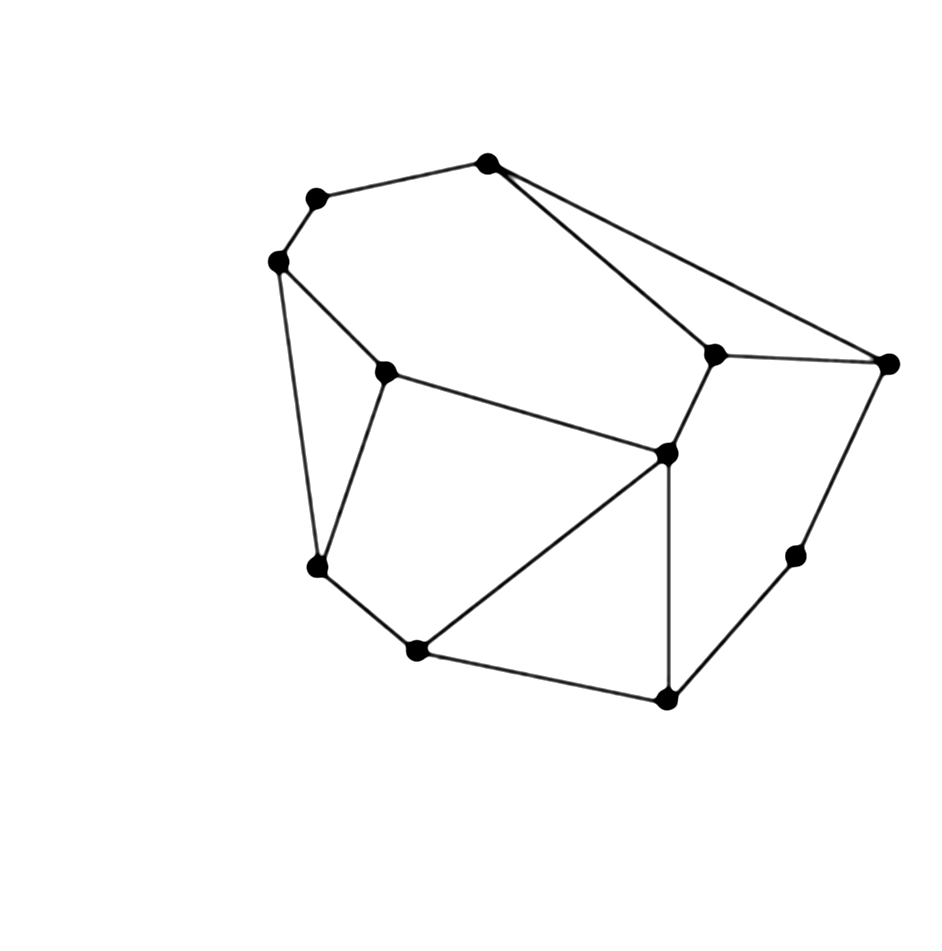
\includegraphics[height=6cm]{figs/pp1} \end{center} We have a set of any possible outcomes \end{figure} \end{frame}
\begin{frame} \frametitle{The GNK value - visual concept} \begin{figure} \begin{center} 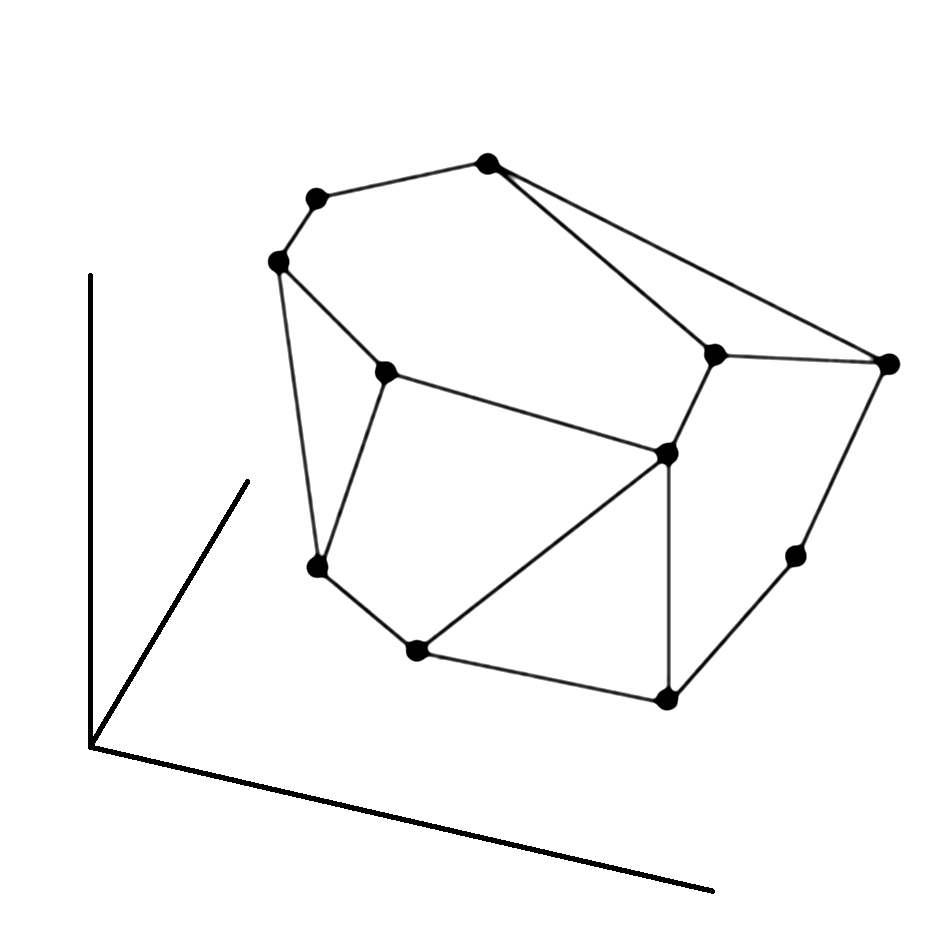
\includegraphics[height=6cm]{figs/pp2} \end{center} Which result from actions \end{figure} \end{frame}
\begin{frame} \frametitle{The GNK value - visual concept} \begin{figure} \begin{center} 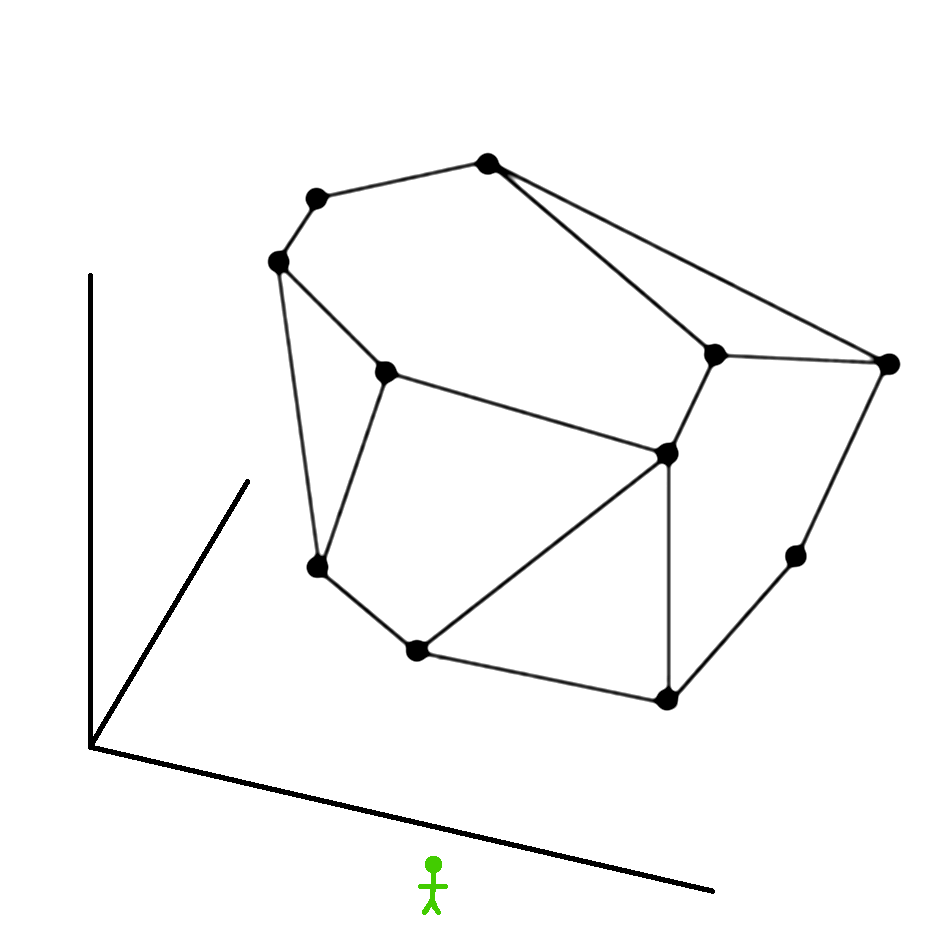
\includegraphics[height=6cm]{figs/pp3} \end{center} the actions of individuals \end{figure} \end{frame}
\begin{frame} \frametitle{The GNK value - visual concept} \begin{figure} \begin{center} 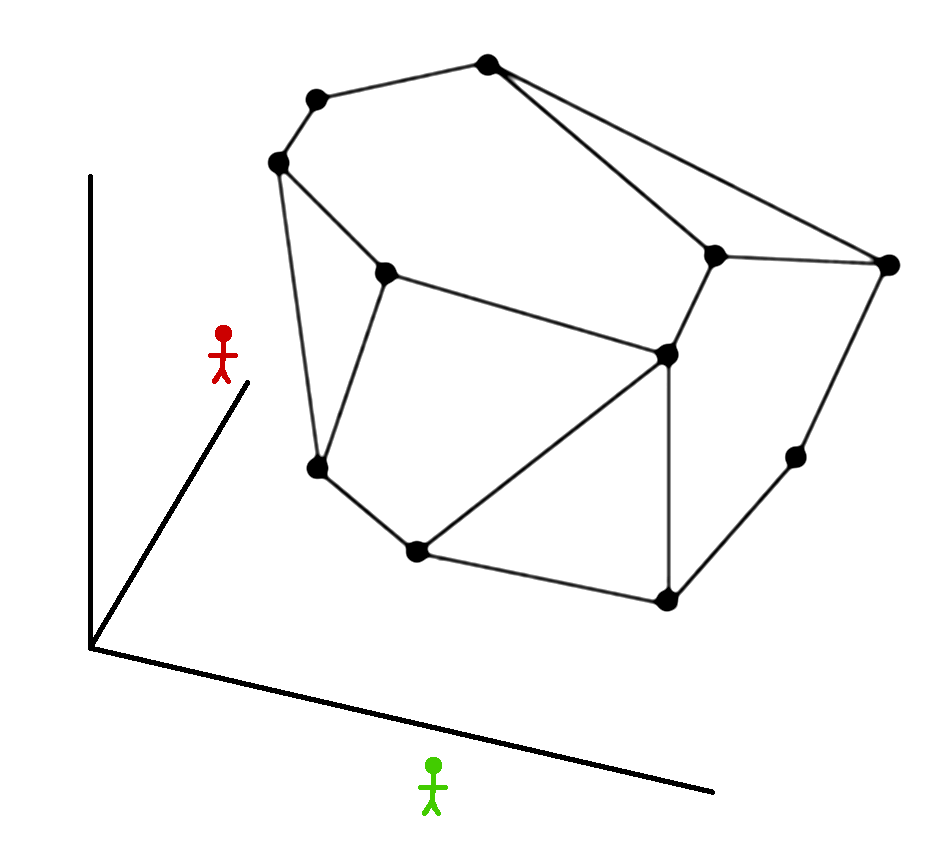
\includegraphics[height=6cm]{figs/pp4} \end{center} the actions of individuals \end{figure} \end{frame}
\begin{frame} \frametitle{The GNK value - visual concept} \begin{figure} \begin{center} 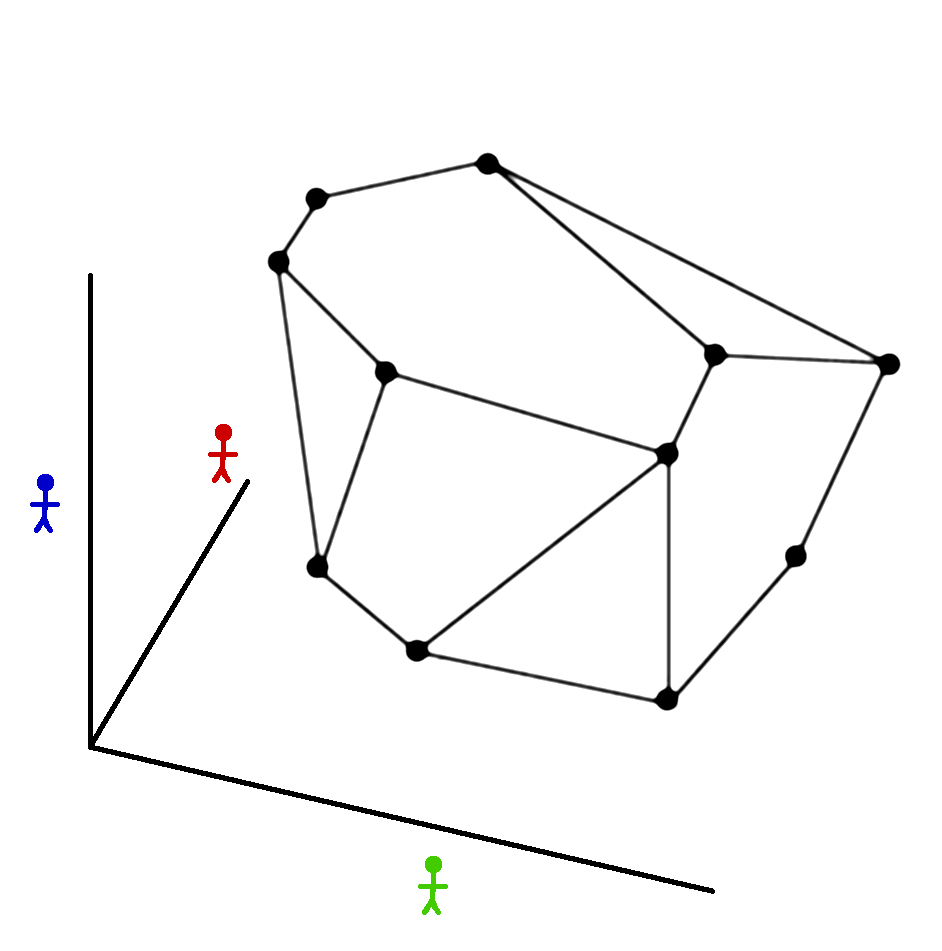
\includegraphics[height=6cm]{figs/pp5} \end{center} the actions of individuals \end{figure} \end{frame}
\begin{frame} \frametitle{The GNK value - visual concept} \begin{figure} \begin{center} 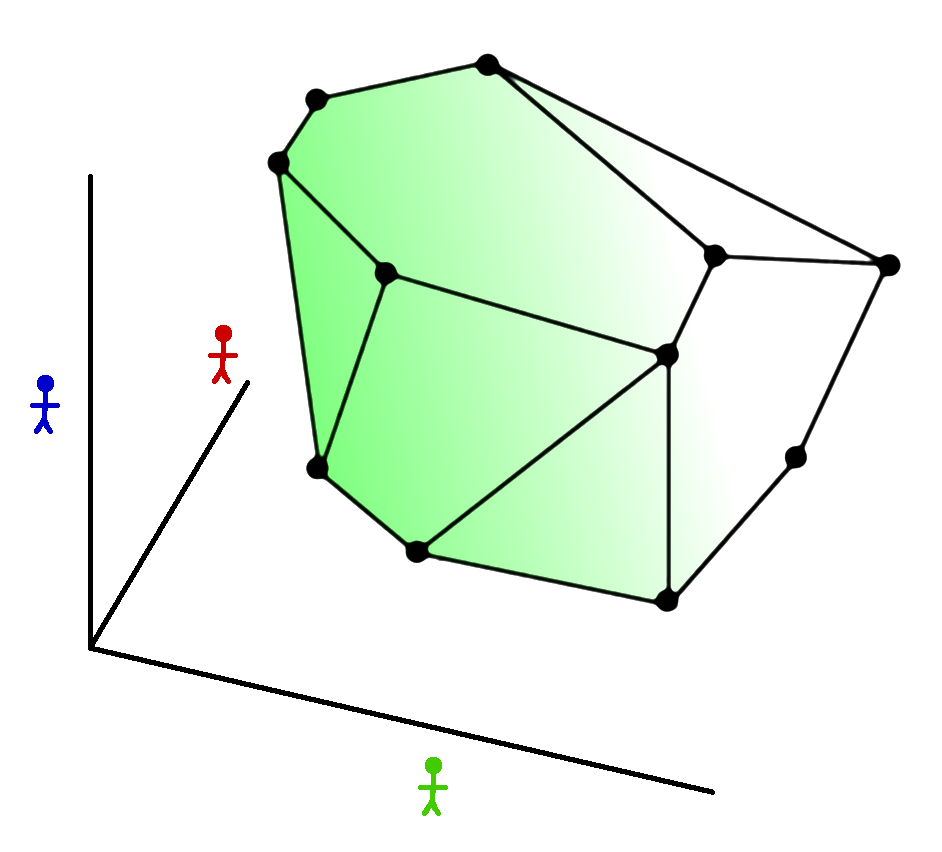
\includegraphics[height=6cm]{figs/pp6} \end{center} individuals value outcomes differently \end{figure} \end{frame}
\begin{frame} \frametitle{The GNK value - visual concept} \begin{figure} \begin{center} 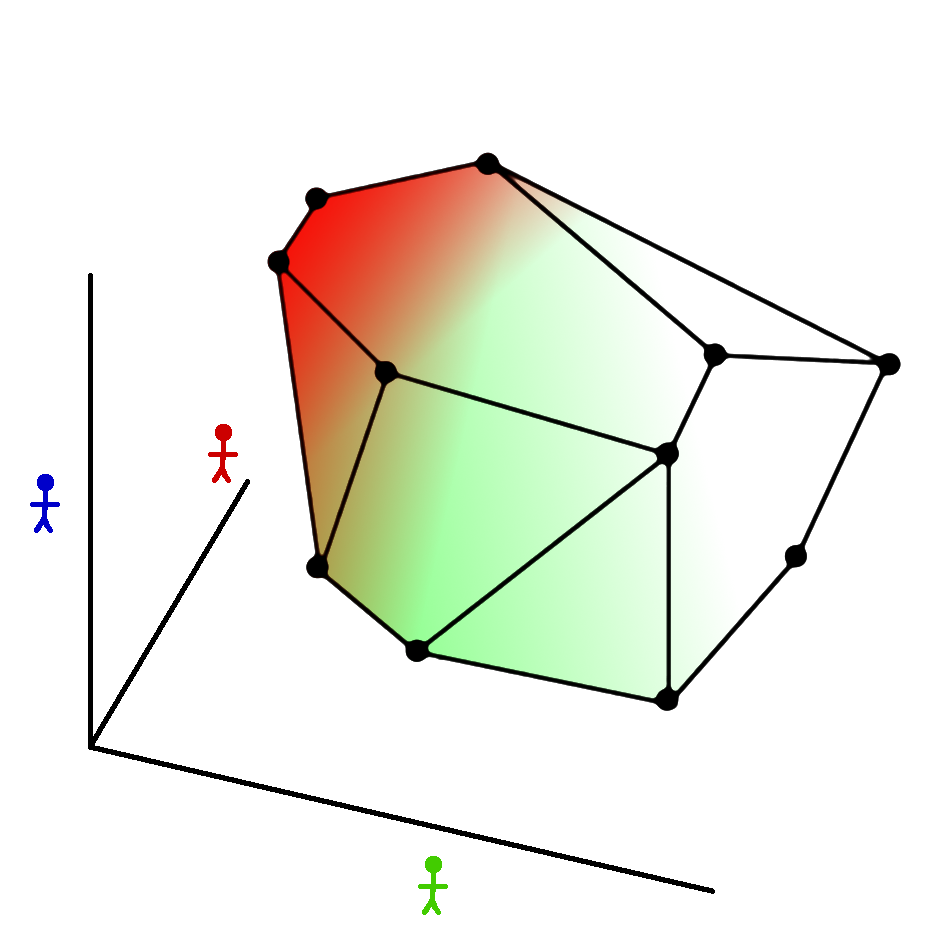
\includegraphics[height=6cm]{figs/pp7} \end{center} individuals value outcomes differently \end{figure} \end{frame}
\begin{frame} \frametitle{The GNK value - visual concept} \begin{figure} \begin{center} 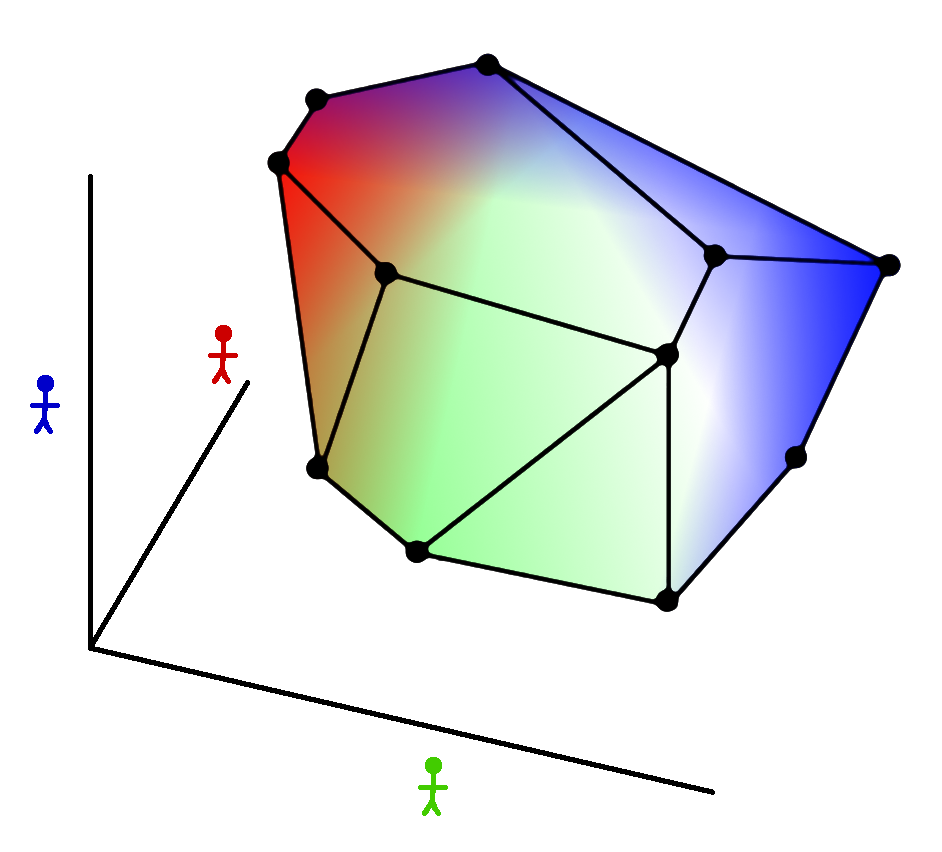
\includegraphics[height=6cm]{figs/pp8} \end{center} individuals value outcomes differently \end{figure} \end{frame}
\begin{frame} \frametitle{The GNK value - visual concept} \begin{figure} \begin{center} 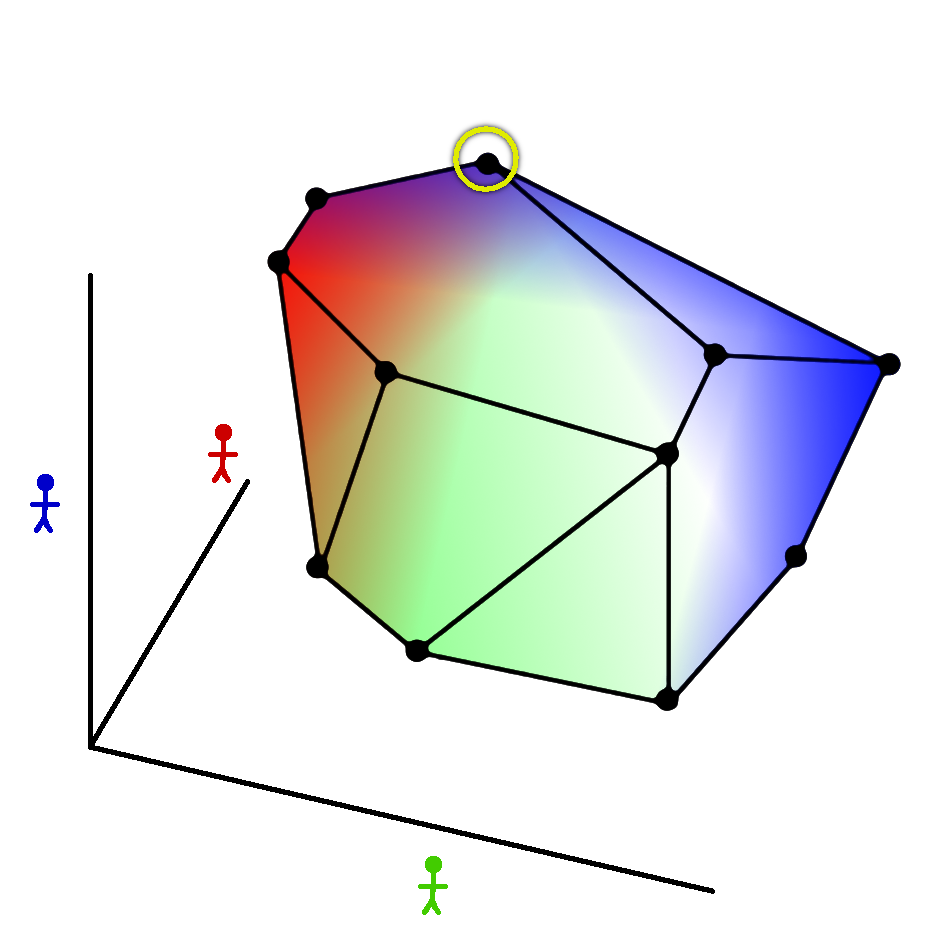
\includegraphics[height=6cm]{figs/pp9} \end{center} yeilding a socially optimal outcome \end{figure} \end{frame}
\begin{frame} \frametitle{The GNK value - visual concept} \begin{figure} \begin{center} 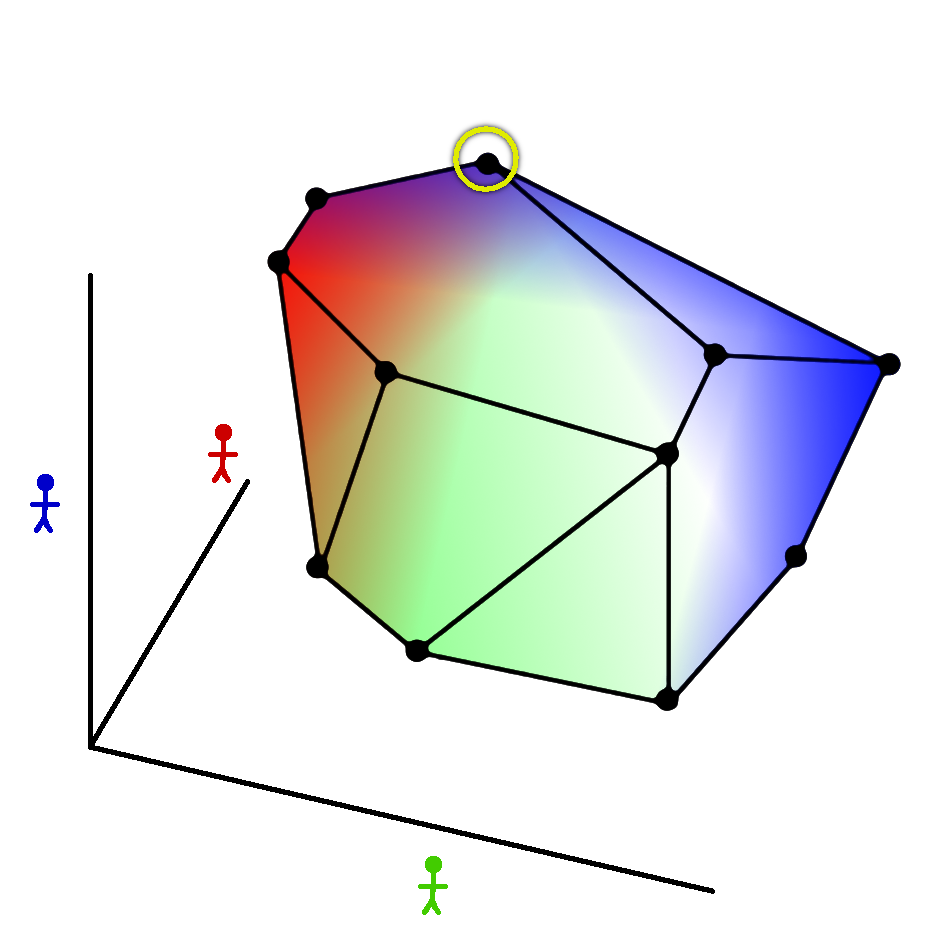
\includegraphics[height=6cm]{figs/pp9} \end{center} yeilding a socially optimal outcome \\ but how much should each pay? \end{figure} \end{frame}



\begin{frame}
\frametitle{The GNK value}
We consider \textit{generalized non-cooperative game} in which:
\begin{itemize}
\item	$N=\{1,\dots,n\}$ is a finite set of players,
\item	$A\subseteq \prod_{i\in N}A^i$ is a set of all possible joint strategies, where $A^i$ denotes the set of strategies available to player $i\in N$.
\item	$\{u_i(a) : A\rightarrow \mathbb{R}\}_{i\in N}$ is a set of functions of each player's payoff/utility when joint strategy $a\in A$ is executed.
\end{itemize}

In this context, we wish to describe the payoff `threat' or `advantage' $v(S)$ of a coalition $S\subseteq N$.
\end{frame}





\begin{frame} \frametitle{The GNK value - visual concept part 2} \begin{figure} \begin{center} 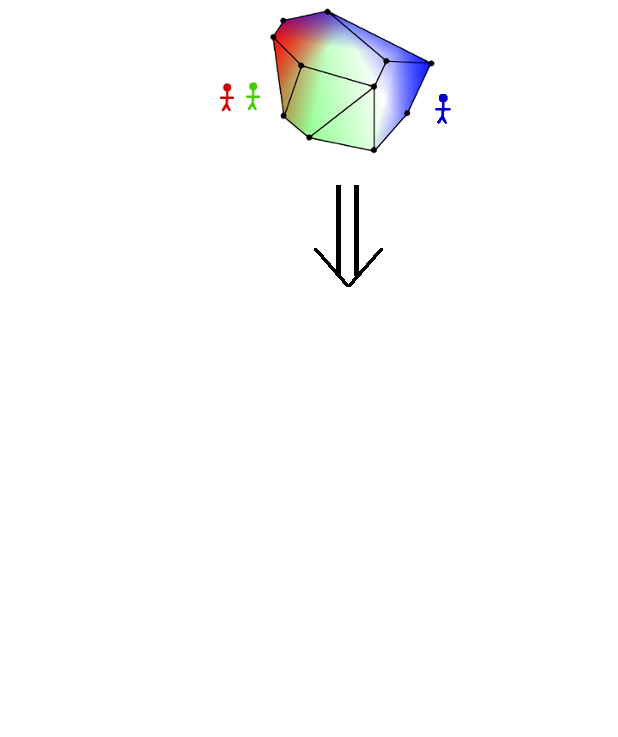
\includegraphics[height=7cm]{figs/pa1} \end{center} We have to break it up \end{figure} \end{frame}
\begin{frame} \frametitle{The GNK value - visual concept part 2} \begin{figure} \begin{center} 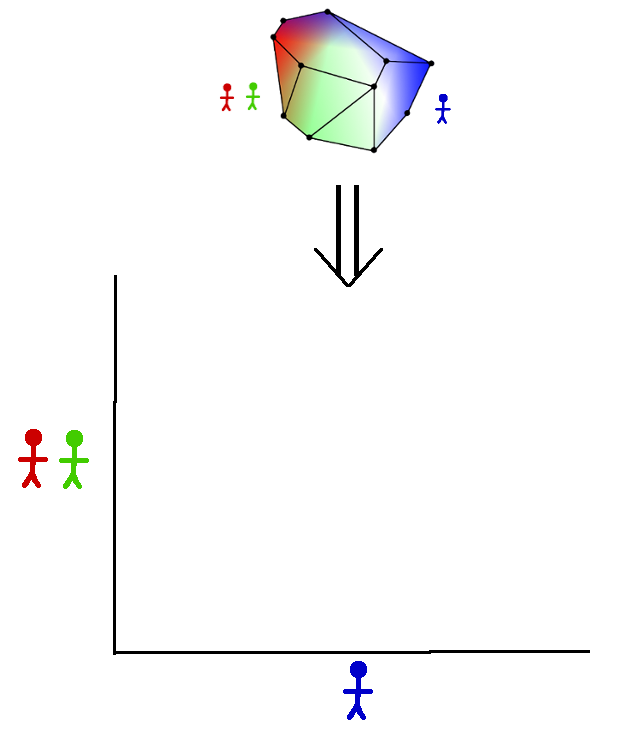
\includegraphics[height=7cm]{figs/pa2} \end{center} Into two coalitions \end{figure} \end{frame}
\begin{frame} \frametitle{The GNK value - visual concept part 2} \begin{figure} \begin{center} 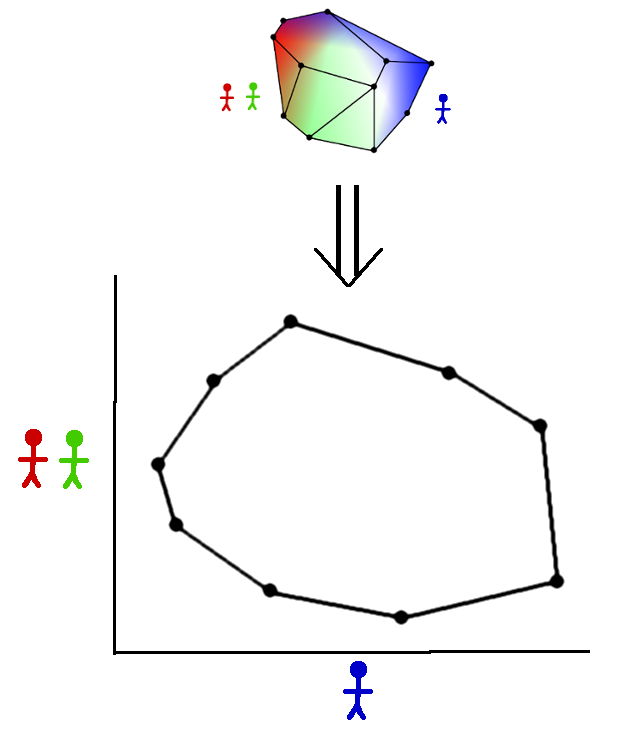
\includegraphics[height=7cm]{figs/pa3} \end{center} the space of outcomes between the coalitions \end{figure} \end{frame}
\begin{frame} \frametitle{The GNK value - visual concept part 2} \begin{figure} \begin{center} 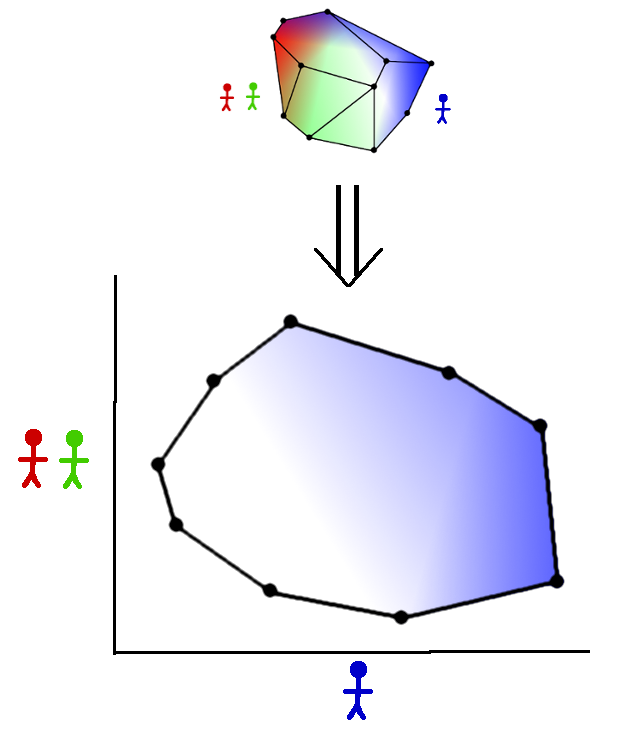
\includegraphics[height=7cm]{figs/pa4} \end{center} ... has value to each coalition \end{figure} \end{frame}
\begin{frame} \frametitle{The GNK value - visual concept part 2} \begin{figure} \begin{center} 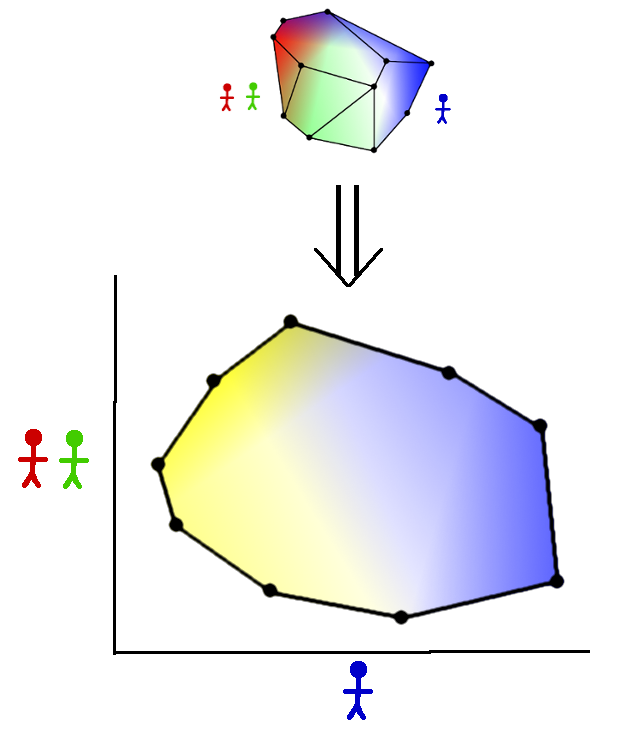
\includegraphics[height=7cm]{figs/pa5} \end{center} ... has value to each coalition \end{figure} \end{frame}
\begin{frame} \frametitle{The GNK value - visual concept part 2} \begin{figure} \begin{center} 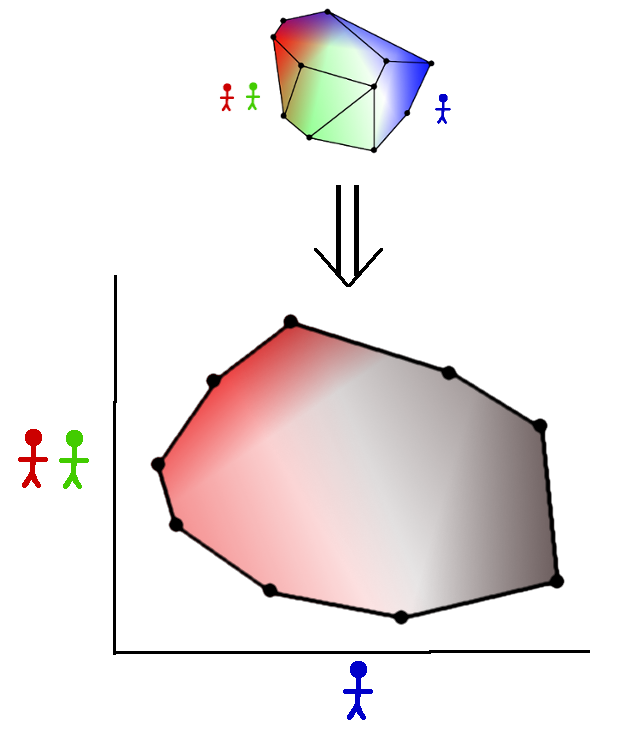
\includegraphics[height=7cm]{figs/pa6} \end{center} We consider the payoff advantage one has over the other \end{figure} \end{frame}
\begin{frame} \frametitle{The GNK value - visual concept part 2} \begin{figure} \begin{center} 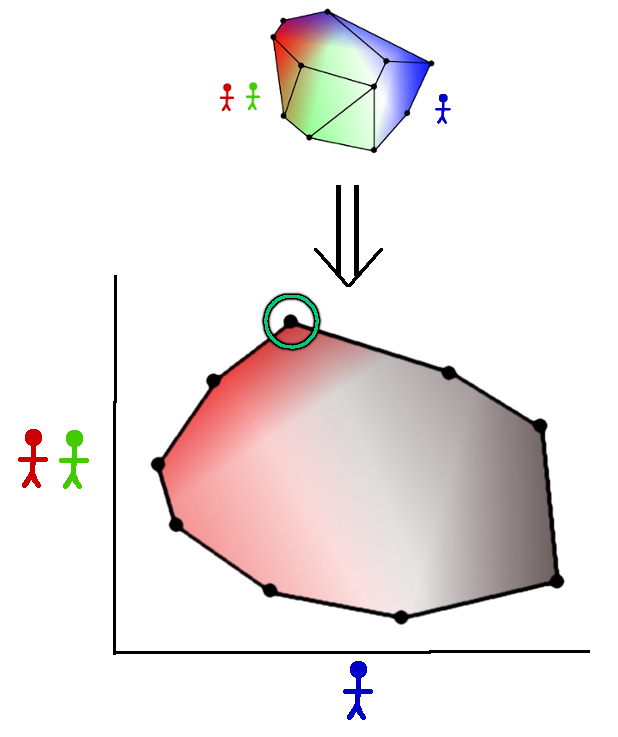
\includegraphics[height=7cm]{figs/pa7} \end{center} what is the guaranteed payoff advantage if one goes first \end{figure} \end{frame}
\begin{frame} \frametitle{The GNK value - visual concept part 2} \begin{figure} \begin{center} 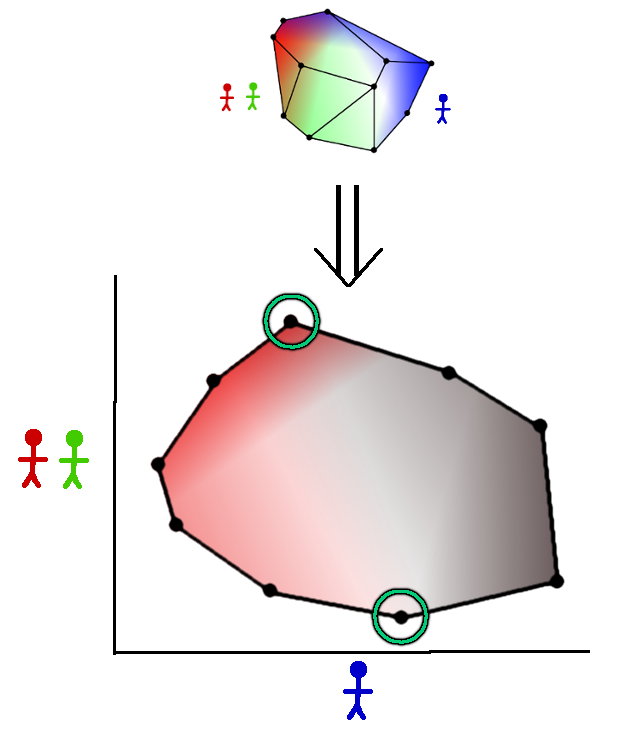
\includegraphics[height=7cm]{figs/pa8} \end{center} what is the guaranteed payoff advantage if the other goes first \end{figure} \end{frame}
\begin{frame} \frametitle{The GNK value - visual concept part 2} \begin{figure} \begin{center} 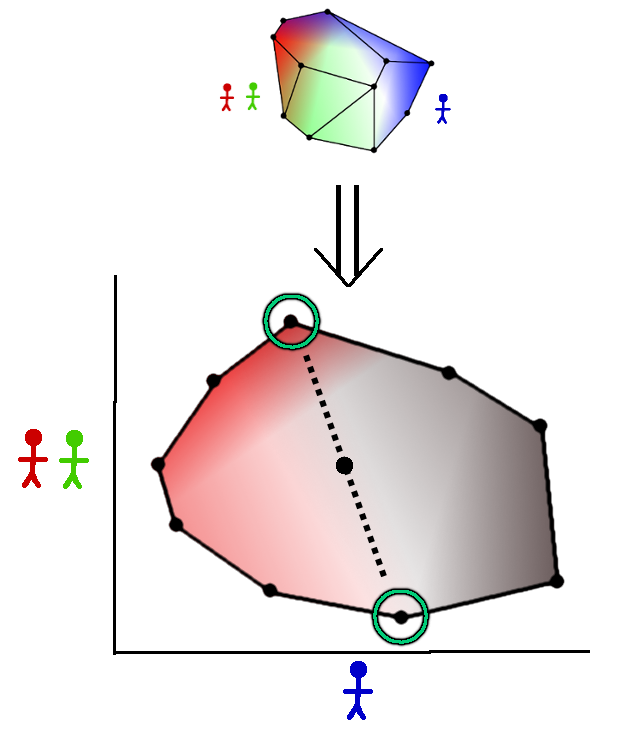
\includegraphics[height=7cm]{figs/pa9} \end{center} average these minimax payoff advantages \end{figure} \end{frame}







\begin{frame}
\frametitle{The GNK value}
Denoting $(x,y)\in A$ as a partition of a joint action between two coalitions $S$ and $N\setminus S$, 
the characteristic function for the game of threats with generalised action spaces is given by:
\begin{align}
\label{knvalue1}
v(S) = &
\frac{1}{2}\min_{\substack{y\in A^{N\setminus S} \\ \text{s.t.}\exists x,(x,y)\in A}} 
\max_{\substack{x\in A^S \\ \text{s.t.}(x,y)\in A}}
	\left(\sum_{i\in S} u_i(x,y) - \sum_{i\in N\setminus S}u_i(x,y)\right)\nonumber\\
+&
\frac{1}{2}\max_{\substack{x\in A^S \\ \text{s.t.}\exists y,(x,y)\in A}}
\min_{\substack{y\in A^{N\setminus S} \\ \text{s.t.}(x,y)\in A}}
	\left(\sum_{i\in S} u_i(x,y) - \sum_{i\in N\setminus S} u_i(x,y) \right)
\end{align}

We wish to aggregate these payoff advantages, or `threat', via axioms.
\end{frame}


\begin{frame}
\frametitle{The GNK value}
It is proven that if $\mathbb{D}$ is the set of all such games, then there exists a unique mapping $\varphi:\mathbb{D}\rightarrow\mathbb{R}^n$ that satisfies Shapley style axioms:

\begin{itemize}
\item	\textbf{Efficiency}: $\sum_i\varphi(\langle N,v\rangle)_i = v(N)\qquad\qquad\qquad\qquad\qquad\qquad\qquad\qquad\qquad~~\refstepcounter{equation}(\theequation)\label{myeq}$
\item	\textbf{Symmetry}: If two players $i$ and $j$ are substitutes, such that if $v(S\cup i)=v(S\cup j)~~\forall S\subseteq N\setminus\{i,j\}$, then $\varphi(\langle N,v\rangle)_i = \varphi(\langle N,v\rangle)_j$
\item	\textbf{Null Player}: If a player $i$ is a null player (i.e.\ $v(S\cup i)=v(S)~~\forall S\subseteq N$) then $\varphi(\langle N,v\rangle)_i=0$
\item	\textbf{Additivity}: for any $v_1$ and $v_2$, $\varphi(\langle N,v_1+v_2\rangle)=\varphi(\langle N,v_1 \rangle) + \varphi(\langle N,v_2\rangle)$
\end{itemize}

Letting agent $i$'s element of $\varphi$ be denoted by $\varphi_i$, this mapping is:
\begin{equation}\label{da_value_eq} 
\varphi_i(\langle N,v\rangle)
= \frac{1}{n}\sum_{k=1}^n v_{i,k} 
= \frac{1}{n}\sum_{k=1}^n \frac{1}{\binom{n-1}{k-1}} \sum_{\substack{S:i\in S \\ |S|=k}}v(S) 
\end{equation}
\end{frame}



\begin{frame}
\frametitle{Okay... that is nice}
Why do it this way?

Links directly to well established literature on bargaining:
\begin{itemize}
\item	John Nash
\item	John Harsanyi
\item	Kalai \& Kalai
\item	Neyman \& Kohlberg
\end{itemize}
Directly adjacent to other historic formulations
\begin{itemize}
\item	Aumann $\alpha$ and $\beta$ solution concepts
\item	von Neumann \& Mortgenstein solution
\end{itemize}

Historic Game-Theory pioneers discussing how to superimpose the Shapley Value over non-cooperative games 
\end{frame}



\begin{frame}
\frametitle{Okay... that is nice}
Why do it this way?

\begin{itemize}
\item	Considers whole strategy space
\item	model of perfect competition of divergent interests and leverage between all parties
\item	it is efficient
\item	it is budget balanced
\item	Shapley Value axiomatic
\end{itemize}
\end{frame}


\begin{frame}
\frametitle{The GNK value}
Indeed \cite{KOHLBERG2018139} have shown that for any game of threats $\langle N,v\rangle$ there is a classic cooperative game $\langle N,v'\rangle$ where the two Shapley values are the same.
It is possible to map a game of threats $v$ to a cooperative game $v'$ via relation:
\begin{equation}\label{convert1}
v'(S)=\frac{1}{2}v(S)+\frac{1}{2}v(N)
\end{equation}
\end{frame}



\section{Application}

\begin{frame}
\frametitle{Application to Electricity network}
We consider an electricity network under DC approximation:
\begin{itemize}
    \item A set of buses $B$ with, for all $i\in B$:
    \begin{itemize} 
        \item Power consumption at each bus $p_i$, and 
        \item A bus voltage phase-angle $\theta_i$,
    \end{itemize}
    \item Lines $C\subseteq B\times B$, with, for all $(i,j)\in C$: 
        \begin{itemize} 
        \item Line susceptance $b_{i,j}$, and 
        \item Power flow $p_{i,j}$ (power from bus $i$ to $j$), with $p_{i,j}=-p_{j,i}$. 
    \end{itemize}
\end{itemize}

One player per bus (i.e.~$N=B$), and the power consumption of that bus is the player's strategy space (i.e.\ $A_i=[p_i^l,p_i^u]$).
And a linear utility associated with the power consumption of each player, $u_i(p_i)$
\end{frame}

\begin{frame}
\begin{figure}[]
\includegraphics[width=0.45\linewidth,height=0.4\linewidth]{figs/GNK5.tikz}%
\resizebox*{0.35\linewidth} {!} {
    \begin {tikzpicture}
		\draw[line width=3pt] (0,0) -- (4,0);
		\draw[line width=3pt] (-2,-3) -- (2,-3);
		\draw[-{Latex[length=5mm, width=4mm]},line width=3pt] (-1,-3) -- (-1,-4);
		\draw[line width=3pt] (1,-4) -- (5,-4);
		\draw[-{Latex[length=5mm, width=4mm]},line width=3pt] (2,-4) -- (2,-5);
		\draw[line width=3pt] (4,-5) -- (8,-5);
		\draw[-{Latex[length=5mm, width=4mm]},line width=3pt] (5,-5) -- (5,-6);
		\draw[line width=3pt] (2,-7) -- (6,-7);
		\draw[-{Latex[length=5mm, width=4mm]},line width=3pt] (3,-7) -- (3,-8);

		\draw[line width=1pt] (1,0) -- (1,-1);
		\draw[line width=1pt] (1,-1) -- (0,-2);
		\draw[line width=1pt] (0,-2) -- (0,-3);

		\draw[line width=1pt] (2,0) -- (2,-1);
		\draw[line width=1pt] (2,-1) -- (3,-2);
		\draw[line width=1pt] (3,-2) -- (3,-4);

		\draw[line width=1pt] (3,0) -- (3,-1);
		\draw[line width=1pt] (3,-1) -- (6,-2);
		\draw[line width=1pt] (6,-2) -- (6,-5);
		
		
		\draw[line width=1pt] (3.5,-4) -- (3.5,-7);

		\draw[line width=1pt] (2.2,0) -- (2.2,1);
		\draw (2.2,1.5) circle (0.5);
		\draw (1.9,1.5) .. controls (1.9+0.2,1.5+0.7) and (2.5-0.2,1.5-0.7) .. (2.5,1.5);

		\node (text) at (4.1,0+0.4) {\scalebox{1.9}{1}};
		\node (text) at (2.1,-3+0.4) {\scalebox{1.9}{2}};
		\node (text) at (5.1,-4+0.4) {\scalebox{1.9}{3}};
		\node (text) at (8.1,-5+0.4) {\scalebox{1.9}{4}};
		\node (text) at (6.1,-7+0.4) {\scalebox{1.9}{5}};
    \end {tikzpicture}
}
\end{figure}
LMP transfers for Example network
\end{frame}


\begin{frame}
\begin{figure}[]
\includegraphics[width=0.45\linewidth,height=0.4\linewidth]{figs/GNK8.tikz}%
\resizebox*{0.35\linewidth} {!} {
    \begin {tikzpicture}
		\draw[line width=3pt] (0,0) -- (4,0);
		\draw[line width=3pt] (-2,-3) -- (2,-3);
		\draw[-{Latex[length=5mm, width=4mm]},line width=3pt] (-1,-3) -- (-1,-4);
		\draw[line width=3pt] (1,-4) -- (5,-4);
		\draw[-{Latex[length=5mm, width=4mm]},line width=3pt] (2,-4) -- (2,-5);
		\draw[line width=3pt] (4,-5) -- (8,-5);
		\draw[-{Latex[length=5mm, width=4mm]},line width=3pt] (5,-5) -- (5,-6);
		\draw[line width=3pt] (2,-7) -- (6,-7);
		\draw[-{Latex[length=5mm, width=4mm]},line width=3pt] (3,-7) -- (3,-8);

		\draw[line width=1pt] (1,0) -- (1,-1);
		\draw[line width=1pt] (1,-1) -- (0,-2);
		\draw[line width=1pt] (0,-2) -- (0,-3);

		\draw[line width=1pt] (2,0) -- (2,-1);
		\draw[line width=1pt] (2,-1) -- (3,-2);
		\draw[line width=1pt] (3,-2) -- (3,-4);

		\draw[line width=1pt] (3,0) -- (3,-1);
		\draw[line width=1pt] (3,-1) -- (6,-2);
		\draw[line width=1pt] (6,-2) -- (6,-5);
		
		
		\draw[line width=1pt] (3.5,-4) -- (3.5,-7);

		\draw[line width=1pt] (2.2,0) -- (2.2,1);
		\draw (2.2,1.5) circle (0.5);
		\draw (1.9,1.5) .. controls (1.9+0.2,1.5+0.7) and (2.5-0.2,1.5-0.7) .. (2.5,1.5);

		\node (text) at (4.1,0+0.4) {\scalebox{1.9}{1}};
		\node (text) at (2.1,-3+0.4) {\scalebox{1.9}{2}};
		\node (text) at (5.1,-4+0.4) {\scalebox{1.9}{3}};
		\node (text) at (8.1,-5+0.4) {\scalebox{1.9}{4}};
		\node (text) at (6.1,-7+0.4) {\scalebox{1.9}{5}};
    \end {tikzpicture}
}
\end{figure}
VCG transfers for Example network
\end{frame}


\begin{frame}
\begin{figure}[]
\includegraphics[width=0.45\linewidth,height=0.4\linewidth]{figs/GNK4.tikz}%
\resizebox*{0.35\linewidth} {!} {
    \begin {tikzpicture}
		\draw[line width=3pt] (0,0) -- (4,0);
		\draw[line width=3pt] (-2,-3) -- (2,-3);
		\draw[-{Latex[length=5mm, width=4mm]},line width=3pt] (-1,-3) -- (-1,-4);
		\draw[line width=3pt] (1,-4) -- (5,-4);
		\draw[-{Latex[length=5mm, width=4mm]},line width=3pt] (2,-4) -- (2,-5);
		\draw[line width=3pt] (4,-5) -- (8,-5);
		\draw[-{Latex[length=5mm, width=4mm]},line width=3pt] (5,-5) -- (5,-6);
		\draw[line width=3pt] (2,-7) -- (6,-7);
		\draw[-{Latex[length=5mm, width=4mm]},line width=3pt] (3,-7) -- (3,-8);

		\draw[line width=1pt] (1,0) -- (1,-1);
		\draw[line width=1pt] (1,-1) -- (0,-2);
		\draw[line width=1pt] (0,-2) -- (0,-3);

		\draw[line width=1pt] (2,0) -- (2,-1);
		\draw[line width=1pt] (2,-1) -- (3,-2);
		\draw[line width=1pt] (3,-2) -- (3,-4);

		\draw[line width=1pt] (3,0) -- (3,-1);
		\draw[line width=1pt] (3,-1) -- (6,-2);
		\draw[line width=1pt] (6,-2) -- (6,-5);
		
		
		\draw[line width=1pt] (3.5,-4) -- (3.5,-7);

		\draw[line width=1pt] (2.2,0) -- (2.2,1);
		\draw (2.2,1.5) circle (0.5);
		\draw (1.9,1.5) .. controls (1.9+0.2,1.5+0.7) and (2.5-0.2,1.5-0.7) .. (2.5,1.5);

		\node (text) at (4.1,0+0.4) {\scalebox{1.9}{1}};
		\node (text) at (2.1,-3+0.4) {\scalebox{1.9}{2}};
		\node (text) at (5.1,-4+0.4) {\scalebox{1.9}{3}};
		\node (text) at (8.1,-5+0.4) {\scalebox{1.9}{4}};
		\node (text) at (6.1,-7+0.4) {\scalebox{1.9}{5}};
    \end {tikzpicture}
}
\end{figure}
GNK transfers for example network
\end{frame}

\begin{frame}
\frametitle{Qualities of GNK}
\begin{itemize}
\item	The GNK value is continuous in the parameters of the network
\item	The GNK payments are always budget balanced
\item	The GNK value can offset those that do not receive or generate power
\item	The GNK value is not incentive compatible
\item	The GNK value is computationally difficult
\end{itemize}
Is the GNK value the right way?
\end{frame}

\section{Extending to larger networks}

\begin{frame}
\frametitle{Scaling to larger Networks}
Approaches:
\begin{itemize}
\item	Sampling techniques
\item	Simplifying Proxy for minimax optimisations
\end{itemize}
\end{frame}

\begin{frame}
\frametitle{Sampling}
To sample the GNK value either A) directly or B) by converting it to Shapley Value.
if B) is sampling is conducted in a join ordering, and using stratification?.
particularly stratification is used whether equation \ref{shapley_value1} is used over or \ref{shapley_value3} more directly.
A range of sampling methods:

\begin{itemize}
\item	\textsc{Simple}: For sampling the GNK value directly per equation \ref{da_value_eq}, stratification approximating each $v_{i,k}$ 
\item	\textsc{Appro}: For sampling the Shapley Value directly without stratification by sampling equation \ref{shapley_value3}. \cite{DBLP:journals/cor/CastroGT09}
\item	\textsc{Join}: For sampling the Shapley Value using stratification equation \ref{shapley_value1} using join orders. \cite{CASTRO2017180}
\item	\textsc{Neyman}: For sampling the Shapley Value using stratification equation \ref{shapley_value1}, not using join orders, in proportion to the sample variance of the strata, expending half the budget attaining variances before sampling in proportion to them. \cite{CASTRO2017180,1938.10503378}
\item	\textsc{Hoeffding}: For sampling the Shapley Value using stratification equation \ref{shapley_value1}, not using join orders, in proportion to a Hoeffding type inequality on the error of the strata estimates \cite{2013arXiv1306.4265M}
\item	\textsc{SEBM}: For sampling the Shapley Value using stratification, not using join orders, in association with a complicated concentration inequality developed by us.
\end{itemize}
\end{frame}

\begin{frame}

    \begin{figure}[]
        \centering
		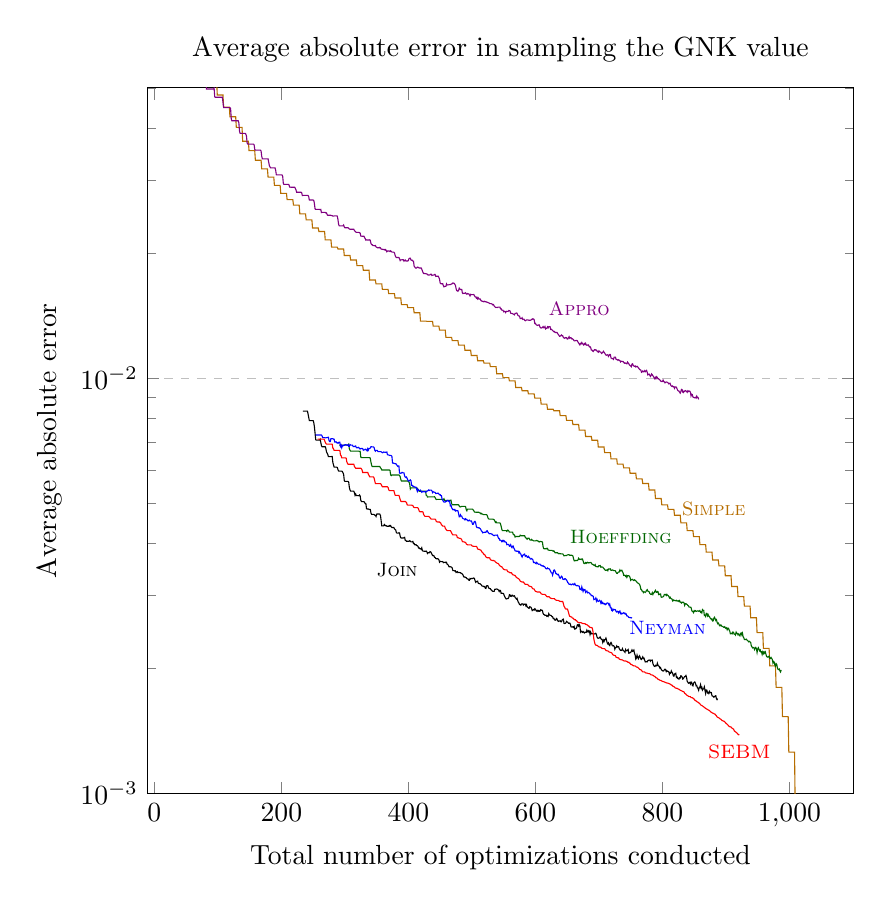
\begin{tikzpicture}
		\begin{axis}[
			title={Average absolute error in sampling the GNK value},
			xlabel={Total number of optimizations conducted},
			ylabel={Average absolute error},
			%xmin=0, xmax=0.25,
			ymin=0.001, ymax=0.05,
			ymode=log,
			%xtick={0,0.05,0.1,0.15,0.2,0.25},
			%ytick={0,20,40,60,80,100},
			%yticklabel=$\pgfmathprintnumber{\tick}\%$,
			legend pos=south west,
			ymajorgrids=true,
			grid style=dashed,
			%xticklabel style={/pgf/number format/fixed}
			width = 300,
			height = 300
		]
		\addplot[color={rgb:red,4;green,2;yellow,1}] coordinates {
(39,0.0905511314206)(40,0.0905511314206)(41,0.0905511314206)(42,0.0905511314206)(43,0.0905511314206)(44,0.0905511314206)(45,0.0905511314206)(46,0.0905511314206)(47,0.0905511314206)(48,0.0905511314206)(49,0.0800346783099)(50,0.0800346783099)(51,0.0800346783099)(52,0.0800346783099)(53,0.0800346783099)(54,0.0800346783099)(55,0.0800346783099)(56,0.0800346783099)(57,0.0800346783099)(58,0.0800346783099)(59,0.0726818288329)(60,0.0726818288329)(61,0.0726818288329)(62,0.0726818288329)(63,0.0726818288329)(64,0.0726818288329)(65,0.0726818288329)(66,0.0726818288329)(67,0.0726818288329)(68,0.0726818288329)(69,0.0639984808006)(70,0.0639984808006)(71,0.0639984808006)(72,0.0639984808006)(73,0.0639984808006)(74,0.0639984808006)(75,0.0639984808006)(76,0.0639984808006)(77,0.0639984808006)(78,0.0639984808006)(79,0.0589371626675)(80,0.0589371626675)(81,0.0589371626675)(82,0.0589371626675)(83,0.0589371626675)(84,0.0589371626675)(85,0.0589371626675)(86,0.0589371626675)(87,0.0589371626675)(88,0.0589371626675)(89,0.0520142601085)(90,0.0520142601085)(91,0.0520142601085)(92,0.0520142601085)(93,0.0520142601085)(94,0.0520142601085)(95,0.0520142601085)(96,0.0520142601085)(97,0.0520142601085)(98,0.0520142601085)(99,0.0480768858393)(100,0.0480768858393)(101,0.0480768858393)(102,0.0480768858393)(103,0.0480768858393)(104,0.0480768858393)(105,0.0480768858393)(106,0.0480768858393)(107,0.0480768858393)(108,0.0480768858393)(109,0.0449401631859)(110,0.0449401631859)(111,0.0449401631859)(112,0.0449401631859)(113,0.0449401631859)(114,0.0449401631859)(115,0.0449401631859)(116,0.0449401631859)(117,0.0449401631859)(118,0.0449401631859)(119,0.0426158587744)(120,0.0426158587744)(121,0.0426158587744)(122,0.0426158587744)(123,0.0426158587744)(124,0.0426158587744)(125,0.0426158587744)(126,0.0426158587744)(127,0.0426158587744)(128,0.0426158587744)(129,0.0401740115504)(130,0.0401740115504)(131,0.0401740115504)(132,0.0401740115504)(133,0.0401740115504)(134,0.0401740115504)(135,0.0401740115504)(136,0.0401740115504)(137,0.0401740115504)(138,0.0401740115504)(139,0.0372039977439)(140,0.0372039977439)(141,0.0372039977439)(142,0.0372039977439)(143,0.0372039977439)(144,0.0372039977439)(145,0.0372039977439)(146,0.0372039977439)(147,0.0372039977439)(148,0.0372039977439)(149,0.0353250731826)(150,0.0353250731826)(151,0.0353250731826)(152,0.0353250731826)(153,0.0353250731826)(154,0.0353250731826)(155,0.0353250731826)(156,0.0353250731826)(157,0.0353250731826)(158,0.0353250731826)(159,0.0334827529779)(160,0.0334827529779)(161,0.0334827529779)(162,0.0334827529779)(163,0.0334827529779)(164,0.0334827529779)(165,0.0334827529779)(166,0.0334827529779)(167,0.0334827529779)(168,0.0334827529779)(169,0.0319278878629)(170,0.0319278878629)(171,0.0319278878629)(172,0.0319278878629)(173,0.0319278878629)(174,0.0319278878629)(175,0.0319278878629)(176,0.0319278878629)(177,0.0319278878629)(178,0.0319278878629)(179,0.0304839904472)(180,0.0304839904472)(181,0.0304839904472)(182,0.0304839904472)(183,0.0304839904472)(184,0.0304839904472)(185,0.0304839904472)(186,0.0304839904472)(187,0.0304839904472)(188,0.0304839904472)(189,0.0291191466057)(190,0.0291191466057)(191,0.0291191466057)(192,0.0291191466057)(193,0.0291191466057)(194,0.0291191466057)(195,0.0291191466057)(196,0.0291191466057)(197,0.0291191466057)(198,0.0291191466057)(199,0.0278671669628)(200,0.0278671669628)(201,0.0278671669628)(202,0.0278671669628)(203,0.0278671669628)(204,0.0278671669628)(205,0.0278671669628)(206,0.0278671669628)(207,0.0278671669628)(208,0.0278671669628)(209,0.0269069097188)(210,0.0269069097188)(211,0.0269069097188)(212,0.0269069097188)(213,0.0269069097188)(214,0.0269069097188)(215,0.0269069097188)(216,0.0269069097188)(217,0.0269069097188)(218,0.0269069097188)(219,0.0260967155637)(220,0.0260967155637)(221,0.0260967155637)(222,0.0260967155637)(223,0.0260967155637)(224,0.0260967155637)(225,0.0260967155637)(226,0.0260967155637)(227,0.0260967155637)(228,0.0260967155637)(229,0.0248749696626)(230,0.0248749696626)(231,0.0248749696626)(232,0.0248749696626)(233,0.0248749696626)(234,0.0248749696626)(235,0.0248749696626)(236,0.0248749696626)(237,0.0248749696626)(238,0.0248749696626)(239,0.0240630795676)(240,0.0240630795676)(241,0.0240630795676)(242,0.0240630795676)(243,0.0240630795676)(244,0.0240630795676)(245,0.0240630795676)(246,0.0240630795676)(247,0.0240630795676)(248,0.0240630795676)(249,0.0229955441136)(250,0.0229955441136)(251,0.0229955441136)(252,0.0229955441136)(253,0.0229955441136)(254,0.0229955441136)(255,0.0229955441136)(256,0.0229955441136)(257,0.0229955441136)(258,0.0229955441136)(259,0.022549785203)(260,0.022549785203)(261,0.022549785203)(262,0.022549785203)(263,0.022549785203)(264,0.022549785203)(265,0.022549785203)(266,0.022549785203)(267,0.022549785203)(268,0.022549785203)(269,0.0215391100838)(270,0.0215391100838)(271,0.0215391100838)(272,0.0215391100838)(273,0.0215391100838)(274,0.0215391100838)(275,0.0215391100838)(276,0.0215391100838)(277,0.0215391100838)(278,0.0215391100838)(279,0.0206817363819)(280,0.0206817363819)(281,0.0206817363819)(282,0.0206817363819)(283,0.0206817363819)(284,0.0206817363819)(285,0.0206817363819)(286,0.0206817363819)(287,0.0206817363819)(288,0.0206817363819)(289,0.0204659089804)(290,0.0204659089804)(291,0.0204659089804)(292,0.0204659089804)(293,0.0204659089804)(294,0.0204659089804)(295,0.0204659089804)(296,0.0204659089804)(297,0.0204659089804)(298,0.0204659089804)(299,0.0197474301251)(300,0.0197474301251)(301,0.0197474301251)(302,0.0197474301251)(303,0.0197474301251)(304,0.0197474301251)(305,0.0197474301251)(306,0.0197474301251)(307,0.0197474301251)(308,0.0197474301251)(309,0.0192638138498)(310,0.0192638138498)(311,0.0192638138498)(312,0.0192638138498)(313,0.0192638138498)(314,0.0192638138498)(315,0.0192638138498)(316,0.0192638138498)(317,0.0192638138498)(318,0.0192638138498)(319,0.0186633366799)(320,0.0186633366799)(321,0.0186633366799)(322,0.0186633366799)(323,0.0186633366799)(324,0.0186633366799)(325,0.0186633366799)(326,0.0186633366799)(327,0.0186633366799)(328,0.0186633366799)(329,0.0182006027658)(330,0.0182006027658)(331,0.0182006027658)(332,0.0182006027658)(333,0.0182006027658)(334,0.0182006027658)(335,0.0182006027658)(336,0.0182006027658)(337,0.0182006027658)(338,0.0182006027658)(339,0.0172341200202)(340,0.0172341200202)(341,0.0172341200202)(342,0.0172341200202)(343,0.0172341200202)(344,0.0172341200202)(345,0.0172341200202)(346,0.0172341200202)(347,0.0172341200202)(348,0.0172341200202)(349,0.0168660464006)(350,0.0168660464006)(351,0.0168660464006)(352,0.0168660464006)(353,0.0168660464006)(354,0.0168660464006)(355,0.0168660464006)(356,0.0168660464006)(357,0.0168660464006)(358,0.0168660464006)(359,0.0163614719212)(360,0.0163614719212)(361,0.0163614719212)(362,0.0163614719212)(363,0.0163614719212)(364,0.0163614719212)(365,0.0163614719212)(366,0.0163614719212)(367,0.0163614719212)(368,0.0163614719212)(369,0.0159787483327)(370,0.0159787483327)(371,0.0159787483327)(372,0.0159787483327)(373,0.0159787483327)(374,0.0159787483327)(375,0.0159787483327)(376,0.0159787483327)(377,0.0159787483327)(378,0.0159787483327)(379,0.0155992845832)(380,0.0155992845832)(381,0.0155992845832)(382,0.0155992845832)(383,0.0155992845832)(384,0.0155992845832)(385,0.0155992845832)(386,0.0155992845832)(387,0.0155992845832)(388,0.0155992845832)(389,0.0150360607517)(390,0.0150360607517)(391,0.0150360607517)(392,0.0150360607517)(393,0.0150360607517)(394,0.0150360607517)(395,0.0150360607517)(396,0.0150360607517)(397,0.0150360607517)(398,0.0150360607517)(399,0.014787112882)(400,0.014787112882)(401,0.014787112882)(402,0.014787112882)(403,0.014787112882)(404,0.014787112882)(405,0.014787112882)(406,0.014787112882)(407,0.014787112882)(408,0.014787112882)(409,0.0143791385602)(410,0.0143791385602)(411,0.0143791385602)(412,0.0143791385602)(413,0.0143791385602)(414,0.0143791385602)(415,0.0143791385602)(416,0.0143791385602)(417,0.0143791385602)(418,0.0143791385602)(419,0.0137237284373)(420,0.0137237284373)(421,0.0137237284373)(422,0.0137237284373)(423,0.0137237284373)(424,0.0137237284373)(425,0.0137237284373)(426,0.0137237284373)(427,0.0137237284373)(428,0.0137237284373)(429,0.01370085711)(430,0.01370085711)(431,0.01370085711)(432,0.01370085711)(433,0.01370085711)(434,0.01370085711)(435,0.01370085711)(436,0.01370085711)(437,0.01370085711)(438,0.01370085711)(439,0.0133516232869)(440,0.0133516232869)(441,0.0133516232869)(442,0.0133516232869)(443,0.0133516232869)(444,0.0133516232869)(445,0.0133516232869)(446,0.0133516232869)(447,0.0133516232869)(448,0.0133516232869)(449,0.0130557105539)(450,0.0130557105539)(451,0.0130557105539)(452,0.0130557105539)(453,0.0130557105539)(454,0.0130557105539)(455,0.0130557105539)(456,0.0130557105539)(457,0.0130557105539)(458,0.0130557105539)(459,0.0125405867102)(460,0.0125405867102)(461,0.0125405867102)(462,0.0125405867102)(463,0.0125405867102)(464,0.0125405867102)(465,0.0125405867102)(466,0.0125405867102)(467,0.0125405867102)(468,0.0125405867102)(469,0.0123170987621)(470,0.0123170987621)(471,0.0123170987621)(472,0.0123170987621)(473,0.0123170987621)(474,0.0123170987621)(475,0.0123170987621)(476,0.0123170987621)(477,0.0123170987621)(478,0.0123170987621)(479,0.0120153615181)(480,0.0120153615181)(481,0.0120153615181)(482,0.0120153615181)(483,0.0120153615181)(484,0.0120153615181)(485,0.0120153615181)(486,0.0120153615181)(487,0.0120153615181)(488,0.0120153615181)(489,0.0116747189614)(490,0.0116747189614)(491,0.0116747189614)(492,0.0116747189614)(493,0.0116747189614)(494,0.0116747189614)(495,0.0116747189614)(496,0.0116747189614)(497,0.0116747189614)(498,0.0116747189614)(499,0.0113416414427)(500,0.0113416414427)(501,0.0113416414427)(502,0.0113416414427)(503,0.0113416414427)(504,0.0113416414427)(505,0.0113416414427)(506,0.0113416414427)(507,0.0113416414427)(508,0.0113416414427)(509,0.0110141470141)(510,0.0110141470141)(511,0.0110141470141)(512,0.0110141470141)(513,0.0110141470141)(514,0.0110141470141)(515,0.0110141470141)(516,0.0110141470141)(517,0.0110141470141)(518,0.0110141470141)(519,0.0108760396439)(520,0.0108760396439)(521,0.0108760396439)(522,0.0108760396439)(523,0.0108760396439)(524,0.0108760396439)(525,0.0108760396439)(526,0.0108760396439)(527,0.0108760396439)(528,0.0108760396439)(529,0.0106633858342)(530,0.0106633858342)(531,0.0106633858342)(532,0.0106633858342)(533,0.0106633858342)(534,0.0106633858342)(535,0.0106633858342)(536,0.0106633858342)(537,0.0106633858342)(538,0.0106633858342)(539,0.0102490499393)(540,0.0102490499393)(541,0.0102490499393)(542,0.0102490499393)(543,0.0102490499393)(544,0.0102490499393)(545,0.0102490499393)(546,0.0102490499393)(547,0.0102490499393)(548,0.0102490499393)(549,0.0100346175404)(550,0.0100346175404)(551,0.0100346175404)(552,0.0100346175404)(553,0.0100346175404)(554,0.0100346175404)(555,0.0100346175404)(556,0.0100346175404)(557,0.0100346175404)(558,0.0100346175404)(559,0.00985135792824)(560,0.00985135792824)(561,0.00985135792824)(562,0.00985135792824)(563,0.00985135792824)(564,0.00985135792824)(565,0.00985135792824)(566,0.00985135792824)(567,0.00985135792824)(568,0.00985135792824)(569,0.0094963232803)(570,0.0094963232803)(571,0.0094963232803)(572,0.0094963232803)(573,0.0094963232803)(574,0.0094963232803)(575,0.0094963232803)(576,0.0094963232803)(577,0.0094963232803)(578,0.0094963232803)(579,0.00932771903292)(580,0.00932771903292)(581,0.00932771903292)(582,0.00932771903292)(583,0.00932771903292)(584,0.00932771903292)(585,0.00932771903292)(586,0.00932771903292)(587,0.00932771903292)(588,0.00932771903292)(589,0.0091665256745)(590,0.0091665256745)(591,0.0091665256745)(592,0.0091665256745)(593,0.0091665256745)(594,0.0091665256745)(595,0.0091665256745)(596,0.0091665256745)(597,0.0091665256745)(598,0.0091665256745)(599,0.00895843816022)(600,0.00895843816022)(601,0.00895843816022)(602,0.00895843816022)(603,0.00895843816022)(604,0.00895843816022)(605,0.00895843816022)(606,0.00895843816022)(607,0.00895843816022)(608,0.00895843816022)(609,0.00866117603198)(610,0.00866117603198)(611,0.00866117603198)(612,0.00866117603198)(613,0.00866117603198)(614,0.00866117603198)(615,0.00866117603198)(616,0.00866117603198)(617,0.00866117603198)(618,0.00866117603198)(619,0.00842138476673)(620,0.00842138476673)(621,0.00842138476673)(622,0.00842138476673)(623,0.00842138476673)(624,0.00842138476673)(625,0.00842138476673)(626,0.00842138476673)(627,0.00842138476673)(628,0.00842138476673)(629,0.00834999234349)(630,0.00834999234349)(631,0.00834999234349)(632,0.00834999234349)(633,0.00834999234349)(634,0.00834999234349)(635,0.00834999234349)(636,0.00834999234349)(637,0.00834999234349)(638,0.00834999234349)(639,0.00812553427356)(640,0.00812553427356)(641,0.00812553427356)(642,0.00812553427356)(643,0.00812553427356)(644,0.00812553427356)(645,0.00812553427356)(646,0.00812553427356)(647,0.00812553427356)(648,0.00812553427356)(649,0.00791400443271)(650,0.00791400443271)(651,0.00791400443271)(652,0.00791400443271)(653,0.00791400443271)(654,0.00791400443271)(655,0.00791400443271)(656,0.00791400443271)(657,0.00791400443271)(658,0.00791400443271)(659,0.00773784499311)(660,0.00773784499311)(661,0.00773784499311)(662,0.00773784499311)(663,0.00773784499311)(664,0.00773784499311)(665,0.00773784499311)(666,0.00773784499311)(667,0.00773784499311)(668,0.00773784499311)(669,0.00749844299911)(670,0.00749844299911)(671,0.00749844299911)(672,0.00749844299911)(673,0.00749844299911)(674,0.00749844299911)(675,0.00749844299911)(676,0.00749844299911)(677,0.00749844299911)(678,0.00749844299911)(679,0.00724137238088)(680,0.00724137238088)(681,0.00724137238088)(682,0.00724137238088)(683,0.00724137238088)(684,0.00724137238088)(685,0.00724137238088)(686,0.00724137238088)(687,0.00724137238088)(688,0.00724137238088)(689,0.00708950769457)(690,0.00708950769457)(691,0.00708950769457)(692,0.00708950769457)(693,0.00708950769457)(694,0.00708950769457)(695,0.00708950769457)(696,0.00708950769457)(697,0.00708950769457)(698,0.00708950769457)(699,0.00682787976738)(700,0.00682787976738)(701,0.00682787976738)(702,0.00682787976738)(703,0.00682787976738)(704,0.00682787976738)(705,0.00682787976738)(706,0.00682787976738)(707,0.00682787976738)(708,0.00682787976738)(709,0.00661864066481)(710,0.00661864066481)(711,0.00661864066481)(712,0.00661864066481)(713,0.00661864066481)(714,0.00661864066481)(715,0.00661864066481)(716,0.00661864066481)(717,0.00661864066481)(718,0.00661864066481)(719,0.00639364102019)(720,0.00639364102019)(721,0.00639364102019)(722,0.00639364102019)(723,0.00639364102019)(724,0.00639364102019)(725,0.00639364102019)(726,0.00639364102019)(727,0.00639364102019)(728,0.00639364102019)(729,0.00621096032214)(730,0.00621096032214)(731,0.00621096032214)(732,0.00621096032214)(733,0.00621096032214)(734,0.00621096032214)(735,0.00621096032214)(736,0.00621096032214)(737,0.00621096032214)(738,0.00621096032214)(739,0.00608479948542)(740,0.00608479948542)(741,0.00608479948542)(742,0.00608479948542)(743,0.00608479948542)(744,0.00608479948542)(745,0.00608479948542)(746,0.00608479948542)(747,0.00608479948542)(748,0.00608479948542)(749,0.0059062874642)(750,0.0059062874642)(751,0.0059062874642)(752,0.0059062874642)(753,0.0059062874642)(754,0.0059062874642)(755,0.0059062874642)(756,0.0059062874642)(757,0.0059062874642)(758,0.0059062874642)(759,0.00572317006733)(760,0.00572317006733)(761,0.00572317006733)(762,0.00572317006733)(763,0.00572317006733)(764,0.00572317006733)(765,0.00572317006733)(766,0.00572317006733)(767,0.00572317006733)(768,0.00572317006733)(769,0.00557713588006)(770,0.00557713588006)(771,0.00557713588006)(772,0.00557713588006)(773,0.00557713588006)(774,0.00557713588006)(775,0.00557713588006)(776,0.00557713588006)(777,0.00557713588006)(778,0.00557713588006)(779,0.00538203943173)(780,0.00538203943173)(781,0.00538203943173)(782,0.00538203943173)(783,0.00538203943173)(784,0.00538203943173)(785,0.00538203943173)(786,0.00538203943173)(787,0.00538203943173)(788,0.00538203943173)(789,0.00513450895927)(790,0.00513450895927)(791,0.00513450895927)(792,0.00513450895927)(793,0.00513450895927)(794,0.00513450895927)(795,0.00513450895927)(796,0.00513450895927)(797,0.00513450895927)(798,0.00513450895927)(799,0.00495552378235)(800,0.00495552378235)(801,0.00495552378235)(802,0.00495552378235)(803,0.00495552378235)(804,0.00495552378235)(805,0.00495552378235)(806,0.00495552378235)(807,0.00495552378235)(808,0.00495552378235)(809,0.00483390372303)(810,0.00483390372303)(811,0.00483390372303)(812,0.00483390372303)(813,0.00483390372303)(814,0.00483390372303)(815,0.00483390372303)(816,0.00483390372303)(817,0.00483390372303)(818,0.00483390372303)(819,0.00467825266765)(820,0.00467825266765)(821,0.00467825266765)(822,0.00467825266765)(823,0.00467825266765)(824,0.00467825266765)(825,0.00467825266765)(826,0.00467825266765)(827,0.00467825266765)(828,0.00467825266765)(829,0.0044834768048)(830,0.0044834768048)(831,0.0044834768048)(832,0.0044834768048)(833,0.0044834768048)(834,0.0044834768048)(835,0.0044834768048)(836,0.0044834768048)(837,0.0044834768048)(838,0.0044834768048)(839,0.00429503523792)(840,0.00429503523792)(841,0.00429503523792)(842,0.00429503523792)(843,0.00429503523792)(844,0.00429503523792)(845,0.00429503523792)(846,0.00429503523792)(847,0.00429503523792)(848,0.00429503523792)(849,0.00415707615011)(850,0.00415707615011)(851,0.00415707615011)(852,0.00415707615011)(853,0.00415707615011)(854,0.00415707615011)(855,0.00415707615011)(856,0.00415707615011)(857,0.00415707615011)(858,0.00415707615011)(859,0.00397706635755)(860,0.00397706635755)(861,0.00397706635755)(862,0.00397706635755)(863,0.00397706635755)(864,0.00397706635755)(865,0.00397706635755)(866,0.00397706635755)(867,0.00397706635755)(868,0.00397706635755)(869,0.00381281348984)(870,0.00381281348984)(871,0.00381281348984)(872,0.00381281348984)(873,0.00381281348984)(874,0.00381281348984)(875,0.00381281348984)(876,0.00381281348984)(877,0.00381281348984)(878,0.00381281348984)(879,0.00364990819327)(880,0.00364990819327)(881,0.00364990819327)(882,0.00364990819327)(883,0.00364990819327)(884,0.00364990819327)(885,0.00364990819327)(886,0.00364990819327)(887,0.00364990819327)(888,0.00364990819327)(889,0.00353431032454)(890,0.00353431032454)(891,0.00353431032454)(892,0.00353431032454)(893,0.00353431032454)(894,0.00353431032454)(895,0.00353431032454)(896,0.00353431032454)(897,0.00353431032454)(898,0.00353431032454)(899,0.00334558007011)(900,0.00334558007011)(901,0.00334558007011)(902,0.00334558007011)(903,0.00334558007011)(904,0.00334558007011)(905,0.00334558007011)(906,0.00334558007011)(907,0.00334558007011)(908,0.00334558007011)(909,0.00315243863112)(910,0.00315243863112)(911,0.00315243863112)(912,0.00315243863112)(913,0.00315243863112)(914,0.00315243863112)(915,0.00315243863112)(916,0.00315243863112)(917,0.00315243863112)(918,0.00315243863112)(919,0.00298012814551)(920,0.00298012814551)(921,0.00298012814551)(922,0.00298012814551)(923,0.00298012814551)(924,0.00298012814551)(925,0.00298012814551)(926,0.00298012814551)(927,0.00298012814551)(928,0.00298012814551)(929,0.00282644981654)(930,0.00282644981654)(931,0.00282644981654)(932,0.00282644981654)(933,0.00282644981654)(934,0.00282644981654)(935,0.00282644981654)(936,0.00282644981654)(937,0.00282644981654)(938,0.00282644981654)(939,0.00265057632368)(940,0.00265057632368)(941,0.00265057632368)(942,0.00265057632368)(943,0.00265057632368)(944,0.00265057632368)(945,0.00265057632368)(946,0.00265057632368)(947,0.00265057632368)(948,0.00265057632368)(949,0.0024398130575)(950,0.0024398130575)(951,0.0024398130575)(952,0.0024398130575)(953,0.0024398130575)(954,0.0024398130575)(955,0.0024398130575)(956,0.0024398130575)(957,0.0024398130575)(958,0.0024398130575)(959,0.00223672487232)(960,0.00223672487232)(961,0.00223672487232)(962,0.00223672487232)(963,0.00223672487232)(964,0.00223672487232)(965,0.00223672487232)(966,0.00223672487232)(967,0.00223672487232)(968,0.00223672487232)(969,0.00203027235392)(970,0.00203027235392)(971,0.00203027235392)(972,0.00203027235392)(973,0.00203027235392)(974,0.00203027235392)(975,0.00203027235392)(976,0.00203027235392)(977,0.00203027235392)(978,0.00203027235392)(979,0.00180169313843)(980,0.00180169313843)(981,0.00180169313843)(982,0.00180169313843)(983,0.00180169313843)(984,0.00180169313843)(985,0.00180169313843)(986,0.00180169313843)(987,0.00180169313843)(988,0.00180169313843)(989,0.00153191939809)(990,0.00153191939809)(991,0.00153191939809)(992,0.00153191939809)(993,0.00153191939809)(994,0.00153191939809)(995,0.00153191939809)(996,0.00153191939809)(997,0.00153191939809)(998,0.00153191939809)(999,0.00125809095339)(1000,0.00125809095339)(1001,0.00125809095339)(1002,0.00125809095339)(1003,0.00125809095339)(1004,0.00125809095339)(1005,0.00125809095339)(1006,0.00125809095339)(1007,0.00125809095339)(1008,0.00125809095339)(1009,0.000933425005574)
			}node[pos=0.8](endofplotsquare){} ;
		\node [right,color={rgb:red,4;green,2;yellow,1}] at (endofplotsquare) {\scriptsize \textsc{Simple}};
		\addplot[] coordinates {
(234,0.00833467354893)(235,0.00833467354893)(236,0.00833467354893)(237,0.00833467354893)(238,0.00833467354893)(239,0.00833467354893)(240,0.00833467354893)(241,0.00833467354893)(242,0.00819416201223)(243,0.00804637411033)(244,0.00790760630473)(245,0.00790760630473)(246,0.00790760630473)(247,0.00790760630473)(248,0.00790760630473)(249,0.00790760630473)(250,0.00790760630473)(251,0.00781595878001)(252,0.00762932274038)(253,0.00737468339388)(254,0.00711395952161)(255,0.00709575962179)(256,0.00709575962179)(257,0.00709575962179)(258,0.00709575962179)(259,0.00709575962179)(260,0.00709575962179)(261,0.00712912125074)(262,0.00701115736292)(263,0.00687924118469)(264,0.00684115991267)(265,0.00684115991267)(266,0.00684115991267)(267,0.00684115991267)(268,0.00684115991267)(269,0.00684115991267)(270,0.0067740043007)(271,0.00664348229147)(272,0.00660705611431)(273,0.00655327781385)(274,0.00647584340558)(275,0.00647584340558)(276,0.00647584340558)(277,0.00647584340558)(278,0.00647584340558)(279,0.00647827891478)(280,0.00647827891478)(281,0.00626460364134)(282,0.00618885388644)(283,0.00611092382737)(284,0.00611092382737)(285,0.00611092382737)(286,0.00611092382737)(287,0.00611092382737)(288,0.00609383025141)(289,0.00602804291619)(290,0.00597952451459)(291,0.00597605143157)(292,0.00597605143157)(293,0.00597605143157)(294,0.00597605143157)(295,0.00597605143157)(296,0.00596089385111)(297,0.00592002450658)(298,0.00586617847968)(299,0.00567450304149)(300,0.00564384705448)(301,0.00564384705448)(302,0.00564384705448)(303,0.00564384705448)(304,0.00564384705448)(305,0.00564384705448)(306,0.00561752883891)(307,0.00545571976476)(308,0.00538310802782)(309,0.00534676141769)(310,0.00534676141769)(311,0.00534676141769)(312,0.00534676141769)(313,0.00534676141769)(314,0.00534676141769)(315,0.00529915791441)(316,0.00522364165276)(317,0.00525917690617)(318,0.00521698132363)(319,0.00521698132363)(320,0.00521698132363)(321,0.00521698132363)(322,0.00521167015101)(323,0.00523369095712)(324,0.0052090086909)(325,0.00508425841782)(326,0.00504677915584)(327,0.00504677915584)(328,0.00504677915584)(329,0.00504677915584)(330,0.00504677915584)(331,0.00501760465129)(332,0.00499275961414)(333,0.00498879678946)(334,0.00485081489746)(335,0.0048439417019)(336,0.0048439417019)(337,0.0048439417019)(338,0.0048342041735)(339,0.0048342041735)(340,0.00482959886062)(341,0.00473897706952)(342,0.00470041600234)(343,0.00470041600234)(344,0.00470041600234)(345,0.00470041600234)(346,0.00469655944263)(347,0.00467990095362)(348,0.00467506918242)(349,0.00464679646119)(350,0.00470798526707)(351,0.00471152645251)(352,0.00471152645251)(353,0.00471152645251)(354,0.00471152645251)(355,0.00470719504718)(356,0.00466892969711)(357,0.0045480266176)(358,0.00441161218531)(359,0.00441161218531)(360,0.00441161218531)(361,0.00441161218531)(362,0.00444503771652)(363,0.00442695179011)(364,0.00441383222604)(365,0.00441491261519)(366,0.00440136241673)(367,0.00440136241673)(368,0.00440136241673)(369,0.00440136241673)(370,0.00441890792289)(371,0.00440659988465)(372,0.00441857399724)(373,0.00438401136772)(374,0.00437189095833)(375,0.00437189095833)(376,0.00437189095833)(377,0.00437189095833)(378,0.00434072734956)(379,0.00432212833332)(380,0.00431291657158)(381,0.00425000411553)(382,0.00423664808147)(383,0.00423664808147)(384,0.00423664808147)(385,0.00424495850705)(386,0.00424017498042)(387,0.00416877864414)(388,0.00412700957878)(389,0.00412419818817)(390,0.00412419818817)(391,0.00412419818817)(392,0.00412419818817)(393,0.00413177582817)(394,0.00413933034399)(395,0.00407019302416)(396,0.00406636920464)(397,0.00404938122422)(398,0.00404938122422)(399,0.00404938122422)(400,0.00404938122422)(401,0.00404703949314)(402,0.00406349644449)(403,0.00405176927034)(404,0.00403614756276)(405,0.00403614756276)(406,0.00403614756276)(407,0.004046577306)(408,0.00399843580623)(409,0.00400071149455)(410,0.0039740039064)(411,0.0039740039064)(412,0.0039740039064)(413,0.0039554319733)(414,0.00395374838292)(415,0.0039395750328)(416,0.00390168643245)(417,0.00390497327368)(418,0.0038855294032)(419,0.0038855294032)(420,0.00387554213629)(421,0.00390573275061)(422,0.00384635580636)(423,0.00383550259511)(424,0.00383550259511)(425,0.00383140654688)(426,0.00383164197875)(427,0.00383164197875)(428,0.00383614716313)(429,0.00382028765538)(430,0.00378586719064)(431,0.00380199256804)(432,0.00380199256804)(433,0.00380199256804)(434,0.00382530338898)(435,0.00382048566972)(436,0.00379732359055)(437,0.00377289415239)(438,0.00374297057207)(439,0.00374259966267)(440,0.00374106242248)(441,0.00370621334134)(442,0.00370220827722)(443,0.00368175101647)(444,0.003676079299)(445,0.003676079299)(446,0.003676079299)(447,0.0036709426275)(448,0.00365476219629)(449,0.00360805026142)(450,0.00362471716342)(451,0.00361932845704)(452,0.00361932845704)(453,0.00361901180381)(454,0.00361963565818)(455,0.0035981450841)(456,0.00360235046357)(457,0.00360235046357)(458,0.00360785251023)(459,0.00359480156182)(460,0.00360389525204)(461,0.00356568862031)(462,0.00355754047682)(463,0.00354423885585)(464,0.00351747478195)(465,0.00351747478195)(466,0.00351747478195)(467,0.00351362044631)(468,0.00350726174241)(469,0.00349135008802)(470,0.00344171405358)(471,0.00344182861025)(472,0.00344182861025)(473,0.00343410096894)(474,0.00343888057968)(475,0.00340708688267)(476,0.00341717489421)(477,0.00342371192911)(478,0.00340405135661)(479,0.00340902988078)(480,0.00340634220067)(481,0.00340320129486)(482,0.00340404916671)(483,0.00338932730354)(484,0.00338899041948)(485,0.00337361758514)(486,0.00335972954794)(487,0.00332491206341)(488,0.0033223389364)(489,0.0033223389364)(490,0.00331275816714)(491,0.0033109972032)(492,0.00329299449864)(493,0.00328737870801)(494,0.00328518171428)(495,0.00326568295163)(496,0.00326155046451)(497,0.00329520697908)(498,0.00328732800631)(499,0.00329467338016)(500,0.00329467338016)(501,0.00329472869399)(502,0.00329981363714)(503,0.00330488848667)(504,0.00329333361508)(505,0.00325332288526)(506,0.00322680281345)(507,0.00324121987381)(508,0.00323983834737)(509,0.00324616133679)(510,0.00321024210076)(511,0.00320460094098)(512,0.00320025913361)(513,0.00320070509512)(514,0.00318746303673)(515,0.00317785282062)(516,0.00315810893213)(517,0.00315887036541)(518,0.00315569979525)(519,0.00314844047522)(520,0.00315198196609)(521,0.00312209346027)(522,0.00311830960163)(523,0.00316392218256)(524,0.00316669674134)(525,0.00316562167622)(526,0.00313965385037)(527,0.00311818865056)(528,0.00311488427857)(529,0.00311488427857)(530,0.00309538848896)(531,0.00309018754039)(532,0.00307169199701)(533,0.00306898188693)(534,0.00306861671563)(535,0.00306861671563)(536,0.00310339491709)(537,0.00310394528438)(538,0.00310678590885)(539,0.00310876448861)(540,0.00310616787302)(541,0.00309749520559)(542,0.00308827250453)(543,0.00306576956414)(544,0.00308639804942)(545,0.00308099524238)(546,0.00303506313225)(547,0.00303811939846)(548,0.00303482270992)(549,0.00303482270992)(550,0.00302610080609)(551,0.0029933780466)(552,0.00297447657098)(553,0.00295314697578)(554,0.00294159052865)(555,0.00294393672872)(556,0.00294829273811)(557,0.00294829186524)(558,0.00296476050034)(559,0.00301262709219)(560,0.00300982771615)(561,0.00298601084288)(562,0.00298364631692)(563,0.00300211360009)(564,0.00300211360009)(565,0.00298657973186)(566,0.00298991227236)(567,0.0029938479985)(568,0.00296611866599)(569,0.00295638732281)(570,0.00294071208171)(571,0.00295220787717)(572,0.00291968652445)(573,0.00288994063915)(574,0.0028756661691)(575,0.00285178285163)(576,0.00285252251492)(577,0.00284243938081)(578,0.0028581481661)(579,0.00286341978634)(580,0.00285925654449)(581,0.00284342562774)(582,0.002858955291)(583,0.00285483346381)(584,0.00285811769103)(585,0.00283133349662)(586,0.00284805703216)(587,0.0028126252231)(588,0.00280786475208)(589,0.00279798357848)(590,0.00279250076808)(591,0.00281863150109)(592,0.0028140647608)(593,0.00280859330047)(594,0.00278765518495)(595,0.00275781690458)(596,0.00276509260247)(597,0.00277403006238)(598,0.00276595582821)(599,0.00278711179809)(600,0.00277981610031)(601,0.00275745187585)(602,0.00275005175423)(603,0.0027606577132)(604,0.00274604871276)(605,0.00275860480917)(606,0.00274798754005)(607,0.00274616584557)(608,0.00276987963025)(609,0.00276205348322)(610,0.00276585119227)(611,0.00275918670011)(612,0.00271544609034)(613,0.00269957001727)(614,0.00269457136466)(615,0.00268526645538)(616,0.00268833045423)(617,0.00268719303171)(618,0.00267173196651)(619,0.00267878679611)(620,0.00267049559154)(621,0.00271199876541)(622,0.00269344408522)(623,0.00268577418851)(624,0.00268689115172)(625,0.00268185351438)(626,0.00266632247966)(627,0.00266525872883)(628,0.00263873970164)(629,0.00264123108196)(630,0.00262216039196)(631,0.0026136211837)(632,0.00261633574921)(633,0.00264048428254)(634,0.00263188742159)(635,0.00260990894675)(636,0.0025970359405)(637,0.00260310706281)(638,0.0026018784123)(639,0.0026061466671)(640,0.00259233412465)(641,0.00259115210669)(642,0.00261770275849)(643,0.00262714659502)(644,0.00263066201076)(645,0.00256938874994)(646,0.0025669407018)(647,0.00256944476749)(648,0.00257649221125)(649,0.00259743642388)(650,0.00258992649488)(651,0.00258448612051)(652,0.00257111759122)(653,0.00257022775609)(654,0.00257377050887)(655,0.00255841707576)(656,0.00252138162806)(657,0.00251847579735)(658,0.00251628386548)(659,0.0025225089143)(660,0.00251132531962)(661,0.00252413663172)(662,0.0024884745011)(663,0.00249228075837)(664,0.00249682006476)(665,0.00251214405402)(666,0.00254750538397)(667,0.00255092474094)(668,0.0025318759044)(669,0.00255273793174)(670,0.00253708385937)(671,0.00244786298644)(672,0.00246059964413)(673,0.0024517950406)(674,0.00244454450685)(675,0.00245624780398)(676,0.00244519990497)(677,0.00243594293504)(678,0.00244589905196)(679,0.00244370705138)(680,0.00244340838391)(681,0.00247412898045)(682,0.0024565168481)(683,0.00244735082405)(684,0.00246810680208)(685,0.00246250278844)(686,0.00241545523592)(687,0.00244821230025)(688,0.00242507627726)(689,0.00242586648137)(690,0.0024244240503)(691,0.00242673991268)(692,0.00242530865365)(693,0.00242287189111)(694,0.00242589566379)(695,0.00243165418958)(696,0.00241578654767)(697,0.00238107102739)(698,0.00236672568806)(699,0.00236662753351)(700,0.00236575836027)(701,0.00237923533492)(702,0.00238260725478)(703,0.00236187237974)(704,0.00235080378179)(705,0.0023514747394)(706,0.00231296985072)(707,0.00234075948383)(708,0.00232381924388)(709,0.00234714077212)(710,0.00234911202963)(711,0.00236751861534)(712,0.00233889730543)(713,0.00230590656145)(714,0.002292700633)(715,0.00230542682497)(716,0.00227914331765)(717,0.00227155185692)(718,0.00229972696518)(719,0.00231162837109)(720,0.00229457058866)(721,0.00226970903008)(722,0.00226750496134)(723,0.00227085401506)(724,0.00226256938611)(725,0.00222596110969)(726,0.00224445039711)(727,0.00224755074869)(728,0.00226763683998)(729,0.00225360853043)(730,0.00225790157036)(731,0.00225854823433)(732,0.00223292949263)(733,0.00222124528073)(734,0.00221281337756)(735,0.0022112586387)(736,0.00221538754747)(737,0.00223297848262)(738,0.00221149359081)(739,0.00220683564458)(740,0.00219999176261)(741,0.00218808266064)(742,0.00222174518724)(743,0.00220585011993)(744,0.00220644040788)(745,0.00221473942163)(746,0.00222303868922)(747,0.00217742765036)(748,0.00217904761153)(749,0.00218444986116)(750,0.00218564200443)(751,0.00220140367847)(752,0.00221823728373)(753,0.00219971618962)(754,0.0022025961676)(755,0.00221542148287)(756,0.00217451068501)(757,0.00215520429111)(758,0.00210755945324)(759,0.00211881916193)(760,0.0021545593662)(761,0.00212937428091)(762,0.00211307144429)(763,0.00213643287129)(764,0.00214676968935)(765,0.0021252103818)(766,0.00210688499939)(767,0.00210301951942)(768,0.00212045844811)(769,0.00213415061395)(770,0.00211380106552)(771,0.00211791013776)(772,0.00209483856127)(773,0.00207436549072)(774,0.00207613587251)(775,0.00207852576029)(776,0.00207558556094)(777,0.00208926598577)(778,0.00209316878624)(779,0.00209663277771)(780,0.00209506265499)(781,0.00208304965506)(782,0.00209586855144)(783,0.00209303885052)(784,0.00209590912583)(785,0.00205489755984)(786,0.00203755369884)(787,0.0020261492058)(788,0.00202250457479)(789,0.00203516652643)(790,0.00202889788003)(791,0.00202963390332)(792,0.00205983077355)(793,0.00203702176183)(794,0.00202762869876)(795,0.00202452126955)(796,0.0020040502297)(797,0.00201008000522)(798,0.00199239622235)(799,0.0019815782212)(800,0.0019783873177)(801,0.00197263952259)(802,0.00197411061239)(803,0.00198722838516)(804,0.00199432377933)(805,0.00198844418604)(806,0.00196646512145)(807,0.0019765355327)(808,0.00197029451141)(809,0.00196928933186)(810,0.00196609310125)(811,0.00193785550859)(812,0.00195296908835)(813,0.00194995887869)(814,0.00197408196506)(815,0.00195808761791)(816,0.00195149170724)(817,0.00192261287835)(818,0.00191721653071)(819,0.00193837554922)(820,0.0019447872837)(821,0.00194915779242)(822,0.00190443969863)(823,0.00190878993711)(824,0.00189289504584)(825,0.00189492660773)(826,0.00188622828189)(827,0.00190175027255)(828,0.00189764944459)(829,0.00192096325165)(830,0.0019191919387)(831,0.00190810880368)(832,0.00188680090573)(833,0.00189172536897)(834,0.00190405604393)(835,0.00191343677595)(836,0.00191446516574)(837,0.0019244136297)(838,0.00190277600121)(839,0.00186429759885)(840,0.00185355958743)(841,0.00184353066067)(842,0.00184789096747)(843,0.0018521613032)(844,0.00183621322192)(845,0.00185662336)(846,0.00185464024848)(847,0.00182303788185)(848,0.00181679095326)(849,0.00184483731465)(850,0.00185145180542)(851,0.00185732318827)(852,0.00184438361009)(853,0.00181742042341)(854,0.00182050951564)(855,0.00179711280601)(856,0.00179211938253)(857,0.00177389867736)(858,0.00180279396504)(859,0.00180145854921)(860,0.00182801750149)(861,0.00179364519376)(862,0.00180370256194)(863,0.00177565218166)(864,0.0017863385721)(865,0.00178852392917)(866,0.00180746980683)(867,0.00177079367448)(868,0.00174197174743)(869,0.00177616175985)(870,0.00177395864585)(871,0.00174717387356)(872,0.00175217420595)(873,0.00174204842227)(874,0.00176215049193)(875,0.00174961116872)(876,0.00175268903431)(877,0.00174989566087)(878,0.00171979748761)(879,0.00171808119388)(880,0.00171312844776)(881,0.00170560862685)(882,0.0017127320707)(883,0.00171868120396)(884,0.00172059455618)(885,0.00169220935799)(886,0.00168321667854)(887,0.00169317098998)
			}node[pos=0.3](endofplotsquare){} ;
		\node [below left] at (endofplotsquare) {\scriptsize \textsc{Join}};
		\addplot[color=black!60!green] coordinates {
(291,0.00690172230249)(292,0.00689964028367)(293,0.00689964028367)(294,0.00689964028367)(295,0.00689964028367)(296,0.00689964028367)(297,0.00689964028367)(298,0.00689964028367)(299,0.00689964028367)(300,0.00689964028367)(301,0.00689964028367)(302,0.00689964028367)(303,0.00689964028367)(304,0.00689964028367)(305,0.00689964028367)(306,0.00693479949728)(307,0.0067586513306)(308,0.00670732279253)(309,0.00667477108082)(310,0.00667477108082)(311,0.00667477108082)(312,0.00667477108082)(313,0.00667477108082)(314,0.00667477108082)(315,0.00667477108082)(316,0.00667477108082)(317,0.00667477108082)(318,0.00667477108082)(319,0.00667477108082)(320,0.00667477108082)(321,0.00667477108082)(322,0.00667477108082)(323,0.00666664559936)(324,0.00666976099895)(325,0.00645841465978)(326,0.0064374553039)(327,0.0064374553039)(328,0.0064374553039)(329,0.0064374553039)(330,0.0064374553039)(331,0.0064374553039)(332,0.0064374553039)(333,0.0064374553039)(334,0.0064374553039)(335,0.0064374553039)(336,0.0064374553039)(337,0.0064374553039)(338,0.0064374553039)(339,0.0064374553039)(340,0.00641394699826)(341,0.00628166277487)(342,0.0061760497925)(343,0.00613052123169)(344,0.00613052123169)(345,0.00613052123169)(346,0.00613052123169)(347,0.00613052123169)(348,0.00613052123169)(349,0.00613052123169)(350,0.00613052123169)(351,0.00613052123169)(352,0.00613052123169)(353,0.00613052123169)(354,0.00613052123169)(355,0.00613052123169)(356,0.00608532875329)(357,0.00606273830125)(358,0.00601378925978)(359,0.00601378925978)(360,0.00601378925978)(361,0.00601378925978)(362,0.00601378925978)(363,0.00601378925978)(364,0.00601378925978)(365,0.00601378925978)(366,0.00601378925978)(367,0.00601378925978)(368,0.00601378925978)(369,0.00601378925978)(370,0.00601378925978)(371,0.00599588922001)(372,0.00585259046861)(373,0.00582890936594)(374,0.00584898622753)(375,0.00584898622753)(376,0.00584898622753)(377,0.00584898622753)(378,0.00584898622753)(379,0.00584898622753)(380,0.00584898622753)(381,0.00584898622753)(382,0.00584898622753)(383,0.00584898622753)(384,0.00584898622753)(385,0.00584898622753)(386,0.00583461318563)(387,0.00579554620904)(388,0.00570800349522)(389,0.0056572696049)(390,0.0056572696049)(391,0.0056572696049)(392,0.0056572696049)(393,0.0056572696049)(394,0.0056572696049)(395,0.0056572696049)(396,0.0056572696049)(397,0.0056572696049)(398,0.0056572696049)(399,0.0056572696049)(400,0.00563931048158)(401,0.00562239970595)(402,0.00556891504832)(403,0.0054120934001)(404,0.00544661039645)(405,0.00544661039645)(406,0.00544661039645)(407,0.00544661039645)(408,0.00544661039645)(409,0.00544661039645)(410,0.00544661039645)(411,0.00544661039645)(412,0.00544661039645)(413,0.00544661039645)(414,0.00543496644135)(415,0.00540055020572)(416,0.00537705161593)(417,0.00534248443944)(418,0.00534454849625)(419,0.00534454849625)(420,0.00534454849625)(421,0.00534454849625)(422,0.00534454849625)(423,0.00534454849625)(424,0.00534454849625)(425,0.00534454849625)(426,0.00534454849625)(427,0.00534454849625)(428,0.00522589617009)(429,0.00521482975425)(430,0.00517750723252)(431,0.00517812152897)(432,0.00517812152897)(433,0.00517812152897)(434,0.00517812152897)(435,0.00517812152897)(436,0.00517812152897)(437,0.00517812152897)(438,0.00517812152897)(439,0.00517812152897)(440,0.00517812152897)(441,0.00518593068988)(442,0.00516129213047)(443,0.00512025530503)(444,0.00510615531755)(445,0.00510753133254)(446,0.00510753133254)(447,0.00510753133254)(448,0.00510753133254)(449,0.00510753133254)(450,0.00510753133254)(451,0.00510753133254)(452,0.00510753133254)(453,0.00510753133254)(454,0.00510790557575)(455,0.00510173545602)(456,0.00512614435768)(457,0.00508027438807)(458,0.00508027438807)(459,0.00508027438807)(460,0.00508027438807)(461,0.00508027438807)(462,0.00508027438807)(463,0.00508027438807)(464,0.00508027438807)(465,0.00508027438807)(466,0.00508604567223)(467,0.00508821150883)(468,0.00499416365952)(469,0.00495911794689)(470,0.00495911794689)(471,0.00495911794689)(472,0.00495911794689)(473,0.00495911794689)(474,0.00495911794689)(475,0.00495911794689)(476,0.00495911794689)(477,0.00495911794689)(478,0.00495911794689)(479,0.00495708248363)(480,0.00492533394976)(481,0.00490204416062)(482,0.00489797757908)(483,0.00490994313633)(484,0.00491447545373)(485,0.00491447545373)(486,0.00491447545373)(487,0.00491447545373)(488,0.00491447545373)(489,0.00491447545373)(490,0.00490973882072)(491,0.00482436595764)(492,0.00479581279939)(493,0.00483981241354)(494,0.00483981241354)(495,0.00483981241354)(496,0.00483981241354)(497,0.00483981241354)(498,0.00483981241354)(499,0.00483981241354)(500,0.00483981241354)(501,0.00483981241354)(502,0.00481768530974)(503,0.0047952131557)(504,0.00476232038685)(505,0.00476139424825)(506,0.004758032176)(507,0.004758032176)(508,0.004758032176)(509,0.004758032176)(510,0.004758032176)(511,0.004758032176)(512,0.00474072317426)(513,0.00474072317426)(514,0.00471653693251)(515,0.00472719565213)(516,0.00470636763936)(517,0.00470636763936)(518,0.00469549942765)(519,0.00469549942765)(520,0.00469549942765)(521,0.00469549942765)(522,0.00469549942765)(523,0.0046923485157)(524,0.00467875298421)(525,0.00462327793118)(526,0.00458981587708)(527,0.00457961917382)(528,0.00457961917382)(529,0.00457961917382)(530,0.00457961917382)(531,0.00457961917382)(532,0.00457961917382)(533,0.00458014813749)(534,0.00457121746474)(535,0.00456281660917)(536,0.0045323234093)(537,0.00449678991168)(538,0.00451264762767)(539,0.00448400662407)(540,0.00448400662407)(541,0.00448400662407)(542,0.00448400662407)(543,0.00448400662407)(544,0.00448400662407)(545,0.00446126371183)(546,0.00440056713782)(547,0.00433124681623)(548,0.00429606335787)(549,0.00429606335787)(550,0.00429606335787)(551,0.00429606335787)(552,0.00429606335787)(553,0.00429606335787)(554,0.00429606335787)(555,0.00427742876435)(556,0.00430902841136)(557,0.00430523357295)(558,0.00429124895177)(559,0.00426027371865)(560,0.00426061248503)(561,0.00426061248503)(562,0.00426061248503)(563,0.00426061248503)(564,0.00426061248503)(565,0.00421211104174)(566,0.00419683701983)(567,0.0041933557003)(568,0.00414542608543)(569,0.00415885305387)(570,0.00415885305387)(571,0.00415885305387)(572,0.00415885305387)(573,0.00415885305387)(574,0.00415885305387)(575,0.00416020753909)(576,0.00419034697487)(577,0.00418347779243)(578,0.00417546946501)(579,0.00417496161501)(580,0.00417496161501)(581,0.00417496161501)(582,0.00417496161501)(583,0.00417678869805)(584,0.00413963456875)(585,0.00412741949784)(586,0.00410679248014)(587,0.00409603141745)(588,0.00411835306355)(589,0.00411835306355)(590,0.00411835306355)(591,0.00408080631803)(592,0.00408080631803)(593,0.00407377103382)(594,0.00409206735293)(595,0.00407732555055)(596,0.00407048415708)(597,0.00406008152609)(598,0.00406008152609)(599,0.00406008152609)(600,0.00406008152609)(601,0.00406124418974)(602,0.00406990301747)(603,0.00406281914211)(604,0.00405696237573)(605,0.00404234547393)(606,0.00403461620602)(607,0.00404369349141)(608,0.00404369349141)(609,0.00404369349141)(610,0.00403892125457)(611,0.00403400537024)(612,0.00393468773966)(613,0.00388744061247)(614,0.0038865909995)(615,0.0038865909995)(616,0.0038865909995)(617,0.00388330748243)(618,0.00389794454923)(619,0.00389463179728)(620,0.00385686626376)(621,0.00385628498612)(622,0.00385093492863)(623,0.00385093492863)(624,0.00385093492863)(625,0.00385093492863)(626,0.00385093492863)(627,0.00383978013047)(628,0.00383313669087)(629,0.00384102920438)(630,0.00382223077536)(631,0.00379939503268)(632,0.00379939503268)(633,0.00379939503268)(634,0.00379939503268)(635,0.00379939503268)(636,0.00378301869921)(637,0.00377855822723)(638,0.00378492880051)(639,0.00378094877223)(640,0.00377849363833)(641,0.00377849363833)(642,0.00377849363833)(643,0.00377795291001)(644,0.00375825232267)(645,0.00373589508549)(646,0.00374041008602)(647,0.00374303857149)(648,0.00374133387341)(649,0.00374133387341)(650,0.00375550073049)(651,0.00375758665574)(652,0.00375849119365)(653,0.00376045265225)(654,0.00374608340145)(655,0.00374868467065)(656,0.00374868467065)(657,0.00374868467065)(658,0.00374375139744)(659,0.00373436211341)(660,0.00367909364613)(661,0.00363549957959)(662,0.00363188053324)(663,0.0036406582782)(664,0.0036406582782)(665,0.0036406582782)(666,0.0036406582782)(667,0.00365327271046)(668,0.00368692752977)(669,0.00366687187505)(670,0.00366687187505)(671,0.00366687187505)(672,0.00365957530862)(673,0.00367347753088)(674,0.00367084605405)(675,0.00363705492826)(676,0.00359093490481)(677,0.00357978414661)(678,0.00358084438701)(679,0.0035982953582)(680,0.00358551040447)(681,0.00359850721104)(682,0.00360503386584)(683,0.00358983762017)(684,0.00359628854076)(685,0.00359628854076)(686,0.00359628854076)(687,0.00360214439764)(688,0.00359260821091)(689,0.00356961638893)(690,0.00356052512404)(691,0.00356052512404)(692,0.00354674990289)(693,0.00353983303763)(694,0.0035579519436)(695,0.00352296826215)(696,0.0035192940489)(697,0.00351749087934)(698,0.00351580856583)(699,0.00351580856583)(700,0.00353978769945)(701,0.00353483235912)(702,0.00354023972165)(703,0.0035068771414)(704,0.00351157900338)(705,0.00351157900338)(706,0.00350932438422)(707,0.00349374166947)(708,0.00347795150312)(709,0.00346516790743)(710,0.00344840861779)(711,0.00344840861779)(712,0.00344986658516)(713,0.00346072594785)(714,0.00344032875467)(715,0.00347282411886)(716,0.00347282411886)(717,0.00347292619023)(718,0.00347636122664)(719,0.00344632445943)(720,0.00344554071639)(721,0.00345332455036)(722,0.00345461488511)(723,0.0034427285546)(724,0.0034427285546)(725,0.00344152147391)(726,0.00343811686024)(727,0.00340899595805)(728,0.00339221080757)(729,0.00338928979876)(730,0.00340845680245)(731,0.00341450044947)(732,0.0034166170689)(733,0.00345585877749)(734,0.00343545446462)(735,0.00343955784648)(736,0.00344887385467)(737,0.00342241675464)(738,0.00340283588478)(739,0.00335163755392)(740,0.00335427589652)(741,0.00335299051733)(742,0.00333398483222)(743,0.00334858303601)(744,0.00331532871727)(745,0.0033470406955)(746,0.00334532304863)(747,0.00334507798131)(748,0.00333785117956)(749,0.00331296178937)(750,0.00326237490517)(751,0.00327798322883)(752,0.0032731925813)(753,0.00327878983456)(754,0.00326466147894)(755,0.00325749777075)(756,0.00327113675034)(757,0.0032636827218)(758,0.00324984815551)(759,0.00324360609852)(760,0.00322529030955)(761,0.00321208674525)(762,0.00321151939607)(763,0.00319967304517)(764,0.00318708523838)(765,0.00315849856198)(766,0.00310195824672)(767,0.00309981522672)(768,0.00307264091505)(769,0.00307149998661)(770,0.00304732254497)(771,0.00306014393787)(772,0.00305701407458)(773,0.00305046675084)(774,0.00306280731112)(775,0.00308719476852)(776,0.00309792776864)(777,0.00307129373551)(778,0.00306792973981)(779,0.00306254115095)(780,0.00303480766707)(781,0.0030232144948)(782,0.00301630818578)(783,0.00301923548228)(784,0.00304615487664)(785,0.00301617140187)(786,0.00304127577959)(787,0.00304455151938)(788,0.00306959216836)(789,0.0030857863376)(790,0.00305469280592)(791,0.00305139470063)(792,0.00306595389438)(793,0.00306438652475)(794,0.00301234903251)(795,0.00301339424276)(796,0.00302357613738)(797,0.00302521656055)(798,0.00297141397525)(799,0.00296935105708)(800,0.00297327917849)(801,0.00297774894614)(802,0.00298779107476)(803,0.00301599784249)(804,0.00301530830921)(805,0.00301670603189)(806,0.00299770832298)(807,0.0030164821723)(808,0.00300240691832)(809,0.00299740823354)(810,0.00298408141251)(811,0.00295797560842)(812,0.00297199939375)(813,0.00295182656654)(814,0.00294579445137)(815,0.00294201677391)(816,0.00291154524164)(817,0.00292580570894)(818,0.00291483668058)(819,0.00292013404615)(820,0.00291543629172)(821,0.00291119315014)(822,0.002919861473)(823,0.00290834562034)(824,0.00290816001639)(825,0.00291344467049)(826,0.00290008668086)(827,0.00291450828348)(828,0.00289021003931)(829,0.00288715971519)(830,0.00287666701888)(831,0.00289107325441)(832,0.0028853294261)(833,0.00288805400834)(834,0.0028777064091)(835,0.00283838250111)(836,0.00286621314581)(837,0.00286512165141)(838,0.00285608822832)(839,0.00285152735723)(840,0.00283700520526)(841,0.00283222664516)(842,0.00281184386417)(843,0.00281218508237)(844,0.00280974455168)(845,0.0028078068817)(846,0.00276535169167)(847,0.00274481907612)(848,0.00274296743318)(849,0.00272690116329)(850,0.00275855320958)(851,0.00274943491889)(852,0.00275751604099)(853,0.00274525218366)(854,0.00274890742997)(855,0.00275115065756)(856,0.00275514871106)(857,0.00274769169233)(858,0.00274831320748)(859,0.00275821807905)(860,0.00273175323877)(861,0.00273885945148)(862,0.00272225118952)(863,0.00277216310683)(864,0.00275857491146)(865,0.00276129281372)(866,0.00268352680199)(867,0.00268704059189)(868,0.00266934053153)(869,0.00271669746838)(870,0.00271595876296)(871,0.0026774556437)(872,0.00269669485893)(873,0.00267180595161)(874,0.00266993933572)(875,0.00264633240729)(876,0.00263978459323)(877,0.00262522847224)(878,0.00263285836614)(879,0.0026037927574)(880,0.00260409114523)(881,0.00264785109912)(882,0.00265790695411)(883,0.00263544946024)(884,0.00261055329942)(885,0.00262230571298)(886,0.00258820516081)(887,0.0025645641778)(888,0.00257306828279)(889,0.00255766037565)(890,0.00253512795703)(891,0.00253520207921)(892,0.00254743700924)(893,0.00253416058193)(894,0.00252648387969)(895,0.00252474432141)(896,0.00251667183986)(897,0.00251234346471)(898,0.00252220844149)(899,0.00250735080755)(900,0.0024978809545)(901,0.00250656296991)(902,0.00248036246432)(903,0.00250120965486)(904,0.00250062023581)(905,0.00247633462626)(906,0.00246028897343)(907,0.0024237720089)(908,0.00242359465645)(909,0.00243345436563)(910,0.00242646633551)(911,0.00244919572347)(912,0.00244359667317)(913,0.00241955169407)(914,0.00242079978946)(915,0.00240883265593)(916,0.00244661843432)(917,0.00242910973628)(918,0.00242877426717)(919,0.0024114152482)(920,0.0024230997722)(921,0.00240854808576)(922,0.00239753260281)(923,0.00243019548036)(924,0.00243686512765)(925,0.00241050621072)(926,0.00243250781323)(927,0.00238534647477)(928,0.00237534330517)(929,0.00235054223707)(930,0.00234661721743)(931,0.00235024524097)(932,0.00235442662016)(933,0.00234366768746)(934,0.00233399681745)(935,0.00232961981313)(936,0.00231920120908)(937,0.00232497817031)(938,0.00231725845094)(939,0.00230931184324)(940,0.00226629602072)(941,0.00225635952662)(942,0.0022419845198)(943,0.00224660137671)(944,0.00224796426005)(945,0.00222117534239)(946,0.0022387626909)(947,0.00224802045837)(948,0.00223295808143)(949,0.00218640788375)(950,0.0022303734156)(951,0.00224516886435)(952,0.0022252444483)(953,0.0022068828723)(954,0.00221687960824)(955,0.00219312638713)(956,0.00219543949168)(957,0.00216306981889)(958,0.00219247447314)(959,0.00217315422699)(960,0.00219242876862)(961,0.00217768595083)(962,0.00219207522937)(963,0.00216422915297)(964,0.00213909904611)(965,0.00213260841281)(966,0.00212988998997)(967,0.00213789843101)(968,0.0021423848479)(969,0.00211524116394)(970,0.00211372373198)(971,0.00212701660146)(972,0.00211537881021)(973,0.00210372766374)(974,0.00206308305442)(975,0.00207979369315)(976,0.00207246487722)(977,0.0020380963785)(978,0.00202554249341)(979,0.00205509378332)(980,0.00204700736287)(981,0.00201039873219)(982,0.00199034498473)(983,0.00198818778718)(984,0.00199413273688)(985,0.00197391976211)(986,0.0019626225155)(987,0.00198486387647)
			}node[pos=0.50](endofplotsquare){} ;
		\node [above right, color=black!60!green] at (endofplotsquare) {\scriptsize \textsc{Hoeffding}};
		\addplot[color=blue] coordinates {
(254,0.00729829902124)(255,0.00729829902124)(256,0.00729829902124)(257,0.00729829902124)(258,0.00729829902124)(259,0.00729829902124)(260,0.00729829902124)(261,0.00729829902124)(262,0.00729829902124)(263,0.00729829902124)(264,0.00726423530173)(265,0.00719211194615)(266,0.00719211194615)(267,0.00719211194615)(268,0.00719211194615)(269,0.00718299587965)(270,0.00718299587965)(271,0.00719511343889)(272,0.00719511343889)(273,0.00720483311504)(274,0.00720829241277)(275,0.00708195232826)(276,0.00703501937481)(277,0.00703501937481)(278,0.00715685974129)(279,0.00715685974129)(280,0.00715309206977)(281,0.00715309206977)(282,0.00713203477008)(283,0.00713203477008)(284,0.00702279364817)(285,0.00702457280576)(286,0.00703157810237)(287,0.00699186284981)(288,0.00699222175106)(289,0.00697165551701)(290,0.00699475722685)(291,0.00701981354469)(292,0.00701981354469)(293,0.00685250211159)(294,0.00689960119316)(295,0.00680480404568)(296,0.00688966197812)(297,0.00687194944976)(298,0.00689725661858)(299,0.00689156566435)(300,0.00691576192912)(301,0.00691576192912)(302,0.00691576192912)(303,0.00689892783453)(304,0.00689809779156)(305,0.00691956475577)(306,0.00685616784999)(307,0.00685616784999)(308,0.00692470010054)(309,0.0069047166609)(310,0.0068989701922)(311,0.0068989701922)(312,0.00690199472106)(313,0.00684635549564)(314,0.00684498486053)(315,0.00684353004291)(316,0.00686709205996)(317,0.00686709205996)(318,0.0068057618838)(319,0.00680001906024)(320,0.006803176868)(321,0.0068202714823)(322,0.00680857086316)(323,0.00676805138271)(324,0.006753068691)(325,0.00677320399667)(326,0.00677303356095)(327,0.00677708626865)(328,0.00677113264539)(329,0.00671183604225)(330,0.00672229313242)(331,0.00672229313242)(332,0.00674589433849)(333,0.0067470515776)(334,0.0067126562727)(335,0.00668501358529)(336,0.00676773810182)(337,0.00671588718925)(338,0.00677546876561)(339,0.00677546876561)(340,0.00678978082959)(341,0.00683880588236)(342,0.00683880588236)(343,0.00683508156641)(344,0.00683508156641)(345,0.0068323439118)(346,0.00680682745661)(347,0.00671344594062)(348,0.00667319605997)(349,0.00670282702044)(350,0.00670282702044)(351,0.00670282702044)(352,0.00665936044761)(353,0.00665469495781)(354,0.00665943707711)(355,0.00665653593318)(356,0.00665653593318)(357,0.00665426310371)(358,0.00663553444562)(359,0.00661425331515)(360,0.0066235117348)(361,0.00664205654753)(362,0.00663958385673)(363,0.00663097714051)(364,0.00663489350986)(365,0.00663541692271)(366,0.00664364477586)(367,0.00654432989622)(368,0.00653847418197)(369,0.00653847418197)(370,0.00651782787854)(371,0.00651980491272)(372,0.00651980491272)(373,0.00650989820909)(374,0.00648817546951)(375,0.00624783653469)(376,0.00624979736781)(377,0.00623844292389)(378,0.00623776715217)(379,0.00622525674566)(380,0.00622878181241)(381,0.00620512225083)(382,0.00617237094559)(383,0.00613746337896)(384,0.0061533833057)(385,0.0061533833057)(386,0.00590992691334)(387,0.00590469359148)(388,0.00590915749068)(389,0.00590915749068)(390,0.0059352062559)(391,0.00592294159678)(392,0.00591496220717)(393,0.00591577690424)(394,0.00581836635322)(395,0.00578331265579)(396,0.00576707933169)(397,0.00578206944582)(398,0.00573819521484)(399,0.0056860383033)(400,0.00565594365391)(401,0.00565720856869)(402,0.00567259161588)(403,0.00569219145326)(404,0.00566677747457)(405,0.00552350712404)(406,0.0055220601615)(407,0.00549588235593)(408,0.00549588235593)(409,0.00547544632345)(410,0.00547544632345)(411,0.00546018841564)(412,0.00546286262774)(413,0.00540266660826)(414,0.00534103185538)(415,0.00540018820135)(416,0.00536638694035)(417,0.00536867490727)(418,0.00537108874678)(419,0.00538081349158)(420,0.0053434172365)(421,0.00531455719666)(422,0.00533338396194)(423,0.00533918358288)(424,0.00532708369097)(425,0.00533462869385)(426,0.00532766871634)(427,0.00531662630987)(428,0.00532445457284)(429,0.0053513185286)(430,0.00535083061475)(431,0.00536717619929)(432,0.00538688036045)(433,0.0053675792999)(434,0.00537885143063)(435,0.00537885143063)(436,0.00537885143063)(437,0.00535846818287)(438,0.00530455778975)(439,0.00532998148102)(440,0.00531762905394)(441,0.00531604669398)(442,0.00531124897086)(443,0.00527749496417)(444,0.00527749496417)(445,0.00528475434945)(446,0.00528475434945)(447,0.0052864836228)(448,0.00526464233932)(449,0.0052404589516)(450,0.00524566318125)(451,0.00521577239694)(452,0.00521680806519)(453,0.00511590893486)(454,0.00508829477272)(455,0.00505102463369)(456,0.00503379929881)(457,0.00503379929881)(458,0.00503379929881)(459,0.00506099077497)(460,0.00505033579086)(461,0.00506384998776)(462,0.00508259346024)(463,0.00506725143865)(464,0.00504240606025)(465,0.00505464761183)(466,0.00493201439698)(467,0.00494585170773)(468,0.00488305434275)(469,0.00485040559939)(470,0.00482466681605)(471,0.00483095611697)(472,0.00481678693779)(473,0.00483106657034)(474,0.00479010078094)(475,0.00480418623202)(476,0.00479584222642)(477,0.00479725453623)(478,0.00479476524184)(479,0.00472397111307)(480,0.00463644681479)(481,0.00463644681479)(482,0.00468933547035)(483,0.00465808519243)(484,0.00465564534989)(485,0.00460946263819)(486,0.00459055703254)(487,0.00458565300748)(488,0.00458565300748)(489,0.00456092249076)(490,0.0045881107581)(491,0.00456873214252)(492,0.00456873214252)(493,0.00454770235353)(494,0.00453324737895)(495,0.00454452104521)(496,0.00455248006969)(497,0.00453304573238)(498,0.00452824578082)(499,0.00453357006514)(500,0.00450011863392)(501,0.00445024739294)(502,0.0044493961032)(503,0.00448595586422)(504,0.00452030911893)(505,0.00452240578241)(506,0.00447792905519)(507,0.00439082687499)(508,0.00437122850173)(509,0.00437122850173)(510,0.00436071191116)(511,0.00436726033854)(512,0.00435401630669)(513,0.00434527385879)(514,0.00432127074648)(515,0.00428566521149)(516,0.00427685569838)(517,0.00424456296135)(518,0.0042535980726)(519,0.00425286384528)(520,0.00425876975761)(521,0.00425876975761)(522,0.00425538862537)(523,0.0042875808735)(524,0.00429426598349)(525,0.00426380769841)(526,0.00424746884201)(527,0.00422590415409)(528,0.00422091848965)(529,0.00422534354949)(530,0.00422761916649)(531,0.00421291023899)(532,0.0042107777237)(533,0.00419431990503)(534,0.0041845629985)(535,0.00417666025807)(536,0.00418741437838)(537,0.00419065910215)(538,0.00419065910215)(539,0.00418847092981)(540,0.00419370514889)(541,0.00415319455074)(542,0.00411249183422)(543,0.00411202630183)(544,0.00407388031586)(545,0.00407560782679)(546,0.00406272588715)(547,0.00404245107955)(548,0.00406543244837)(549,0.00404399731476)(550,0.0040683766167)(551,0.00405792513037)(552,0.00403363356604)(553,0.004035574145)(554,0.00402635779123)(555,0.00397579966398)(556,0.003981767085)(557,0.00397765046657)(558,0.00397792673256)(559,0.00394094724388)(560,0.00394752377062)(561,0.00397372687961)(562,0.00393272240179)(563,0.00391086599766)(564,0.00394362324988)(565,0.00394537086088)(566,0.00389612277373)(567,0.00387866567324)(568,0.00384092949147)(569,0.00383669954501)(570,0.0038381740127)(571,0.00382867588021)(572,0.00383582953182)(573,0.00383354599443)(574,0.00379894764606)(575,0.00381848892214)(576,0.00378253344133)(577,0.00377583640231)(578,0.00373339490659)(579,0.00371210245727)(580,0.00374992792749)(581,0.00375060919391)(582,0.00376845734108)(583,0.00377394226287)(584,0.00372728856055)(585,0.00373821710955)(586,0.00374096715988)(587,0.00370970175035)(588,0.00370355733037)(589,0.0037259807933)(590,0.00370640695357)(591,0.00369436470827)(592,0.00367144195659)(593,0.00366895643597)(594,0.00368037321235)(595,0.00367035230604)(596,0.00365695872976)(597,0.00359922664124)(598,0.00359977523557)(599,0.00360489591471)(600,0.00358679049148)(601,0.00357643351017)(602,0.0036019860689)(603,0.00358597305765)(604,0.00357385643747)(605,0.00356557781883)(606,0.00356805383608)(607,0.00356927797887)(608,0.00354904700514)(609,0.00354809961607)(610,0.00353532731998)(611,0.00353185422894)(612,0.00353802538222)(613,0.00352026774698)(614,0.00352138096129)(615,0.00351022431657)(616,0.00348618853702)(617,0.00347728013708)(618,0.00347527636479)(619,0.00349465365005)(620,0.00348080791001)(621,0.00347739352461)(622,0.00347504156612)(623,0.00344851986649)(624,0.003427433322)(625,0.0033989408221)(626,0.00339901030756)(627,0.00335660906684)(628,0.00340128198259)(629,0.00345161265336)(630,0.00345423357681)(631,0.00343033239967)(632,0.00338817348361)(633,0.00338817348361)(634,0.0033714282829)(635,0.0033644917837)(636,0.0033715987463)(637,0.00334498549622)(638,0.00330825923566)(639,0.00329865836429)(640,0.00331975760223)(641,0.00333735491069)(642,0.00332514653056)(643,0.0032830983255)(644,0.00328043224372)(645,0.00327568890207)(646,0.0032899203465)(647,0.00329156995209)(648,0.00327858143037)(649,0.0032669352337)(650,0.00324542706578)(651,0.00321926297239)(652,0.00321302255761)(653,0.00318860756444)(654,0.00318922137993)(655,0.00319370293392)(656,0.00318320527662)(657,0.00318277360655)(658,0.00319245635836)(659,0.00319845442054)(660,0.0031830245371)(661,0.00318378463559)(662,0.00320320317509)(663,0.00317875344404)(664,0.00316985726806)(665,0.00316328340218)(666,0.00317044947642)(667,0.0031631304837)(668,0.00316041363846)(669,0.00315730223487)(670,0.00310369569773)(671,0.00310797777632)(672,0.00309464426194)(673,0.00314517257594)(674,0.00310518489274)(675,0.00306757565722)(676,0.00310108450601)(677,0.00309040004814)(678,0.00309735196668)(679,0.00305114428767)(680,0.00306529620852)(681,0.003074567065)(682,0.0030437228453)(683,0.00305078212185)(684,0.0030480514399)(685,0.00303421868523)(686,0.00302284498326)(687,0.00301901042176)(688,0.00299476220939)(689,0.00299724453315)(690,0.00299232328522)(691,0.0029850794842)(692,0.00293124887385)(693,0.00293744008252)(694,0.00293784531811)(695,0.00295657622155)(696,0.00290885802506)(697,0.00293561177856)(698,0.00290861975159)(699,0.00290209562984)(700,0.00290816930655)(701,0.00292061712425)(702,0.00290783412221)(703,0.00287580798249)(704,0.00290104372893)(705,0.00287031475328)(706,0.00288361103383)(707,0.00286606979128)(708,0.00286040175554)(709,0.00286731946467)(710,0.00284988619825)(711,0.00285364750854)(712,0.00287042863434)(713,0.00287665689601)(714,0.00287702354228)(715,0.00286579900796)(716,0.00284122482206)(717,0.00285871543387)(718,0.00280442032434)(719,0.00280692451943)(720,0.00276137749186)(721,0.0027519305338)(722,0.00278078575668)(723,0.00276610260931)(724,0.00277244385859)(725,0.00277560933766)(726,0.00276964474818)(727,0.00274364847915)(728,0.00273624137235)(729,0.0027474302118)(730,0.00274524915757)(731,0.00272239214104)(732,0.00274268066832)(733,0.00275145167223)(734,0.00271188782694)(735,0.00271975031307)(736,0.00270664364319)(737,0.00271692433799)(738,0.00271896556809)(739,0.00272535323737)(740,0.00271087059976)(741,0.00271826575621)(742,0.00270417687288)(743,0.00270641634503)(744,0.00267744274456)(745,0.00267861238189)(746,0.00266866403968)(747,0.00265555149631)(748,0.00265191131219)(749,0.00265437506281)(750,0.00264885061334)(751,0.00265110458383)(752,0.00264351872568)
			}node[pos=0.96](endofplotsquare){} ;
		\node [below right,color=blue] at (endofplotsquare) {\scriptsize \textsc{Neyman}};
		\addplot[color=red] coordinates {
(257,0.00713529302408)(258,0.00713529302408)(259,0.00713529302408)(260,0.00713529302408)(261,0.00713529302408)(262,0.00713529302408)(263,0.00713529302408)(264,0.00713529302408)(265,0.00713529302408)(266,0.00713529302408)(267,0.00713529302408)(268,0.00708341960171)(269,0.00701769753943)(270,0.00696734962372)(271,0.00693851509891)(272,0.00693851509891)(273,0.00693851509891)(274,0.00693851509891)(275,0.00693851509891)(276,0.00693851509891)(277,0.00693851509891)(278,0.00693851509891)(279,0.00693851509891)(280,0.00693851509891)(281,0.00678701358845)(282,0.00676573066791)(283,0.00670417463713)(284,0.00670417463713)(285,0.00670417463713)(286,0.00670417463713)(287,0.00670417463713)(288,0.00670417463713)(289,0.00670417463713)(290,0.00670417463713)(291,0.00670417463713)(292,0.00670417463713)(293,0.00653559811627)(294,0.0065128684483)(295,0.0064311662884)(296,0.0064311662884)(297,0.0064311662884)(298,0.0064311662884)(299,0.0064311662884)(300,0.0064311662884)(301,0.0064311662884)(302,0.00641840661288)(303,0.00629135233605)(304,0.00623723110168)(305,0.00620766595691)(306,0.00620766595691)(307,0.00620766595691)(308,0.00620766595691)(309,0.00620766595691)(310,0.00620766595691)(311,0.00620766595691)(312,0.00620766595691)(313,0.00620766595691)(314,0.00620766595691)(315,0.0061315139262)(316,0.00610019493062)(317,0.00606993811884)(318,0.00606993811884)(319,0.00606993811884)(320,0.00606993811884)(321,0.00606993811884)(322,0.00606993811884)(323,0.00606993811884)(324,0.00606993811884)(325,0.00606993811884)(326,0.00605036510656)(327,0.00601260803174)(328,0.00592821815903)(329,0.00592821815903)(330,0.00592821815903)(331,0.00592821815903)(332,0.00592821815903)(333,0.00592821815903)(334,0.00592821815903)(335,0.00592821815903)(336,0.00592821815903)(337,0.00586771781655)(338,0.00583173445159)(339,0.00578894372426)(340,0.00578894372426)(341,0.00578894372426)(342,0.00578894372426)(343,0.00578894372426)(344,0.00578894372426)(345,0.00578894372426)(346,0.00574476539093)(347,0.00566152183774)(348,0.00557690633962)(349,0.00557690633962)(350,0.00557690633962)(351,0.00557690633962)(352,0.00557690633962)(353,0.00557690633962)(354,0.00557690633962)(355,0.00557690633962)(356,0.00557690633962)(357,0.00555419311146)(358,0.00551177974668)(359,0.00547840888691)(360,0.00547840888691)(361,0.00547840888691)(362,0.00547840888691)(363,0.00547840888691)(364,0.00547840888691)(365,0.00547840888691)(366,0.00547840888691)(367,0.00547840888691)(368,0.00545915581633)(369,0.00538569677675)(370,0.00536550714)(371,0.00536385372512)(372,0.00536385372512)(373,0.00536385372512)(374,0.00536385372512)(375,0.00536385372512)(376,0.00536385372512)(377,0.00536385372512)(378,0.0053002114612)(379,0.00522843497733)(380,0.00522307142055)(381,0.00522307142055)(382,0.00522307142055)(383,0.00522307142055)(384,0.00522307142055)(385,0.00522307142055)(386,0.00516779022132)(387,0.00510903595211)(388,0.00505707399201)(389,0.00504928382861)(390,0.00504928382861)(391,0.00504928382861)(392,0.00504928382861)(393,0.00504928382861)(394,0.00504928382861)(395,0.00504928382861)(396,0.00503607173455)(397,0.00502029087063)(398,0.00495725835006)(399,0.00494822309609)(400,0.00494822309609)(401,0.00494822309609)(402,0.00494822309609)(403,0.00494822309609)(404,0.00494822309609)(405,0.00494822309609)(406,0.00494194419954)(407,0.00493583113571)(408,0.00489647235919)(409,0.00488569345132)(410,0.0048814709311)(411,0.0048814709311)(412,0.0048814709311)(413,0.0048814709311)(414,0.0048814709311)(415,0.00487246833019)(416,0.00484279754954)(417,0.00478585056884)(418,0.00477005698522)(419,0.00477005698522)(420,0.00477005698522)(421,0.00477005698522)(422,0.00477005698522)(423,0.00475949593194)(424,0.00469528318208)(425,0.00467191672373)(426,0.00465053494284)(427,0.00465053494284)(428,0.00465053494284)(429,0.00465053494284)(430,0.00465053494284)(431,0.00465053494284)(432,0.00465053494284)(433,0.00463052183814)(434,0.004615019752)(435,0.00459102299566)(436,0.00457915283557)(437,0.00457915283557)(438,0.00457915283557)(439,0.00457915283557)(440,0.00457915283557)(441,0.00457915283557)(442,0.00457915283557)(443,0.00456195641486)(444,0.00451719581572)(445,0.00451201995689)(446,0.0045069155098)(447,0.0045069155098)(448,0.0045069155098)(449,0.0045069155098)(450,0.00448889404732)(451,0.00447926005022)(452,0.00443461006397)(453,0.00442580767262)(454,0.00440545510155)(455,0.00440545510155)(456,0.00440545510155)(457,0.00440545510155)(458,0.00435347537732)(459,0.00433137869268)(460,0.00431028799796)(461,0.00429728675271)(462,0.00429728675271)(463,0.00429728675271)(464,0.00429728675271)(465,0.00429728675271)(466,0.00429728675271)(467,0.00427547493218)(468,0.0042435872286)(469,0.00421473422263)(470,0.00419485246386)(471,0.00419446127092)(472,0.00419446127092)(473,0.00419446127092)(474,0.00419446127092)(475,0.00419446127092)(476,0.00418609013145)(477,0.00413484021291)(478,0.00412868492812)(479,0.00412841753554)(480,0.00411474972751)(481,0.00411474972751)(482,0.00411474972751)(483,0.00410473120193)(484,0.00408111621537)(485,0.00404376390196)(486,0.00403868882144)(487,0.00403701709239)(488,0.00403486653045)(489,0.00402564532016)(490,0.00402564532016)(491,0.00399520890209)(492,0.00398030303785)(493,0.00397244185292)(494,0.0039707292409)(495,0.0039707292409)(496,0.0039707292409)(497,0.0039707292409)(498,0.0039691979399)(499,0.0039691979399)(500,0.00395103410618)(501,0.00394366576336)(502,0.00394020507031)(503,0.00393805807514)(504,0.00393805807514)(505,0.00393805807514)(506,0.00393725404014)(507,0.00393725404014)(508,0.00392234569115)(509,0.00388053395767)(510,0.00387694975972)(511,0.00387130740134)(512,0.00387130740134)(513,0.00385880571479)(514,0.00385804648423)(515,0.00383413522723)(516,0.0038106065174)(517,0.00380355839696)(518,0.00378252981632)(519,0.00376361892278)(520,0.00376361892278)(521,0.0037381804128)(522,0.0037146197542)(523,0.0037060797166)(524,0.00369619426407)(525,0.00369619426407)(526,0.00369619426407)(527,0.00369619426407)(528,0.00369431423532)(529,0.00366043329235)(530,0.00365051148574)(531,0.00364535431118)(532,0.00364100405726)(533,0.00364100405726)(534,0.00364100405726)(535,0.00363376330504)(536,0.00363143181814)(537,0.003609748435)(538,0.00360203234464)(539,0.0035944593065)(540,0.00358285267293)(541,0.00358285267293)(542,0.00357275806707)(543,0.00354985370587)(544,0.003535902612)(545,0.00352684328102)(546,0.00351815065746)(547,0.00351815065746)(548,0.00349623304296)(549,0.00348233271436)(550,0.00346742861959)(551,0.00346404681173)(552,0.00345754775782)(553,0.00345754775782)(554,0.00345754775782)(555,0.00345754775782)(556,0.00342857215559)(557,0.00341980329278)(558,0.00341354013566)(559,0.00341104946844)(560,0.00340111746157)(561,0.00340111746157)(562,0.00340111746157)(563,0.00338790855607)(564,0.00336605693275)(565,0.00336101151827)(566,0.00335996417826)(567,0.00335114388261)(568,0.00335114388261)(569,0.00333250552398)(570,0.00331559307753)(571,0.0033052969235)(572,0.00330154510296)(573,0.00329429994652)(574,0.00328422359251)(575,0.00327357091986)(576,0.00324845617455)(577,0.0032408832357)(578,0.00323508818471)(579,0.00323173042567)(580,0.00323173042567)(581,0.00323173042567)(582,0.00321658603215)(583,0.00319865369349)(584,0.0031918613733)(585,0.00319151808239)(586,0.00318882034221)(587,0.00318882034221)(588,0.00318882034221)(589,0.0031668063685)(590,0.00316037467382)(591,0.00315472094644)(592,0.00315278883134)(593,0.00314991442873)(594,0.00314491920397)(595,0.00312261707686)(596,0.00311307088671)(597,0.0031099944984)(598,0.00310764361562)(599,0.0030852713106)(600,0.00306824464144)(601,0.00306663742194)(602,0.00305952385458)(603,0.00305730040125)(604,0.00305730040125)(605,0.00305730040125)(606,0.00305730040125)(607,0.00305730040125)(608,0.00304645200735)(609,0.00302764730255)(610,0.00302470003619)(611,0.00301726500671)(612,0.00301726500671)(613,0.00301726500671)(614,0.00301726500671)(615,0.00301465489848)(616,0.00300595331371)(617,0.00299217900887)(618,0.00297964657307)(619,0.00297741314341)(620,0.00297741314341)(621,0.00297741314341)(622,0.00297590232376)(623,0.0029592690903)(624,0.00295543824151)(625,0.0029507055312)(626,0.00294780337727)(627,0.00294780337727)(628,0.00294780337727)(629,0.00294780337727)(630,0.00294673320991)(631,0.00293245353919)(632,0.00292570549882)(633,0.00292091273614)(634,0.00291771256045)(635,0.00291771256045)(636,0.00291771256045)(637,0.00291268533703)(638,0.00290499902002)(639,0.00290318653905)(640,0.00290117746095)(641,0.00290087971784)(642,0.00290087971784)(643,0.00290058023343)(644,0.00286580249032)(645,0.00282541054404)(646,0.00281196434061)(647,0.00278737105352)(648,0.00278220244796)(649,0.00278220244796)(650,0.00278220244796)(651,0.00276793045346)(652,0.00273185069495)(653,0.00269453069016)(654,0.00267110085545)(655,0.00266868779218)(656,0.00266262012273)(657,0.00266262012273)(658,0.00264720478843)(659,0.00264503166579)(660,0.00264061056915)(661,0.00262382410256)(662,0.00262136471857)(663,0.00262136471857)(664,0.00260823711987)(665,0.0026060559696)(666,0.00259327969145)(667,0.00258400633425)(668,0.00258166326121)(669,0.0025807278354)(670,0.0025807278354)(671,0.00258007954798)(672,0.00257783687415)(673,0.00257404021682)(674,0.00256812911542)(675,0.00256741132402)(676,0.00256502138787)(677,0.00256521996454)(678,0.0025647404896)(679,0.00255544760857)(680,0.00255330218328)(681,0.00254967775929)(682,0.0025453896042)(683,0.00253273034422)(684,0.00253249257913)(685,0.00251839452116)(686,0.00251184939029)(687,0.00251184939029)(688,0.0025102681705)(689,0.0025102681705)(690,0.00248834476719)(691,0.00243196273238)(692,0.00235520656254)(693,0.00231580480183)(694,0.00228766290563)(695,0.00227649421965)(696,0.00227513219302)(697,0.00227493683824)(698,0.00227003006639)(699,0.00225930001843)(700,0.0022545253217)(701,0.00225420311823)(702,0.00225257589126)(703,0.00224973437101)(704,0.00224096391524)(705,0.00223692738086)(706,0.00223392133263)(707,0.00223380677209)(708,0.00223275472074)(709,0.00223294414219)(710,0.00222385848361)(711,0.00221062061137)(712,0.00220980455517)(713,0.00220593026048)(714,0.0022051644775)(715,0.00219981403571)(716,0.00219204744945)(717,0.00219044577877)(718,0.00218730249304)(719,0.00218549242996)(720,0.0021823597825)(721,0.00217024212269)(722,0.00215839251082)(723,0.00215418904321)(724,0.002152215961)(725,0.00214977377726)(726,0.00214804548984)(727,0.00212941398363)(728,0.00212751877431)(729,0.00212370591828)(730,0.00212323633535)(731,0.00212220846645)(732,0.00210819693455)(733,0.002104081203)(734,0.00210251366703)(735,0.00210021068511)(736,0.00209912765617)(737,0.00209820366735)(738,0.00209089837024)(739,0.0020874223851)(740,0.00208595012199)(741,0.00208622438458)(742,0.00208576949997)(743,0.00208263851511)(744,0.00208081167734)(745,0.0020733539138)(746,0.00207112299882)(747,0.00207112299882)(748,0.00206256712354)(749,0.00205939923601)(750,0.00204802968164)(751,0.00204646156802)(752,0.00204268308348)(753,0.0020364342346)(754,0.00203145001652)(755,0.00203037570352)(756,0.00203037570352)(757,0.00202918150236)(758,0.00202399064167)(759,0.00201763621061)(760,0.00201410907536)(761,0.00201410907536)(762,0.0020062826982)(763,0.00200042558641)(764,0.0019911828866)(765,0.00198899882198)(766,0.00198488381516)(767,0.0019827567119)(768,0.00196978140408)(769,0.00196485174342)(770,0.00196344889588)(771,0.00196329339704)(772,0.00196285293868)(773,0.00195419573746)(774,0.00195205948048)(775,0.00195077642892)(776,0.00195038624706)(777,0.00194732573171)(778,0.00194468749003)(779,0.00194464804824)(780,0.00194272615966)(781,0.00193837435359)(782,0.00193216005532)(783,0.0019312134548)(784,0.0019297702934)(785,0.00192658150222)(786,0.00192203667651)(787,0.00191673879264)(788,0.00191417398041)(789,0.0019062674085)(790,0.00189959500737)(791,0.00189855519113)(792,0.00189267939539)(793,0.00188464069807)(794,0.0018821414093)(795,0.00187883615157)(796,0.00187465046913)(797,0.00187257154607)(798,0.00187169651542)(799,0.00186620843916)(800,0.00186386124024)(801,0.00186094107766)(802,0.00186031094014)(803,0.00185722877543)(804,0.00185377786998)(805,0.00185202335123)(806,0.00184779366744)(807,0.00184594028348)(808,0.00184540702779)(809,0.00184321449509)(810,0.00184038864752)(811,0.00183782549666)(812,0.0018348320792)(813,0.00183050510939)(814,0.00182602716877)(815,0.00182362951067)(816,0.00181702042464)(817,0.00181113238405)(818,0.00180950898749)(819,0.00180401499916)(820,0.00179677697351)(821,0.00179400323088)(822,0.00179341616723)(823,0.00179257631921)(824,0.00178778514964)(825,0.00178596844701)(826,0.00178342640439)(827,0.00177782456384)(828,0.00177472034418)(829,0.00177064696365)(830,0.00176857209461)(831,0.00176487800163)(832,0.00176183068191)(833,0.00175967682404)(834,0.00175665193326)(835,0.00174331291134)(836,0.00173983919808)(837,0.00173531867886)(838,0.00172712160604)(839,0.00172294338679)(840,0.00172103230158)(841,0.0017146746968)(842,0.00171210607805)(843,0.00171139515339)(844,0.00171119846163)(845,0.00170334273546)(846,0.00170196025402)(847,0.00170116501723)(848,0.00169699171372)(849,0.00169376466307)(850,0.00168747322998)(851,0.00167886531762)(852,0.00167392339043)(853,0.00167176507379)(854,0.0016664066088)(855,0.00166091214276)(856,0.00165960023703)(857,0.0016552009065)(858,0.00164984882218)(859,0.00164481468796)(860,0.00163727283755)(861,0.00163136119536)(862,0.00162973538881)(863,0.00162604733028)(864,0.00162131272281)(865,0.00161695284785)(866,0.00161258852227)(867,0.00160837755534)(868,0.00160411199064)(869,0.00159995068756)(870,0.00159684079134)(871,0.00159464165284)(872,0.00159009427155)(873,0.00158835536813)(874,0.00158465834233)(875,0.00157931364099)(876,0.00157371383502)(877,0.00156891484273)(878,0.00156626114013)(879,0.00156232214938)(880,0.00156092754582)(881,0.00155765289137)(882,0.00155412210863)(883,0.00155286322471)(884,0.00154472650769)(885,0.00154020502852)(886,0.00153002643793)(887,0.00152612328244)(888,0.00152355313398)(889,0.00152093659951)(890,0.00151624866865)(891,0.001512260542)(892,0.00150993231153)(893,0.00150393495121)(894,0.00149861052681)(895,0.0014979918564)(896,0.00149427008567)(897,0.00149343475911)(898,0.00148797284475)(899,0.00148328025838)(900,0.001476248851)(901,0.00147329472346)(902,0.00146807878053)(903,0.00146339173242)(904,0.00145571292153)(905,0.00145222355229)(906,0.00144900751801)(907,0.00144766789217)(908,0.00144649367908)(909,0.00143903950001)(910,0.00143624352859)(911,0.0014324788033)(912,0.00142991695576)(913,0.00141695944632)(914,0.00141210815213)(915,0.00140794202602)(916,0.00140510014502)(917,0.00139982963323)(918,0.00139618247054)(919,0.00138815581143)(920,0.00138663887191)(921,0.0013828363574)
			}node[pos=1.0](endofplotsquare){} ;
		\node [below,color=red] at (endofplotsquare) {\scriptsize SEBM};
		\addplot[color=violet] coordinates {
(19,0.114782297096)(20,0.114782297096)(21,0.114782297096)(22,0.114782297096)(23,0.114782297096)(24,0.114782297096)(25,0.114782297096)(26,0.114782297096)(27,0.114782297096)(28,0.114782297096)(29,0.114782297096)(30,0.114782297096)(31,0.114782297096)(32,0.114782297096)(33,0.114782297096)(34,0.114782297096)(35,0.0990616207309)(36,0.090074326139)(37,0.090074326139)(38,0.090074326139)(39,0.090074326139)(40,0.090074326139)(41,0.090074326139)(42,0.090074326139)(43,0.090074326139)(44,0.090074326139)(45,0.090074326139)(46,0.090074326139)(47,0.090074326139)(48,0.090074326139)(49,0.090074326139)(50,0.090074326139)(51,0.0790499993927)(52,0.0717857147934)(53,0.0717857147934)(54,0.0717857147934)(55,0.0717857147934)(56,0.0717857147934)(57,0.0717857147934)(58,0.0717857147934)(59,0.0717857147934)(60,0.0717857147934)(61,0.0717857147934)(62,0.0717857147934)(63,0.0717857147934)(64,0.0717857147934)(65,0.0717857147934)(66,0.0683732720538)(67,0.0585326617333)(68,0.0585326617333)(69,0.0585326617333)(70,0.0585326617333)(71,0.0585326617333)(72,0.0585326617333)(73,0.0585326617333)(74,0.0585326617333)(75,0.0585326617333)(76,0.0585326617333)(77,0.0585326617333)(78,0.0585326617333)(79,0.0585326617333)(80,0.0585326617333)(81,0.0516952537223)(82,0.0496958980756)(83,0.0496958980756)(84,0.0496958980756)(85,0.0496958980756)(86,0.0496958980756)(87,0.0496958980756)(88,0.0496958980756)(89,0.0496958980756)(90,0.0496958980756)(91,0.0496958980756)(92,0.0496958980756)(93,0.0496958980756)(94,0.0499858864749)(95,0.0475688097814)(96,0.0474754398381)(97,0.0474754398381)(98,0.0474754398381)(99,0.0474754398381)(100,0.0474754398381)(101,0.0474754398381)(102,0.0474754398381)(103,0.0474754398381)(104,0.0474754398381)(105,0.0474754398381)(106,0.0474754398381)(107,0.0474754398381)(108,0.0462127454068)(109,0.044811724822)(110,0.044811724822)(111,0.044811724822)(112,0.044811724822)(113,0.044811724822)(114,0.044811724822)(115,0.044811724822)(116,0.044811724822)(117,0.044811724822)(118,0.044811724822)(119,0.044811724822)(120,0.0445901007069)(121,0.0421633522704)(122,0.041673023163)(123,0.041673023163)(124,0.041673023163)(125,0.041673023163)(126,0.041673023163)(127,0.041673023163)(128,0.041673023163)(129,0.041673023163)(130,0.041673023163)(131,0.041673023163)(132,0.041673023163)(133,0.0412444979315)(134,0.0393522955199)(135,0.0388587219512)(136,0.0388587219512)(137,0.0388587219512)(138,0.0388587219512)(139,0.0388587219512)(140,0.0388587219512)(141,0.0388587219512)(142,0.0388587219512)(143,0.0388587219512)(144,0.0387057872545)(145,0.0382861905875)(146,0.0368685392549)(147,0.0366039314141)(148,0.0366039314141)(149,0.0366039314141)(150,0.0366039314141)(151,0.0366039314141)(152,0.0366039314141)(153,0.0366039314141)(154,0.0366039314141)(155,0.0366039314141)(156,0.0366039314141)(157,0.0364994954426)(158,0.0355699811143)(159,0.0354119820335)(160,0.0354119820335)(161,0.0354119820335)(162,0.0354119820335)(163,0.0354119820335)(164,0.0354119820335)(165,0.0354119820335)(166,0.0354119820335)(167,0.0354119820335)(168,0.0352522038224)(169,0.0342226311411)(170,0.0337360618224)(171,0.0337360618224)(172,0.0337360618224)(173,0.0337360618224)(174,0.0337360618224)(175,0.0337360618224)(176,0.0337360618224)(177,0.0337360618224)(178,0.0337360618224)(179,0.0337415156352)(180,0.0331303989231)(181,0.0325244739129)(182,0.0322750530519)(183,0.0321055710132)(184,0.0321055710132)(185,0.0321055710132)(186,0.0321055710132)(187,0.0321055710132)(188,0.0321055710132)(189,0.0321055710132)(190,0.0321055710132)(191,0.0316617543202)(192,0.0308734094917)(193,0.0308738060766)(194,0.0308738060766)(195,0.0308738060766)(196,0.0308738060766)(197,0.0308738060766)(198,0.0308738060766)(199,0.0308738060766)(200,0.0308738060766)(201,0.0308551528949)(202,0.0306278240249)(203,0.0294823063826)(204,0.0292797327591)(205,0.0292797327591)(206,0.0292797327591)(207,0.0292797327591)(208,0.0292797327591)(209,0.0292797327591)(210,0.0292797327591)(211,0.0292797327591)(212,0.029195696946)(213,0.0288556123562)(214,0.0288556123562)(215,0.0288158840277)(216,0.0288158840277)(217,0.0288158840277)(218,0.0288158840277)(219,0.0288158840277)(220,0.0288158840277)(221,0.0288158840277)(222,0.0286314579034)(223,0.0283885650108)(224,0.0280348747237)(225,0.0280348747237)(226,0.0280348747237)(227,0.0280348747237)(228,0.0280348747237)(229,0.0280348747237)(230,0.0280348747237)(231,0.0280348747237)(232,0.0279388864931)(233,0.027526797195)(234,0.0275432610386)(235,0.0275621224789)(236,0.0275621224789)(237,0.0275621224789)(238,0.0275621224789)(239,0.0275621224789)(240,0.0275621224789)(241,0.0275621224789)(242,0.0275389834183)(243,0.0273603268469)(244,0.0268492073256)(245,0.0268492073256)(246,0.0268492073256)(247,0.0268492073256)(248,0.0268492073256)(249,0.0268492073256)(250,0.0268492073256)(251,0.0267795470735)(252,0.0263058882394)(253,0.025571542622)(254,0.0254903584284)(255,0.0254903584284)(256,0.0254903584284)(257,0.0254903584284)(258,0.0254903584284)(259,0.0254903584284)(260,0.0254903584284)(261,0.0254582642686)(262,0.0254949371304)(263,0.0250496113487)(264,0.0250856368654)(265,0.0250856368654)(266,0.0250856368654)(267,0.0250856368654)(268,0.0250856368654)(269,0.0250856368654)(270,0.0249868914869)(271,0.0250081636093)(272,0.0247693919244)(273,0.024680757641)(274,0.024680757641)(275,0.024680757641)(276,0.024680757641)(277,0.024680757641)(278,0.0246709315088)(279,0.0246342018877)(280,0.024616817053)(281,0.0245537197849)(282,0.024561023257)(283,0.0245885372471)(284,0.0245885372471)(285,0.0245885372471)(286,0.0245885372471)(287,0.0245885372471)(288,0.0245648844195)(289,0.0241236947557)(290,0.0235059857402)(291,0.0232737033167)(292,0.023262377618)(293,0.023262377618)(294,0.023262377618)(295,0.023262377618)(296,0.023262377618)(297,0.023262377618)(298,0.0233821736769)(299,0.0231439396839)(300,0.0230221559595)(301,0.0230221559595)(302,0.0230221559595)(303,0.0230221559595)(304,0.0230221559595)(305,0.0230221559595)(306,0.0229632618075)(307,0.0228544643172)(308,0.022842622076)(309,0.022842622076)(310,0.022842622076)(311,0.022842622076)(312,0.022842622076)(313,0.022842622076)(314,0.022842622076)(315,0.0226529357975)(316,0.0225979848971)(317,0.0224979589213)(318,0.0224414843509)(319,0.0224414843509)(320,0.0224414843509)(321,0.0224414843509)(322,0.0224414843509)(323,0.0224121671089)(324,0.0223654476707)(325,0.0219921804108)(326,0.0219906609683)(327,0.0219631111715)(328,0.0219631111715)(329,0.0219631111715)(330,0.0219631111715)(331,0.0217936000037)(332,0.0216711443785)(333,0.0215001872291)(334,0.0215355493543)(335,0.021511503438)(336,0.021511503438)(337,0.021511503438)(338,0.021511503438)(339,0.0215341334673)(340,0.0214833213486)(341,0.0211114704621)(342,0.0209715755049)(343,0.0209715755049)(344,0.0208670221963)(345,0.0208670221963)(346,0.0208549404019)(347,0.0208428086491)(348,0.0208689936282)(349,0.0207108522241)(350,0.0206697553713)(351,0.0206138969898)(352,0.0206138969898)(353,0.0206138969898)(354,0.0205843703445)(355,0.0206525213311)(356,0.0205955885983)(357,0.0204701786701)(358,0.0204446073229)(359,0.0204446073229)(360,0.0204168732428)(361,0.0204168732428)(362,0.0204168732428)(363,0.0203453205016)(364,0.0204088819424)(365,0.02029771813)(366,0.0201554794528)(367,0.0202384642579)(368,0.0202384642579)(369,0.0202384642579)(370,0.0202384642579)(371,0.0201816344664)(372,0.0202695018207)(373,0.0201977676212)(374,0.0201299859338)(375,0.0201176397478)(376,0.0201176397478)(377,0.0201176397478)(378,0.0200398320729)(379,0.0197784561069)(380,0.0196058178769)(381,0.0195270877732)(382,0.0195270877732)(383,0.0195270877732)(384,0.0195270877732)(385,0.0195215913374)(386,0.0194141575297)(387,0.0192000125173)(388,0.019279506043)(389,0.019273839929)(390,0.0192928462629)(391,0.0192928462629)(392,0.0192928462629)(393,0.0191325003619)(394,0.0191911029401)(395,0.019260563522)(396,0.0191491303134)(397,0.0191491303134)(398,0.0191491303134)(399,0.0191491303134)(400,0.0192283687653)(401,0.0194164114233)(402,0.0194475357422)(403,0.0194597920267)(404,0.0192620203377)(405,0.0192345794652)(406,0.0192428897396)(407,0.0191439640432)(408,0.0191342249449)(409,0.0186076689598)(410,0.0185264573771)(411,0.0184245639655)(412,0.0184245639655)(413,0.0184245639655)(414,0.0185194629616)(415,0.0185164807142)(416,0.0184640148985)(417,0.0184135572195)(418,0.0184263431329)(419,0.0184263431329)(420,0.0184263431329)(421,0.018305713881)(422,0.0181375563965)(423,0.0179659619103)(424,0.0178672219436)(425,0.0178672219436)(426,0.0178672219436)(427,0.0178574019429)(428,0.0178402998253)(429,0.0178368382073)(430,0.017769889824)(431,0.0177181914463)(432,0.0177181914463)(433,0.0177181914463)(434,0.0177446878726)(435,0.0177947503474)(436,0.0177972300056)(437,0.0176754096072)(438,0.0177131099558)(439,0.0177131099558)(440,0.0177131099558)(441,0.0177815329574)(442,0.0177771144316)(443,0.0175864776647)(444,0.0176020576879)(445,0.0176020576879)(446,0.0176020576879)(447,0.0176020576879)(448,0.0174715952429)(449,0.0173229465742)(450,0.0169402268332)(451,0.0168828261823)(452,0.0168808749518)(453,0.0168808749518)(454,0.0168985305267)(455,0.016706347892)(456,0.016594407321)(457,0.0166385740806)(458,0.0166385740806)(459,0.0166385740806)(460,0.0168733615583)(461,0.0167681341252)(462,0.0167767938655)(463,0.0167782059781)(464,0.0167947749829)(465,0.0167947749829)(466,0.0167947749829)(467,0.0168470135797)(468,0.0168484544259)(469,0.0169064010222)(470,0.0169620811314)(471,0.0169348464705)(472,0.0169207396081)(473,0.0168403064966)(474,0.0167409032408)(475,0.01645582742)(476,0.0162513320627)(477,0.0162513320627)(478,0.0161988408044)(479,0.016270864743)(480,0.0164767739577)(481,0.0163993411879)(482,0.016356133911)(483,0.016356133911)(484,0.0163558965995)(485,0.0160380554136)(486,0.0159884888054)(487,0.0160214910806)(488,0.016012850875)(489,0.0160153086924)(490,0.0160577992681)(491,0.0159745736258)(492,0.0159262156803)(493,0.0159888200499)(494,0.0159716579895)(495,0.0159643078799)(496,0.0158833071659)(497,0.0157821166664)(498,0.015922899612)(499,0.0158987499361)(500,0.0158892114207)(501,0.0158981415695)(502,0.0158981415695)(503,0.0159040551135)(504,0.0157941540759)(505,0.0157028753209)(506,0.0157028753209)(507,0.0155921015184)(508,0.0156579113194)(509,0.0155206260088)(510,0.0156117983378)(511,0.0155099509419)(512,0.0155113996167)(513,0.0155113996167)(514,0.0154041862017)(515,0.0153498073301)(516,0.0153256823435)(517,0.0153256823435)(518,0.01527907199)(519,0.0152966298546)(520,0.0153267564672)(521,0.0152770892825)(522,0.0152876758289)(523,0.0152533040331)(524,0.015239808077)(525,0.0152267559366)(526,0.015188478241)(527,0.0151729544567)(528,0.0151272666548)(529,0.0151272666548)(530,0.0151272666548)(531,0.0150940437468)(532,0.0150770965102)(533,0.0150160509275)(534,0.0150406812241)(535,0.0149258093112)(536,0.0148674655197)(537,0.0148117209667)(538,0.0147990612248)(539,0.0148092150914)(540,0.0148016587496)(541,0.014823705191)(542,0.0148358411883)(543,0.0148258423105)(544,0.0148341586412)(545,0.0146992151114)(546,0.0146964938395)(547,0.0145821645856)(548,0.0145800892769)(549,0.0145728871859)(550,0.0144598715162)(551,0.0145008294926)(552,0.0144727205226)(553,0.014385939517)(554,0.0144752765745)(555,0.0144925496837)(556,0.0144853719338)(557,0.0144807840103)(558,0.0145565487386)(559,0.0145405149637)(560,0.0145169640946)(561,0.0143437065014)(562,0.01432460686)(563,0.0143245993312)(564,0.0142963395383)(565,0.0142754627117)(566,0.0142374991047)(567,0.0142071342137)(568,0.0143276350247)(569,0.0143276350247)(570,0.0143554552882)(571,0.0143355460281)(572,0.0142066846364)(573,0.014138087465)(574,0.0141252810833)(575,0.0141116110954)(576,0.0139230047047)(577,0.0139239741169)(578,0.0139271446465)(579,0.013982009714)(580,0.0138602161069)(581,0.0138790705245)(582,0.013877971012)(583,0.0137890185028)(584,0.0137511942855)(585,0.0137816125156)(586,0.0138200953017)(587,0.0138138080225)(588,0.0138220313401)(589,0.0138022026767)(590,0.0137873014022)(591,0.0137872654166)(592,0.0137872654166)(593,0.0138111865015)(594,0.01384088093)(595,0.013896291202)(596,0.0138700947496)(597,0.0138906227453)(598,0.0138394996673)(599,0.0135470481209)(600,0.0135557776854)(601,0.0134565494216)(602,0.0134336776877)(603,0.0133995233798)(604,0.0134140835489)(605,0.0134438000043)(606,0.013445365339)(607,0.0132921034884)(608,0.0132350968584)(609,0.0132015920858)(610,0.0132225961798)(611,0.0132410105156)(612,0.0133146322942)(613,0.013225465054)(614,0.0132367096152)(615,0.0133133323423)(616,0.0131399489778)(617,0.0131754327556)(618,0.0131977434801)(619,0.0132929885996)(620,0.0132180828675)(621,0.0133077498328)(622,0.0133067801348)(623,0.0133051608174)(624,0.0131077773468)(625,0.0131244677244)(626,0.0130733287147)(627,0.0130307251991)(628,0.0129915546891)(629,0.0129380089885)(630,0.0129582740653)(631,0.012885001504)(632,0.0128831594465)(633,0.0128836421814)(634,0.0128823475244)(635,0.0128093381139)(636,0.0127488052642)(637,0.0126852627063)(638,0.0126127238395)(639,0.0126311116524)(640,0.0126673987536)(641,0.0127149546252)(642,0.0126508767813)(643,0.0126508767813)(644,0.0125291079881)(645,0.012497254639)(646,0.0124753608545)(647,0.0125275496664)(648,0.0125088719921)(649,0.0125180203549)(650,0.0124248823116)(651,0.0124272068267)(652,0.0125076722744)(653,0.0125892342843)(654,0.0124801505412)(655,0.0125191107966)(656,0.0125211444823)(657,0.0124393021782)(658,0.0124531906749)(659,0.0124071975484)(660,0.0123858160396)(661,0.012301518756)(662,0.012301320685)(663,0.0123193309031)(664,0.012324366393)(665,0.0123329770381)(666,0.0123087287423)(667,0.012220761743)(668,0.0121586695559)(669,0.0120777523524)(670,0.0120280053632)(671,0.0121263957612)(672,0.0120975052239)(673,0.0121877105298)(674,0.0121049617431)(675,0.012074836982)(676,0.0120257894341)(677,0.0121163437571)(678,0.0120665450442)(679,0.0121318072288)(680,0.0120203401733)(681,0.0120071856021)(682,0.0120096234564)(683,0.0120343667977)(684,0.0119819142025)(685,0.0118944049289)(686,0.0119076238923)(687,0.0118521012921)(688,0.0116939398946)(689,0.0116902533512)(690,0.0116366113785)(691,0.0116004195808)(692,0.011663571655)(693,0.0117163600957)(694,0.0116948444661)(695,0.0117112186203)(696,0.0116682063096)(697,0.0116288727732)(698,0.0115821653616)(699,0.0115522828539)(700,0.0116381371281)(701,0.0115976839065)(702,0.0115619739171)(703,0.011552821357)(704,0.0114712395572)(705,0.0115030069799)(706,0.0115370787422)(707,0.0116109077657)(708,0.0115545061171)(709,0.0114984824476)(710,0.0114226232738)(711,0.0113723400176)(712,0.0113571334869)(713,0.0113809366588)(714,0.0113907347249)(715,0.0112839123591)(716,0.0113471912178)(717,0.0114052340545)(718,0.011402271043)(719,0.0111876786263)(720,0.0111672060671)(721,0.011133995062)(722,0.0111508082932)(723,0.0111080877401)(724,0.0112359089978)(725,0.0112437442959)(726,0.0112369196483)(727,0.0110965681025)(728,0.0110929382633)(729,0.0110835736415)(730,0.0110366694807)(731,0.0110745720963)(732,0.0110470901226)(733,0.0110231731363)(734,0.0109448119438)(735,0.0109876613883)(736,0.0109791409011)(737,0.0109664682837)(738,0.0109694219523)(739,0.010921058318)(740,0.0108652741722)(741,0.0108891350307)(742,0.0108659494297)(743,0.0108594677119)(744,0.0108342096415)(745,0.0109391835344)(746,0.0108842724492)(747,0.0108351349482)(748,0.0107565581565)(749,0.0107389662226)(750,0.0106991937782)(751,0.010657142318)(752,0.0108107980344)(753,0.0108317914778)(754,0.0107427946784)(755,0.0106957447845)(756,0.0106830304407)(757,0.0107044289271)(758,0.010639299989)(759,0.0106642451424)(760,0.0106860793949)(761,0.0106583353706)(762,0.0105918085527)(763,0.010557526386)(764,0.0105002764118)(765,0.0104742221251)(766,0.0104583215779)(767,0.0103353010534)(768,0.0103638874445)(769,0.0104074783467)(770,0.010358212854)(771,0.0103669245272)(772,0.0104289394414)(773,0.0103701592658)(774,0.0104097532471)(775,0.0104422837881)(776,0.0103443832489)(777,0.0101846064291)(778,0.0102106611575)(779,0.0102283372881)(780,0.0101765899491)(781,0.0100981683611)(782,0.0101448480009)(783,0.0102372017477)(784,0.0101934047384)(785,0.0101279633912)(786,0.010099484284)(787,0.010008149567)(788,0.00996308836406)(789,0.0100448971764)(790,0.00998613653645)(791,0.010080671005)(792,0.0100383683797)(793,0.00996894000534)(794,0.00996810573343)(795,0.00992713493533)(796,0.0099089025255)(797,0.00984630988926)(798,0.00981544861727)(799,0.00983257120988)(800,0.00982319551415)(801,0.00989676674272)(802,0.00981684024776)(803,0.00980316254776)(804,0.00974636000173)(805,0.00977636986075)(806,0.00979536108715)(807,0.00978130384567)(808,0.00976829829295)(809,0.0097452726535)(810,0.00969221193412)(811,0.0097186175249)(812,0.00972795676976)(813,0.0096224561989)(814,0.00957599486652)(815,0.00955516315668)(816,0.00958063430141)(817,0.00953893895339)(818,0.00953859266156)(819,0.0094530904057)(820,0.00952312879175)(821,0.00952442399897)(822,0.00951554442127)(823,0.00943054471117)(824,0.00935415283101)(825,0.0093214167569)(826,0.0093127921271)(827,0.00925410212217)(828,0.00920669132452)(829,0.00928817118429)(830,0.00939966570813)(831,0.00938507321501)(832,0.00925514097527)(833,0.00923605525992)(834,0.00931105113038)(835,0.0092965976554)(836,0.00933734441316)(837,0.00931859914361)(838,0.00929522518843)(839,0.00924869956831)(840,0.00932637364086)(841,0.00928964590865)(842,0.00931535518694)(843,0.00930447019501)(844,0.00925662508134)(845,0.00906779769458)(846,0.00915338465185)(847,0.0091321508191)(848,0.0090106355709)(849,0.00899163328258)(850,0.00897598243059)(851,0.00897190048159)(852,0.00899395926423)(853,0.00895825564865)(854,0.00905282093403)(855,0.00898372960491)(856,0.00898943854617)(857,0.00889141595876)
			}node[pos=0.7](endofplotsquare){} ;
		\node [above right,color=violet] at (endofplotsquare) {\scriptsize \textsc{Appro}};
		
		\end{axis}
		\end{tikzpicture}
		%\vspace{-18pt}
		\caption[Sampling error for various methods, approximating the GNK value]{The average absolute error in the sample approximated GNK value for different sampling methods across randomly generated 10-bus networks.}
		\label{fig:performance_graph1}
    \end{figure}




\end{frame}

\begin{frame}

    \begin{figure}[]
        \centering
		\begin{tikzpicture}
		\begin{axis}[
			title={Approximating times for GNK value},
			xlabel={Network Size},
			ylabel={Execution Time (s)},
			%xmin=0, xmax=0.25,
			ymin=10.00, ymax=100000.00,
			ymode=log,
			%xtick={0,0.05,0.1,0.15,0.2,0.25},
			%ytick={0,20,40,60,80,100},
			%yticklabel=$\pgfmathprintnumber{\tick}\%$,
			legend pos=south west,
			ymajorgrids=true,
			grid style=dashed,
			xticklabel style={/pgf/number format/fixed},
			width = 300,
			height = 300
		]
		\addplot [domain=5:15,dotted] {20+exp(exp(x/6.2))};
		\addplot[color=blue,only marks,mark=diamond] coordinates {
(5,24.0643658638)
(5,20.0539109707)
(5,20.0425679684)
(6,22.0595200062)
(6,20.0396459103)
(6,22.0774619579)
(6,20.0592439175)
(6,20.0486550331)
(7,20.0611269474)
(7,20.0562839508)
(7,22.0582311153)
(7,20.0569791794)
(8,28.0723109245)
(8,28.0753469467)
(8,24.0676350594)
(8,24.0758149624)
(9,96.2227828503)
(9,22.0647089481)
(9,22.0649929047)
(9,28.080188036)
(9,32.0989830494)
(10,46.1140429974)
(10,40.1106638908)
(10,20.0607740879)
(10,34.0936999321)
(10,86.1996500492)
(11,22.0712139606)
(11,40.0975849628)
(11,120.281168938)
(11,24.0687379837)
(11,134.297913074)
(12,22.0656309128)
(12,414.870285988)
(12,152.341370821)
(12,701.464659929)
(13,1523.20846081)
(13,805.79351902)
(13,130.278774023)
(13,192.42149806)
(14,70.183686018)
(14,4745.82396007)
(14,3042.18855906)
(14,15641.2913539)
			}node[pos=0.8](endofplotsquare){} ;
		\end{axis}
		\end{tikzpicture}
		%\vspace{-18pt}
		\caption[Double exponential execution times in approximating the GNK value]{Execution times in approximating the GNK value on random example networks of different sizes to 0.01 average magnitude of the error (relative to the magnitude of the estimated GNK value), between 8 independent estimations using \textsc{Join} method, with 20 seconds of validation time. Trend-line $20+\exp(\exp(n/6.2))$ indicates double exponential complexity}
		\label{fig:performance_graph2}
    \end{figure}




The GNK is doubly exponentially complex to compute even using sampling
\end{frame}


\begin{frame}
\frametitle{modified GNK}
We use a proxy inplace of the minimax optimisations of the characteristic function that define the GNK value:
\begin{align}
\label{knvalue22}
v(S) = &+ \frac{1}{2}\left(\sum_{i\in S} u_i(p_i) - \sum_{i\in N\setminus S}u_i(p_i)\right)\nonumber\\
&\quad\quad\quad\quad\quad~\text{s.t}~ \left[\{p_i\}_{i\in N}=\argmax \left(\sum_{i\in S} u_i(p_i) + \sum_{i\in N\setminus S}\epsilon u_i(p_i)\right)\right]\nonumber\\
&- \frac{1}{2}\left(\sum_{i\in N\setminus S}u_i(p_i) - \sum_{i\in S} u_i(p_i)\right)\nonumber\\
&\quad\quad\quad\quad\quad~\text{s.t}~ \left[\{p_i\}_{i\in N}=\argmax \left(\sum_{i\in N\setminus S}u_i(p_i) + \sum_{i\in S} \epsilon u_i(p_i) \right)\right]
\end{align}
Where $\epsilon$ is a small positive value, and where we assume all the DC power constraints apply in both $\argmax$.
This equation is the expected payoff advantage where the leader chooses the powerflows that prioritise their own utility and then the follower's utility secondarily.
This avoids much of the adversarial strategic counter-considerations that make the original expression NP-hard.
\end{frame}
\begin{frame}

    \begin{figure}[]
        \centering
		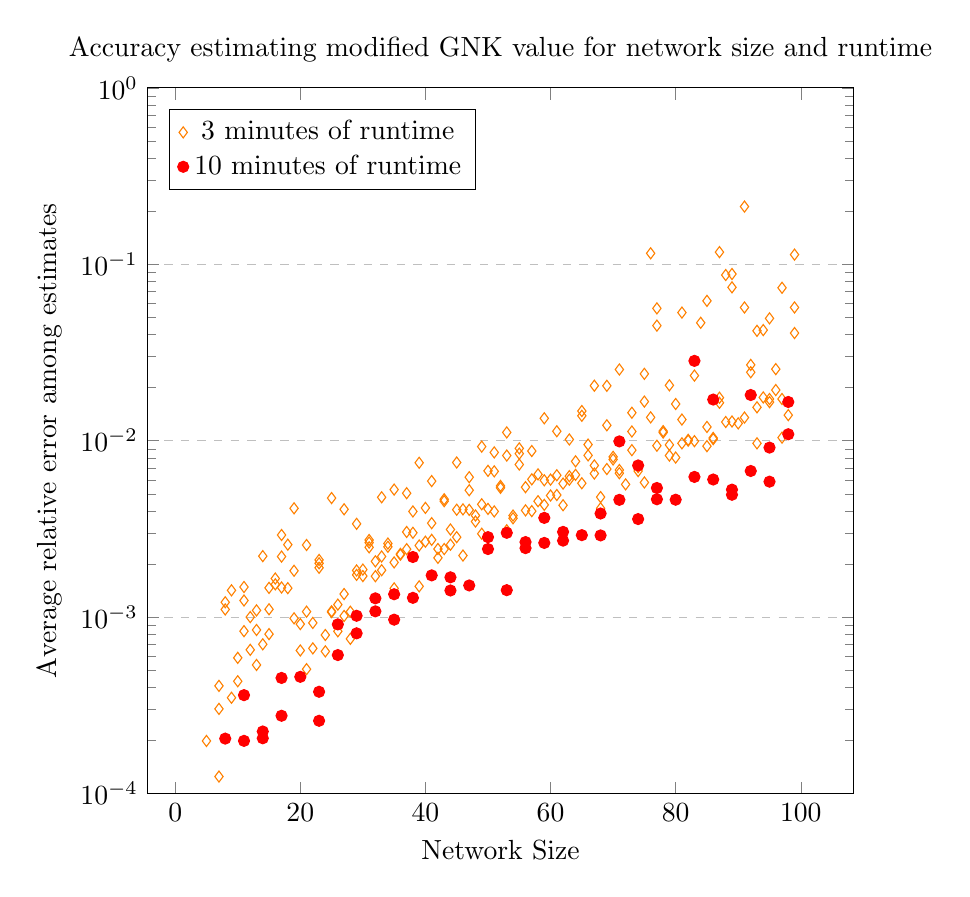
\begin{tikzpicture}
		\begin{axis}[
			title={Accuracy estimating modified GNK value for network size and runtime},
			xlabel={Network Size},
			ylabel={Average relative error among estimates},
			%xmin=0, xmax=0.25,
			ymin=0.0001, ymax=1.0,
			ymode=log,
			%xtick={0,0.05,0.1,0.15,0.2,0.25},
			%ytick={0,20,40,60,80,100},
			%yticklabel=$\pgfmathprintnumber{\tick}\%$,
			legend pos=north west,
			ymajorgrids=true,
			grid style=dashed,
			xticklabel style={/pgf/number format/fixed},
			width = 300,
			height = 300
		]
	%	\addplot [domain=5:15,dotted] {20+exp(exp(x/6.2))};
		\addplot[color=orange,only marks,mark=diamond] coordinates {
(7,0.000124846432046)
(9,0.000349362074085)
(11,0.00124222941518)
(13,0.00084580662349)
(15,0.000801583236527)
(17,0.00220431658342)
(19,0.00183164640034)
(21,0.0025649017953)
(23,0.00210995754038)
(25,0.00473061036627)
(27,0.00408531385556)
(29,0.00338104078055)
(31,0.00264677172477)
(33,0.0047801442004)
(35,0.00528516914309)
(37,0.00504239772522)
(39,0.00749977799528)
(41,0.00590305246372)
(43,0.00465727164346)
(45,0.00752693133478)
(47,0.00523965981561)
(49,0.00925944645823)
(51,0.00858391476366)
(53,0.0111435782515)
(55,0.00904646502096)
(57,0.00874408620603)
(59,0.0134009420369)
(61,0.0113124274953)
(63,0.0101657510766)
(65,0.0147341762157)
(67,0.0205141472091)
(69,0.0204764913685)
(71,0.0253312813336)
(73,0.0144118458985)
(75,0.02394286498)
(77,0.0449167019815)
(79,0.0206096637705)
(81,0.0532445997925)
(85,0.0620529404603)
(87,0.11719925893)
(89,0.074040615219)
(91,0.0569184449072)
(93,0.0419710612202)
(95,0.0493841921384)
(97,0.0736087900034)
(99,0.0569212660299)
(5,0.000198773008765)
(7,0.000407744729561)
(7,0.00030203334322)
(8,0.00121417461966)
(8,0.00110537817131)
(9,0.00141866481622)
(10,0.000587736031469)
(10,0.000433197835436)
(11,0.000833003424069)
(11,0.00148183780474)
(12,0.000652717485079)
(12,0.00100069147551)
(13,0.000535888589971)
(13,0.0010923780632)
(14,0.00221798060546)
(14,0.000701571822075)
(15,0.00146526302415)
(15,0.00110843825838)
(16,0.00153478099701)
(16,0.00165530968219)
(17,0.00147244059392)
(17,0.00292171158063)
(18,0.00257466150857)
(18,0.00146019035913)
(19,0.00413935310054)
(19,0.000984854650377)
(20,0.000913087823025)
(20,0.000647405471569)
(21,0.000506975456251)
(21,0.00107395672011)
(22,0.000927567910945)
(22,0.000665186002205)
(23,0.00201986852294)
(23,0.00190506406921)
(24,0.000639820142271)
(24,0.000792334026321)
(25,0.00107910701572)
(25,0.00106741530697)
(26,0.000831200889038)
(26,0.001178013224)
(27,0.00135186168514)
(27,0.00101545376012)
(28,0.00107335197392)
(28,0.000753723941028)
(29,0.00183920832934)
(29,0.00173603310834)
(30,0.00170985138939)
(30,0.00186055689586)
(31,0.00248752877425)
(31,0.00273821201003)
(32,0.00207141061644)
(32,0.00170630921974)
(33,0.00184563320948)
(33,0.00220666422401)
(34,0.00261345579349)
(34,0.00250566136421)
(35,0.00145532181738)
(35,0.00204272972711)
(36,0.00228404992204)
(36,0.00225933714185)
(37,0.00303894658767)
(37,0.0024283015975)
(38,0.00300795308548)
(38,0.00397239523048)
(39,0.0014948712232)
(39,0.00254757211551)
(40,0.00416220883856)
(40,0.00267674257379)
(41,0.00341086249742)
(41,0.00274167134022)
(42,0.00243460715137)
(42,0.00216802402016)
(43,0.0045429431476)
(43,0.00243201791179)
(44,0.00257436017038)
(44,0.0031394930501)
(45,0.00406347485638)
(45,0.00284040841552)
(46,0.00223361957965)
(46,0.00408187338654)
(47,0.00621155229259)
(47,0.00405687227955)
(48,0.00348237097269)
(48,0.0037691118267)
(49,0.00297039517578)
(49,0.00436222251494)
(50,0.006748950981)
(50,0.00410766447711)
(51,0.00670908443172)
(51,0.00397543990729)
(52,0.00554235567839)
(52,0.00540471876881)
(53,0.00824084761443)
(53,0.00310792483391)
(54,0.00363433436037)
(54,0.00376713945616)
(55,0.00844875182163)
(55,0.00732744960013)
(56,0.00402929471994)
(56,0.00545494825755)
(57,0.00399147611835)
(57,0.00604193725594)
(58,0.00454038668444)
(58,0.00644721921003)
(59,0.00596606446728)
(59,0.00432958920691)
(60,0.00601779650865)
(60,0.00489093054392)
(61,0.00492231997481)
(61,0.00637153496756)
(62,0.00430846933583)
(62,0.00571567178718)
(63,0.0060166079485)
(63,0.00629811025019)
(64,0.00640649255773)
(64,0.00763967913687)
(65,0.00573940477132)
(65,0.0138494680438)
(66,0.00950896711587)
(66,0.00826076933508)
(67,0.00651406615877)
(67,0.00724154201149)
(68,0.00479242033538)
(68,0.00414009158155)
(69,0.00691061325658)
(69,0.0122340696862)
(70,0.0081037292405)
(70,0.0078300002664)
(71,0.00654540779197)
(71,0.00682384509876)
(72,0.00565662022543)
(73,0.00884093704595)
(73,0.0112777832194)
(74,0.00708325114328)
(74,0.0067307025997)
(75,0.00580076774973)
(75,0.0166710544997)
(76,0.0135653233246)
(76,0.115409477308)
(77,0.0562417271889)
(77,0.00936786247095)
(78,0.0111215791274)
(78,0.0113334495573)
(79,0.00823906874579)
(79,0.00947459165119)
(80,0.0161486868496)
(80,0.00802704625735)
(81,0.00966195470957)
(81,0.0131841104013)
(82,0.0101128126268)
(82,0.0100115250202)
(83,0.00994581004764)
(83,0.0234048108537)
(84,0.0466033245366)
(85,0.00931630151593)
(85,0.0119695395793)
(86,0.0102139379601)
(86,0.0103722797318)
(87,0.0175397536068)
(87,0.0164074281767)
(88,0.0869332312724)
(88,0.0127678076343)
(89,0.0881032048071)
(89,0.0128528308022)
(90,0.0125394314882)
(91,0.21235279003)
(91,0.0135224949691)
(92,0.0269092164032)
(92,0.0244399626971)
(93,0.0154693117288)
(93,0.00966429818161)
(94,0.0423744311321)
(94,0.0176065608411)
(95,0.017242036729)
(95,0.0165513968124)
(96,0.0193783901172)
(96,0.0254570264808)
(97,0.0172404117218)
(97,0.0104124125146)
(98,0.0139618278174)
(99,0.0407574094971)
(99,0.113474875413)
			}node[pos=0.8](endofplotsquare){} ;
\addplot[color=red,only marks,mark=*] coordinates {
(8,0.000204879456534)
(11,0.000198954708294)
(14,0.000224818148859)
(17,0.000452273026779)
(23,0.000377511363366)
(26,0.000909889613207)
(29,0.000809735581049)
(32,0.00107871411898)
(35,0.00134833546078)
(38,0.00128650914677)
(44,0.00141620500018)
(50,0.00243255599249)
(53,0.00300619010686)
(56,0.00266403262447)
(59,0.00365306085279)
(62,0.00271466495323)
(68,0.00386736101309)
(71,0.00462278912607)
(74,0.0035967562431)
(77,0.00465761537595)
(80,0.00462987381052)
(83,0.00623532230411)
(86,0.0171156268226)
(89,0.00528077744006)
(92,0.00673753567814)
(95,0.00913995479916)
(98,0.0165834905391)
(5,0.0000773935779233)
(8,0.0000733345523358)
(11,0.000361375533438)
(14,0.000205841984163)
(17,0.000276048066766)
(20,0.000458867046201)
(23,0.000258513233782)
(26,0.000609668878525)
(29,0.00101805824417)
(32,0.0012780948209)
(35,0.000967653390575)
(38,0.00219240621832)
(41,0.00172504220769)
(44,0.00168192681336)
(47,0.00151247011605)
(50,0.00284133781795)
(53,0.00142210304518)
(56,0.00246181621126)
(59,0.00263488361456)
(62,0.00304277252977)
(65,0.00291604974117)
(68,0.00290600963346)
(71,0.00991308235081)
(74,0.00724174012946)
(77,0.00539653837363)
(83,0.0283508439613)
(86,0.00602785697971)
(89,0.00494013614493)
(92,0.0181610789112)
(95,0.00586061614028)
(98,0.010881684427)
			}node[pos=0.8](endofplotsquare){} ;
			
\addlegendentry{3 minutes of runtime}
\addlegendentry{10 minutes of runtime}
		\end{axis}
		\end{tikzpicture}
		%\vspace{-18pt}
		\caption{Average magnitude of error relative to the magnitude of the estimated modified GNK value between 8 independent simultaneous estimations on randomly generated networks of different sizes, for 3 and 10 minutes runtime on a desktop computer.}
		\label{fig:performance_graph4}
    \end{figure}




\end{frame}
\begin{frame}



\begin{figure}[h!]
    \centering
    \begin{minipage}{0.48\textwidth}
        \centering

\begin{tikzpicture}
\begin{axis}[width=7cm, height=8cm, view={30}{30},
%colormap/viridis,
point meta min=-1.0, point meta max=9.0,
%colorbar,
xlabel=x,
ylabel=y,
%zlabel=z,
grid=major]
\addplot3[only marks, scatter]
table[x index=0, y index=1, z index=2, point meta=z, col sep=comma]{data/lmp_out_csv.csv};
\end{axis}
\end{tikzpicture}

\caption[Utility payments under LMP for 90 bus network]{Post payment utility under LMP against consumption/geneation capacity (x) with per-unit utility (y)}
\label{fig:experiment_table_11}
    \end{minipage}\hfill
    \begin{minipage}{0.48\textwidth}
        \centering

\begin{tikzpicture}
\begin{axis}[width=7cm, height=8cm, view={30}{30},
%colormap/viridis,
point meta min=-1.0, point meta max=9.0,
colorbar,
xlabel=x,
ylabel=y,
%zlabel=z,
grid=major]
\addplot3[only marks, scatter]
table[x index=0, y index=1, z index=2, point meta=z, col sep=comma]{data/vcg_out_csv.csv};
\end{axis}
\end{tikzpicture}

\caption[Utility payments under VCG for 90 bus network]{Post payment utility under VCG against consumption/geneation capacity (x) with per-unit utility (y)}
\label{fig:experiment_table_12}
    \end{minipage}\vspace{10mm}
    \begin{minipage}{0.48\textwidth}
        \centering

\begin{tikzpicture}
\begin{axis}[width=7cm, height=8cm, view={30}{30},
%colormap/viridis,
point meta min=-1.0, point meta max=9.0,
%colorbar,
xlabel=x,
ylabel=y,
%zlabel=z,
grid=major]
\addplot3[only marks, scatter]
table[x index=0, y index=1, z index=2, point meta=z, col sep=comma]{data/gnk_out_csv.csv};
\end{axis}
\end{tikzpicture}

\caption[Utility payments under modified-GNK for 90 bus network]{Post payment utility under proxy GNK against consumption/geneation capacity (x) with per-unit utility (y)}
\label{fig:experiment_table_13}
    \end{minipage}\hfill
    \begin{minipage}{0.48\textwidth}
        \centering

\resizebox*{1.0\columnwidth} {!} {
    \begin {tikzpicture}

\draw[line width=0.8pt] (0.44096136990388646,-0.5618691934735468) -- (1.069800579089067,0.16548093436720387);
\draw[line width=0.8pt] (1.069800579089067,0.16548093436720387) -- (1.4853312258077276,-0.8500116223199463);
\draw[line width=0.8pt] (0.44096136990388646,-0.5618691934735468) -- (1.4853312258077276,-0.8500116223199463);
\draw[line width=0.8pt] (1.4853312258077276,-0.8500116223199463) -- (2.1489085420475624,-1.0713594955405452);
\draw[line width=0.8pt] (0.44096136990388646,-0.5618691934735468) -- (0.1811494487782036,-1.833998077644877);
\draw[line width=0.8pt] (0.1811494487782036,-1.833998077644877) -- (-0.8131937383015331,-2.535177527702246);
\draw[line width=0.8pt] (1.4853312258077276,-0.8500116223199463) -- (1.9736544604359036,-0.34339646113732064);
\draw[line width=0.8pt] (-0.8131937383015331,-2.535177527702246) -- (-0.7876012028017446,-3.076409487117164);
\draw[line width=0.8pt] (0.44096136990388646,-0.5618691934735468) -- (-0.7954021216306426,-0.5455459684144736);
\draw[line width=0.8pt] (-0.7876012028017446,-3.076409487117164) -- (-0.5984380344340882,-3.8287539330858302);
\draw[line width=0.8pt] (2.1489085420475624,-1.0713594955405452) -- (2.6904208271332575,-1.285723259906219);
\draw[line width=0.8pt] (0.44096136990388646,-0.5618691934735468) -- (0.07932091229496825,0.7318680994982809);
\draw[line width=0.8pt] (1.069800579089067,0.16548093436720387) -- (0.07932091229496825,0.7318680994982809);
\draw[line width=0.8pt] (-0.8131937383015331,-2.535177527702246) -- (-1.8072605158231962,-2.449349890827679);
\draw[line width=0.8pt] (0.07932091229496825,0.7318680994982809) -- (-0.5978155164396761,0.9614870055786316);
\draw[line width=0.8pt] (0.44096136990388646,-0.5618691934735468) -- (-0.5978155164396761,0.9614870055786316);
\draw[line width=0.8pt] (-1.8072605158231962,-2.449349890827679) -- (-1.875596139204054,-1.6096770607938309);
\draw[line width=0.8pt] (-0.5978155164396761,0.9614870055786316) -- (-0.5970344286855532,1.770655959571318);
\draw[line width=0.8pt] (-0.5970344286855532,1.770655959571318) -- (-1.4697249713947735,1.803799891240862);
\draw[line width=0.8pt] (-0.5978155164396761,0.9614870055786316) -- (-1.4697249713947735,1.803799891240862);
\draw[line width=0.8pt] (2.6904208271332575,-1.285723259906219) -- (3.7750304643446193,-0.34057570937918324);
\draw[line width=0.8pt] (0.44096136990388646,-0.5618691934735468) -- (0.6024557429218482,-1.781310322204095);
\draw[line width=0.8pt] (0.1811494487782036,-1.833998077644877) -- (0.6024557429218482,-1.781310322204095);
\draw[line width=0.8pt] (1.069800579089067,0.16548093436720387) -- (1.8053447214341394,1.1017032436206948);
\draw[line width=0.8pt] (-0.7954021216306426,-0.5455459684144736) -- (-1.125627506859321,0.05006845877500168);
\draw[line width=0.8pt] (-0.7954021216306426,-0.5455459684144736) -- (-1.0942259106033339,-1.0086145041945658);
\draw[line width=0.8pt] (1.8053447214341394,1.1017032436206948) -- (2.4559125867899585,1.6389576402178223);
\draw[line width=0.8pt] (3.7750304643446193,-0.34057570937918324) -- (3.052069093653992,-0.21332976797089676);
\draw[line width=0.8pt] (2.6904208271332575,-1.285723259906219) -- (3.052069093653992,-0.21332976797089676);
\draw[line width=0.8pt] (-0.5978155164396761,0.9614870055786316) -- (-1.3283495112291275,1.2115065363880673);
\draw[line width=0.8pt] (-1.4697249713947735,1.803799891240862) -- (-1.3283495112291275,1.2115065363880673);
\draw[line width=0.8pt] (0.44096136990388646,-0.5618691934735468) -- (1.3317987391902217,-2.025965931741168);
\draw[line width=0.8pt] (0.6024557429218482,-1.781310322204095) -- (1.3317987391902217,-2.025965931741168);
\draw[line width=0.8pt] (2.4559125867899585,1.6389576402178223) -- (1.6885533505391104,1.9760239036809943);
\draw[line width=0.8pt] (-1.8072605158231962,-2.449349890827679) -- (-2.581342454614481,-2.278320026488054);
\draw[line width=0.8pt] (-1.875596139204054,-1.6096770607938309) -- (-2.581342454614481,-2.278320026488054);
\draw[line width=0.8pt] (-1.0942259106033339,-1.0086145041945658) -- (-0.551459688315166,-1.5783292498763546);
\draw[line width=0.8pt] (-0.7954021216306426,-0.5455459684144736) -- (-0.551459688315166,-1.5783292498763546);
\draw[line width=0.8pt] (2.4559125867899585,1.6389576402178223) -- (2.8824667060051157,1.4267264740479781);
\draw[line width=0.8pt] (-1.4697249713947735,1.803799891240862) -- (-2.61690901096465,1.7762186383799616);
\draw[line width=0.8pt] (-1.3283495112291275,1.2115065363880673) -- (-1.900013750014958,1.171942945390202);
\draw[line width=0.8pt] (1.8053447214341394,1.1017032436206948) -- (1.1873145452004636,1.5631852814681244);
\draw[line width=0.8pt] (1.6885533505391104,1.9760239036809943) -- (1.1873145452004636,1.5631852814681244);
\draw[line width=0.8pt] (-1.125627506859321,0.05006845877500168) -- (-1.489849824408247,0.4395410311956199);
\draw[line width=0.8pt] (1.3317987391902217,-2.025965931741168) -- (2.0766747523267894,-3.0051231025709013);
\draw[line width=0.8pt] (-0.5984380344340882,-3.8287539330858302) -- (-0.12217712951845208,-3.386960947940069);
\draw[line width=0.8pt] (-0.7876012028017446,-3.076409487117164) -- (-0.12217712951845208,-3.386960947940069);
\draw[line width=0.8pt] (-2.61690901096465,1.7762186383799616) -- (-3.420834380792476,1.1639087313755327);
\draw[line width=0.8pt] (1.069800579089067,0.16548093436720387) -- (1.584562739411188,0.1309805472956378);
\draw[line width=0.8pt] (1.9736544604359036,-0.34339646113732064) -- (1.584562739411188,0.1309805472956378);
\draw[line width=0.8pt] (2.0766747523267894,-3.0051231025709013) -- (2.505144251601519,-3.6403747681290985);
\draw[line width=0.8pt] (0.07932091229496825,0.7318680994982809) -- (0.10624560578140362,1.2755024890589723);
\draw[line width=0.8pt] (-1.900013750014958,1.171942945390202) -- (-2.461944204549911,0.8481319105032009);
\draw[line width=0.8pt] (-0.7954021216306426,-0.5455459684144736) -- (-1.528891632413253,-0.5785470905769897);
\draw[line width=0.8pt] (1.3317987391902217,-2.025965931741168) -- (2.0526518892834726,-2.149068191906359);
\draw[line width=0.8pt] (-0.7954021216306426,-0.5455459684144736) -- (-0.4413034696565202,-0.1460340258918184);
\draw[line width=0.8pt] (0.6024557429218482,-1.781310322204095) -- (0.5673782622776348,-2.763810388190237);
\draw[line width=0.8pt] (0.1811494487782036,-1.833998077644877) -- (0.5673782622776348,-2.763810388190237);
\draw[line width=0.8pt] (-0.551459688315166,-1.5783292498763546) -- (-0.8724175878699774,-2.180155779960795);
\draw[line width=0.8pt] (0.6024557429218482,-1.781310322204095) -- (0.9336662988281781,-2.549975444008825);
\draw[line width=0.8pt] (1.8053447214341394,1.1017032436206948) -- (1.923828420503969,0.4313728053400574);
\draw[line width=0.8pt] (1.8053447214341394,1.1017032436206948) -- (2.6442442895533538,0.6292437823753158);
\draw[line width=0.8pt] (2.4559125867899585,1.6389576402178223) -- (3.173117532266346,1.8385686777325643);
\draw[line width=0.8pt] (-2.461944204549911,0.8481319105032009) -- (-2.7369747613640536,0.309921620763573);
\draw[line width=0.8pt] (1.3317987391902217,-2.025965931741168) -- (1.44196588267486,-2.867644153840621);
\draw[line width=0.8pt] (-2.581342454614481,-2.278320026488054) -- (-3.2501990459004846,-1.9076012765040558);
\draw[line width=0.8pt] (2.6904208271332575,-1.285723259906219) -- (1.9561659029754037,-1.683701402461596);
\draw[line width=0.8pt] (1.6885533505391104,1.9760239036809943) -- (2.3436602273242246,2.3208800498944133);
\draw[line width=0.8pt] (2.4559125867899585,1.6389576402178223) -- (2.3436602273242246,2.3208800498944133);
\draw[line width=0.8pt] (0.5673782622776348,-2.763810388190237) -- (0.8878722052903494,-3.5388004610923);
\draw[line width=0.8pt] (-2.7369747613640536,0.309921620763573) -- (-2.1517057630574676,0.19158989845756674);
\draw[line width=0.8pt] (-0.5970344286855532,1.770655959571318) -- (-0.4304026240261578,2.43084807937398);
\draw[line width=0.8pt] (-1.875596139204054,-1.6096770607938309) -- (-2.5597660227701935,-1.0910209596649094);
\draw[line width=0.8pt] (-2.581342454614481,-2.278320026488054) -- (-2.5597660227701935,-1.0910209596649094);
\draw[line width=0.8pt] (-0.8724175878699774,-2.180155779960795) -- (-1.1950952422141148,-1.7014334251864698);
\draw[line width=0.8pt] (0.07932091229496825,0.7318680994982809) -- (0.4891364415039052,1.6302134577610852);
\draw[line width=0.8pt] (0.10624560578140362,1.2755024890589723) -- (0.4891364415039052,1.6302134577610852);
\draw[line width=0.8pt] (0.07932091229496825,0.7318680994982809) -- (0.5643607123708261,1.0358380970674244);
\draw[line width=0.8pt] (0.4891364415039052,1.6302134577610852) -- (0.5643607123708261,1.0358380970674244);
\draw[line width=0.8pt] (1.9561659029754037,-1.683701402461596) -- (2.7771853457071525,-2.006046278845794);
\draw[line width=0.8pt] (2.6904208271332575,-1.285723259906219) -- (2.7771853457071525,-2.006046278845794);
\draw[line width=0.8pt] (-0.4304026240261578,2.43084807937398) -- (0.03101884354467703,2.4553260066795475);
\draw[line width=0.8pt] (-3.420834380792476,1.1639087313755327) -- (-3.8057373754008736,0.18505967021297118);
\draw[line width=0.8pt] (0.5673782622776348,-2.763810388190237) -- (0.1329144509474538,-2.3847488854863803);
\draw[line width=0.8pt] (0.1811494487782036,-1.833998077644877) -- (0.1329144509474538,-2.3847488854863803);
\draw[line width=0.8pt] (1.4853312258077276,-0.8500116223199463) -- (2.48691136616922,-0.23442719599915962);
\draw[line width=0.8pt] (2.6442442895533538,0.6292437823753158) -- (2.48691136616922,-0.23442719599915962);
\draw[line width=0.8pt] (-1.528891632413253,-0.5785470905769897) -- (-2.0481225313766562,-0.6726851408822385);
\draw[line width=0.8pt] (-3.8057373754008736,0.18505967021297118) -- (-3.7416258991978895,-0.9051535182695852);
\draw[line width=0.8pt] (-3.2501990459004846,-1.9076012765040558) -- (-3.7416258991978895,-0.9051535182695852);
\draw[line width=0.8pt] (-1.4697249713947735,1.803799891240862) -- (-1.850157178722093,2.5724966087219947);
\draw[line width=0.8pt] (0.03101884354467703,2.4553260066795475) -- (0.025656380533700975,1.823814404074668);
\draw[line width=0.8pt] (-0.5970344286855532,1.770655959571318) -- (0.025656380533700975,1.823814404074668);
\draw[line width=0.8pt] (-0.5970344286855532,1.770655959571318) -- (-1.0881007806138798,2.4377316023113056);
\draw[line width=0.8pt] (0.5673782622776348,-2.763810388190237) -- (0.45947808126408074,-3.804536840780034);
\draw[line width=0.8pt] (-0.12217712951845208,-3.386960947940069) -- (-0.09620266816923893,-2.7987849875495585);
\draw[line width=0.8pt] (-0.7876012028017446,-3.076409487117164) -- (-0.09620266816923893,-2.7987849875495585);
\draw[line width=0.8pt] (3.7750304643446193,-0.34057570937918324) -- (3.5822888698417987,0.17705848593906873);
\draw[line width=0.8pt] (3.052069093653992,-0.21332976797089676) -- (3.5822888698417987,0.17705848593906873);
\draw[line width=0.8pt] (3.7750304643446193,-0.34057570937918324) -- (4.313127612974511,-0.8110027784226188);
\draw[line width=0.8pt] (3.5822888698417987,0.17705848593906873) -- (3.4535151666012602,0.7733849660828275);
\draw[line width=0.8pt] (0.4891364415039052,1.6302134577610852) -- (0.6758209406688575,2.560599693016568);
\draw[line width=0.8pt] (1.44196588267486,-2.867644153840621) -- (1.64322868634623,-3.73027760221179);
\draw[line width=0.8pt] (2.6904208271332575,-1.285723259906219) -- (3.3236785193438774,-1.2729422550217295);
\draw[line width=0.8pt] (-1.8072605158231962,-2.449349890827679) -- (-2.187483446216561,-3.1353040842401447);
\draw[line width=0.8pt] (-0.5984380344340882,-3.8287539330858302) -- (-1.3006825007406135,-3.602241383459367);
\draw[line width=0.8pt] (1.6885533505391104,1.9760239036809943) -- (1.5729959420327198,2.564767994125724);
\draw[line width=0.8pt] (3.173117532266346,1.8385686777325643) -- (3.3285505135636146,2.6563594548571623);
\draw[line width=0.8pt] (2.7771853457071525,-2.006046278845794) -- (3.3044213861347354,-2.512653971629536);
\draw[line width=0.8pt] (-3.2501990459004846,-1.9076012765040558) -- (-3.3319212434764554,-2.644218019747517);
\draw[line width=0.8pt] (3.7750304643446193,-0.34057570937918324) -- (4.422563130958106,-0.06665697535949511);
\draw[line width=0.8pt] (-2.7369747613640536,0.309921620763573) -- (-2.8157235152533495,-0.33593836929963217);
\draw[line width=0.8pt] (-2.5597660227701935,-1.0910209596649094) -- (-2.8157235152533495,-0.33593836929963217);
\draw[line width=0.8pt] (0.1811494487782036,-1.833998077644877) -- (0.03598144943524574,-1.0217786644985);
\draw[line width=0.8pt] (3.173117532266346,1.8385686777325643) -- (3.791637430996665,2.145254152563245);













\draw[black,fill=white] (0.44096136990388646,-0.5618691934735468) circle (0.08);
\draw[black,fill=white] (1.069800579089067,0.16548093436720387) circle (0.08);
\draw[black,fill=white] (1.4853312258077276,-0.8500116223199463) circle (0.08);
\draw[black,fill=white] (2.1489085420475624,-1.0713594955405452) circle (0.08);
\draw[black,fill=white] (0.1811494487782036,-1.833998077644877) circle (0.08);
\draw[black,fill=white] (-0.8131937383015331,-2.535177527702246) circle (0.08);
\draw[black,fill=white] (1.9736544604359036,-0.34339646113732064) circle (0.08);
\draw[black,fill=white] (-0.7876012028017446,-3.076409487117164) circle (0.08);
\draw[black,fill=white] (-0.7954021216306426,-0.5455459684144736) circle (0.08);
\draw[black,fill=white] (-0.5984380344340882,-3.8287539330858302) circle (0.08);
\draw[black,fill=white] (2.6904208271332575,-1.285723259906219) circle (0.08);
\draw[black,fill=white] (0.07932091229496825,0.7318680994982809) circle (0.08);
\draw[black,fill=white] (-1.8072605158231962,-2.449349890827679) circle (0.08);
\draw[black,fill=white] (-0.5978155164396761,0.9614870055786316) circle (0.08);
\draw[black,fill=white] (-1.875596139204054,-1.6096770607938309) circle (0.08);
\draw[black,fill=white] (-0.5970344286855532,1.770655959571318) circle (0.08);
\draw[black,fill=white] (-1.4697249713947735,1.803799891240862) circle (0.08);
\draw[black,fill=white] (3.7750304643446193,-0.34057570937918324) circle (0.08);
\draw[black,fill=white] (0.6024557429218482,-1.781310322204095) circle (0.08);
\draw[black,fill=white] (1.8053447214341394,1.1017032436206948) circle (0.08);
\draw[black,fill=white] (-1.125627506859321,0.05006845877500168) circle (0.08);
\draw[black,fill=white] (-1.0942259106033339,-1.0086145041945658) circle (0.08);
\draw[black,fill=white] (2.4559125867899585,1.6389576402178223) circle (0.08);
\draw[black,fill=white] (3.052069093653992,-0.21332976797089676) circle (0.08);
\draw[black,fill=white] (-1.3283495112291275,1.2115065363880673) circle (0.08);
\draw[black,fill=white] (1.3317987391902217,-2.025965931741168) circle (0.08);
\draw[black,fill=white] (1.6885533505391104,1.9760239036809943) circle (0.08);
\draw[black,fill=white] (-2.581342454614481,-2.278320026488054) circle (0.08);
\draw[black,fill=white] (-0.551459688315166,-1.5783292498763546) circle (0.08);
\draw[black,fill=white] (2.8824667060051157,1.4267264740479781) circle (0.08);
\draw[black,fill=white] (-2.61690901096465,1.7762186383799616) circle (0.08);
\draw[black,fill=white] (-1.900013750014958,1.171942945390202) circle (0.08);
\draw[black,fill=white] (1.1873145452004636,1.5631852814681244) circle (0.08);
\draw[black,fill=white] (-1.489849824408247,0.4395410311956199) circle (0.08);
\draw[black,fill=white] (2.0766747523267894,-3.0051231025709013) circle (0.08);
\draw[black,fill=white] (-0.12217712951845208,-3.386960947940069) circle (0.08);
\draw[black,fill=white] (-3.420834380792476,1.1639087313755327) circle (0.08);
\draw[black,fill=white] (1.584562739411188,0.1309805472956378) circle (0.08);
\draw[black,fill=white] (2.505144251601519,-3.6403747681290985) circle (0.08);
\draw[black,fill=white] (0.10624560578140362,1.2755024890589723) circle (0.08);
\draw[black,fill=white] (-2.461944204549911,0.8481319105032009) circle (0.08);
\draw[black,fill=white] (-1.528891632413253,-0.5785470905769897) circle (0.08);
\draw[black,fill=white] (2.0526518892834726,-2.149068191906359) circle (0.08);
\draw[black,fill=white] (-0.4413034696565202,-0.1460340258918184) circle (0.08);
\draw[black,fill=white] (0.5673782622776348,-2.763810388190237) circle (0.08);
\draw[black,fill=white] (-0.8724175878699774,-2.180155779960795) circle (0.08);

\draw[black,fill=black] (0.9336662988281781,-2.549975444008825) circle (0.08);
\draw[black,fill=black] (1.923828420503969,0.4313728053400574) circle (0.08);
\draw[black,fill=black] (2.6442442895533538,0.6292437823753158) circle (0.08);
\draw[black,fill=black] (3.173117532266346,1.8385686777325643) circle (0.08);
\draw[black,fill=black] (-2.7369747613640536,0.309921620763573) circle (0.08);
\draw[black,fill=black] (1.44196588267486,-2.867644153840621) circle (0.08);
\draw[black,fill=black] (-3.2501990459004846,-1.9076012765040558) circle (0.08);
\draw[black,fill=black] (1.9561659029754037,-1.683701402461596) circle (0.08);
\draw[black,fill=black] (2.3436602273242246,2.3208800498944133) circle (0.08);
\draw[black,fill=black] (0.8878722052903494,-3.5388004610923) circle (0.08);
\draw[black,fill=black] (-2.1517057630574676,0.19158989845756674) circle (0.08);
\draw[black,fill=black] (-0.4304026240261578,2.43084807937398) circle (0.08);
\draw[black,fill=black] (-2.5597660227701935,-1.0910209596649094) circle (0.08);
\draw[black,fill=black] (-1.1950952422141148,-1.7014334251864698) circle (0.08);
\draw[black,fill=black] (0.4891364415039052,1.6302134577610852) circle (0.08);
\draw[black,fill=black] (0.5643607123708261,1.0358380970674244) circle (0.08);
\draw[black,fill=black] (2.7771853457071525,-2.006046278845794) circle (0.08);
\draw[black,fill=black] (0.03101884354467703,2.4553260066795475) circle (0.08);
\draw[black,fill=black] (-3.8057373754008736,0.18505967021297118) circle (0.08);
\draw[black,fill=black] (0.1329144509474538,-2.3847488854863803) circle (0.08);
\draw[black,fill=black] (2.48691136616922,-0.23442719599915962) circle (0.08);
\draw[black,fill=black] (-2.0481225313766562,-0.6726851408822385) circle (0.08);
\draw[black,fill=black] (-3.7416258991978895,-0.9051535182695852) circle (0.08);
\draw[black,fill=black] (-1.850157178722093,2.5724966087219947) circle (0.08);
\draw[black,fill=black] (0.025656380533700975,1.823814404074668) circle (0.08);
\draw[black,fill=black] (-1.0881007806138798,2.4377316023113056) circle (0.08);
\draw[black,fill=black] (0.45947808126408074,-3.804536840780034) circle (0.08);
\draw[black,fill=black] (-0.09620266816923893,-2.7987849875495585) circle (0.08);
\draw[black,fill=black] (3.5822888698417987,0.17705848593906873) circle (0.08);
\draw[black,fill=black] (4.313127612974511,-0.8110027784226188) circle (0.08);
\draw[black,fill=black] (3.4535151666012602,0.7733849660828275) circle (0.08);
\draw[black,fill=black] (0.6758209406688575,2.560599693016568) circle (0.08);
\draw[black,fill=black] (1.64322868634623,-3.73027760221179) circle (0.08);
\draw[black,fill=black] (3.3236785193438774,-1.2729422550217295) circle (0.08);
\draw[black,fill=black] (-2.187483446216561,-3.1353040842401447) circle (0.08);
\draw[black,fill=black] (-1.3006825007406135,-3.602241383459367) circle (0.08);
\draw[black,fill=black] (1.5729959420327198,2.564767994125724) circle (0.08);
\draw[black,fill=black] (3.3285505135636146,2.6563594548571623) circle (0.08);
\draw[black,fill=black] (3.3044213861347354,-2.512653971629536) circle (0.08);
\draw[black,fill=black] (-3.3319212434764554,-2.644218019747517) circle (0.08);
\draw[black,fill=black] (4.422563130958106,-0.06665697535949511) circle (0.08);
\draw[black,fill=black] (-2.8157235152533495,-0.33593836929963217) circle (0.08);
\draw[black,fill=black] (0.03598144943524574,-1.0217786644985) circle (0.08);
\draw[black,fill=black] (3.791637430996665,2.145254152563245) circle (0.08);


    \end {tikzpicture}
}
\caption[Node-line diagram for 90 bus network]{Node-line diagram for the example randomly generated 90-bus system, showing a 50-50 mix of small generators (black) and consumers (white)}
\label{fig:experiment_table_14}

    \end{minipage}
\end{figure}











\end{frame}


%----------------------------------------------------------------------------------------
%	PRESENTATION SLIDES
%----------------------------------------------------------------------------------------

\begin{frame}
\frametitle{Theorem}
\begin{theorem}[Mass--energy equivalence]
$E = mc^2$
\end{theorem}
\end{frame}

%------------------------------------------------

\begin{frame}[fragile] % Need to use the fragile option when verbatim is used in the slide
\frametitle{Verbatim}
\begin{example}[Theorem Slide Code]
\begin{verbatim}
\begin{frame}
\frametitle{Theorem}
\begin{theorem}[Mass--energy equivalence]
$E = mc^2$
\end{theorem}
\end{frame}\end{verbatim}
\end{example}
\end{frame}

%------------------------------------------------

\begin{frame}
\frametitle{Figure}
Uncomment the code on this slide to include your own image from the same directory as the template .TeX file.
%\begin{figure}
%\includegraphics[width=0.8\linewidth]{test}
%\end{figure}
\end{frame}

%------------------------------------------------

\begin{frame}[fragile] % Need to use the fragile option when verbatim is used in the slide
\frametitle{Citation}
An example of the \verb|\cite| command to cite within the presentation:\\~

This statement requires citation \cite{p1}.
\end{frame}

%------------------------------------------------

\begin{frame}
\frametitle{References}
\footnotesize{
\begin{thebibliography}{99} % Beamer does not support BibTeX so references must be inserted manually as below
\bibitem[Smith, 2012]{p1} John Smith (2012)
\newblock Title of the publication
\newblock \emph{Journal Name} 12(3), 45 -- 678.
\end{thebibliography}
}
\end{frame}

%------------------------------------------------

\begin{frame}
\Huge{\centerline{The End}}
\end{frame}

%----------------------------------------------------------------------------------------

\end{document} 
